\chapter{Appendix}

\section{Code Examples}

\subsection{Matlab code for the Hybrid Network Classifier}
\lstinputlisting[language=Matlab,firstline=559, lastline=605, caption= Matlab code for the Hybrid Network Classifier, label={lst:Matlab code for the Hybrid Network Classifier}]{Code/networksAll.m}

\subsection{Automating 12 runs of 12 sets of validation images}
\lstinputlisting[language=Matlab, caption= Matlab code for automating 12 runs of 12 sets of validation images, label={lst:Automating 12 runs of 12 sets of validation images}]{Code/automatedTwelveRuns.m}

\subsection{Analysis and Visualisation of Feature Ratings Correlation}
\begin{figure}[H]
  \centering
    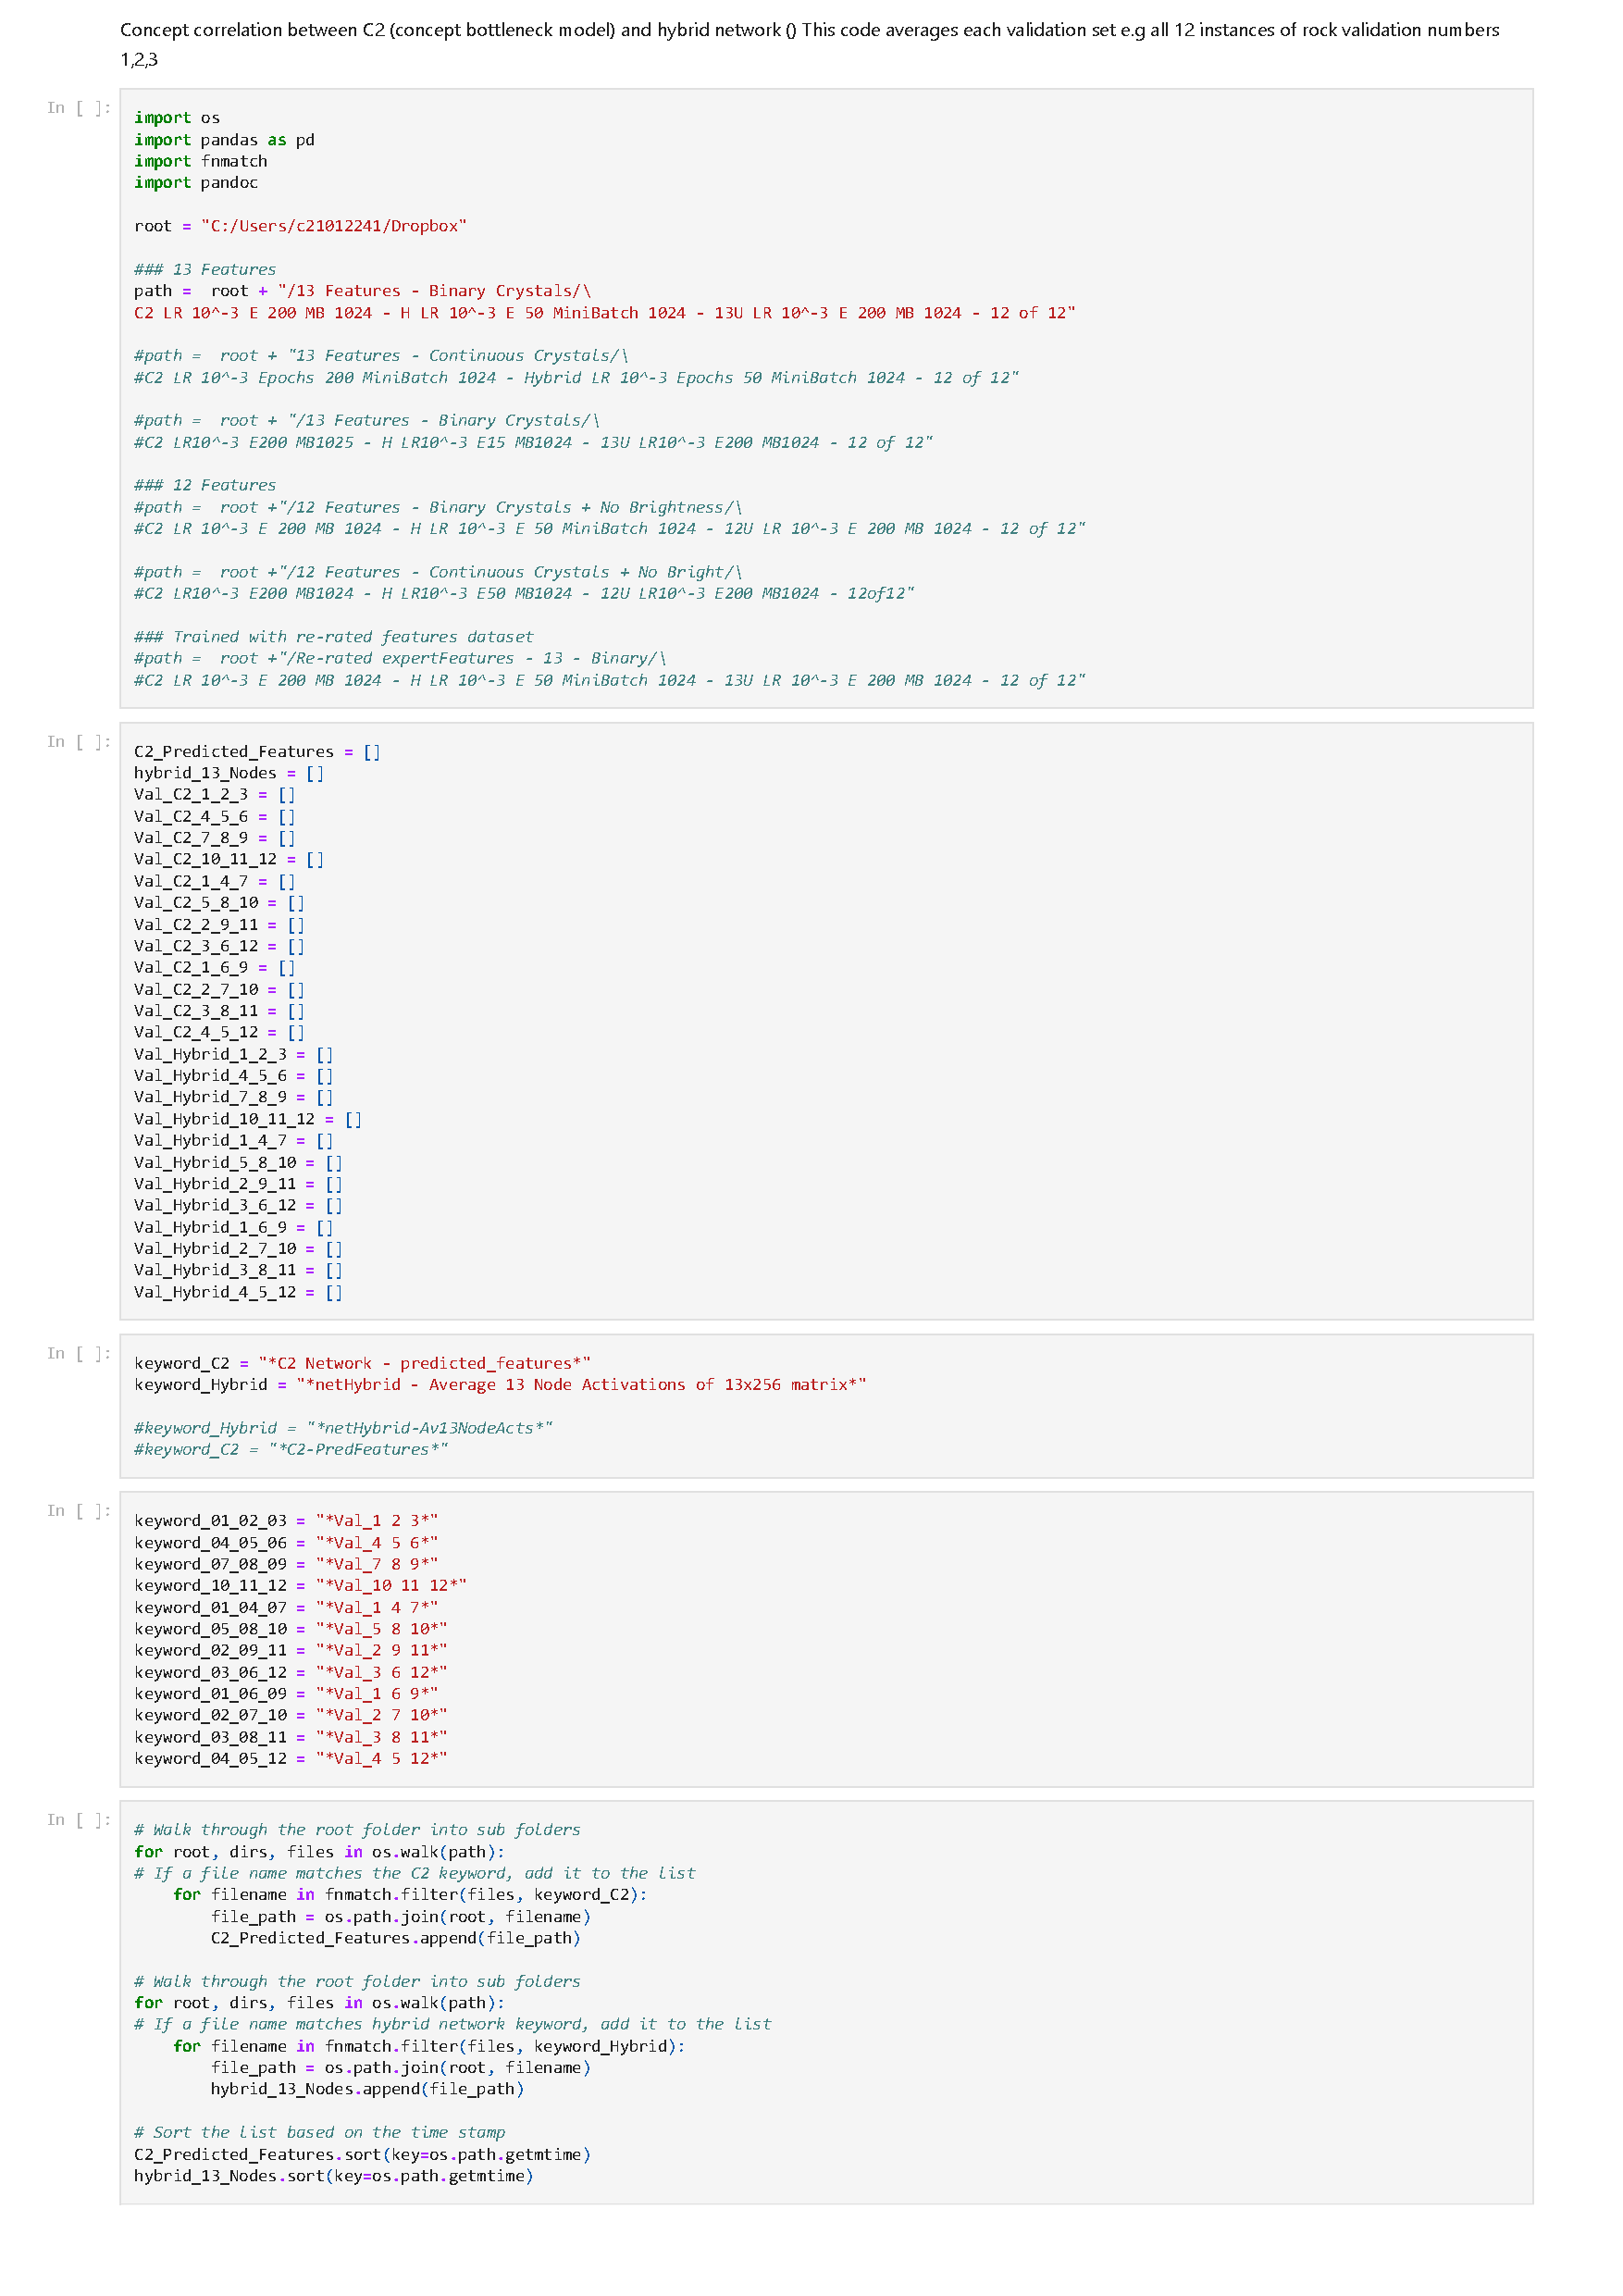
\includegraphics[width=0.92\textwidth, height=0.92\textheight]{Code/Correlation_Visualisation_and_CSV_for_Average_Feature_Ratings_-_12_of_12.pdf}
  \label{fig:Correlation Visualisation for Average Feature Ratings}
\end{figure}
\includepdf[pages=2-6, width=0.92\textwidth, height=0.92\textheight]{Code/Correlation_Visualisation_and_CSV_for_Average_Feature_Ratings_-_12_of_12.pdf}
\begin{figure}[H]
  \centering
    \includegraphics[page=7, width=0.92\textwidth, trim= 20 500 20 0, clip]{Code/Correlation_Visualisation_and_CSV_for_Average_Feature_Ratings_-_12_of_12.pdf}
    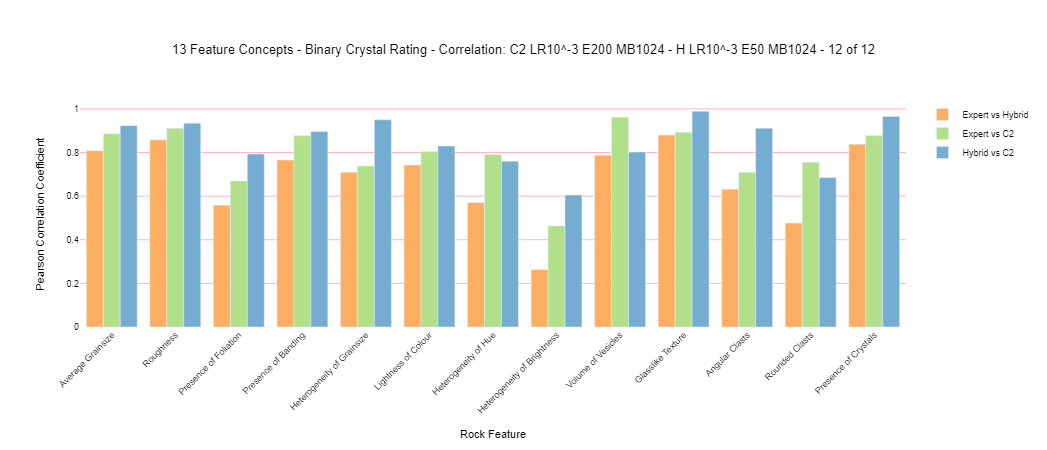
\includegraphics[width=0.92\textwidth, trim = 1cm 0.2cm 0.5cm 0, clip]{images/13 Feature Concepts - Binary Crystal Rating - Correlation- C2 LR10^-3 E200 MB1024 - H LR10^-3 E50 MB1024 - 12 of 12.png}
    \caption{Code for the Analysis and Visualisation of Pearson's Correlation Co-Efficient of Feature Ratings Between Expert Feature Ratings, Sequential CBM and Hybrid Classifier CBM. This was coded using Python in a Jupyter Notebook, and Plotly for visualisation} \label{fig:Code for the Analysis and Visualisation of Pearson's Correlation Co-Efficient of Feature Ratings Between Expert Feature Ratings, Sequential CBM and Hybrid Classifier CBM}
\end{figure}

\subsection{Means and Standard Error of the Mean (SEM) - Analysis and Visualisation using Plotly}
\begin{figure}[H]
  \centering
    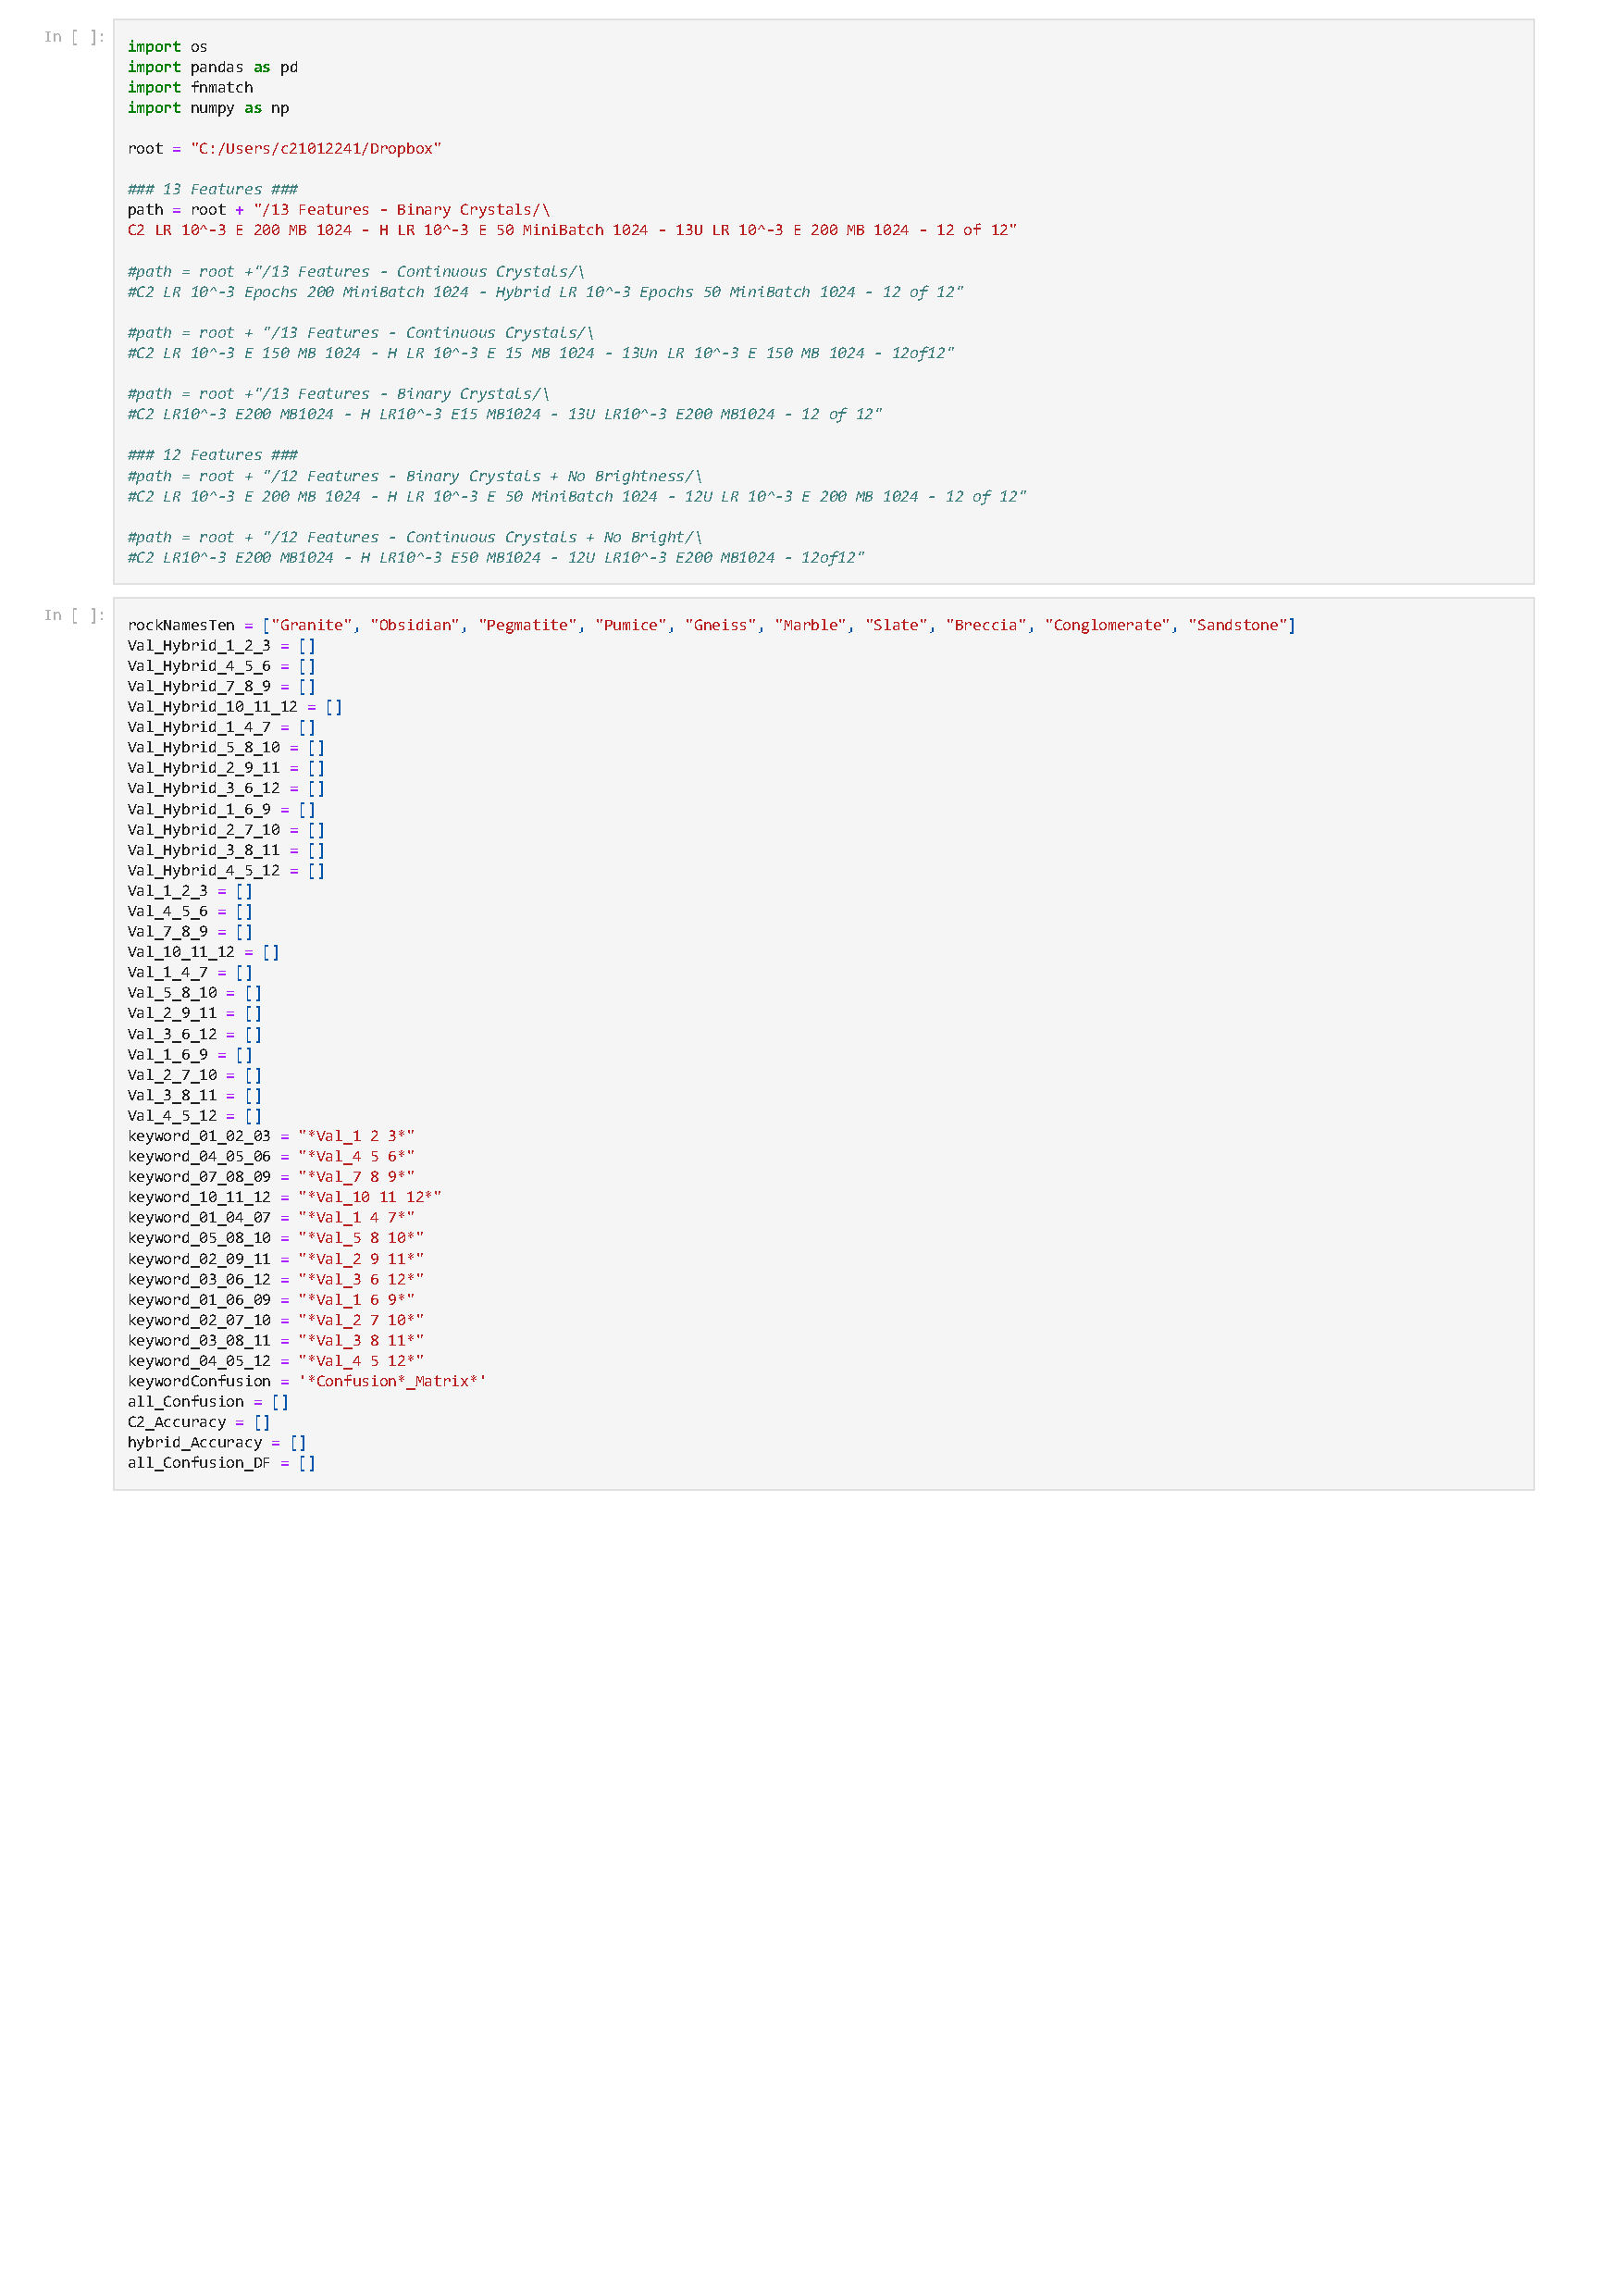
\includegraphics[width=0.99\textwidth, height=0.99\textheight]{Code/Mean_and_SEM_-_Visualisation_of_12_of_12_Validation_Sets.pdf}
  \label{fig:Mean_and_SEM_-_Visualisation_of_12_of_12_Validation_Sets}
\end{figure}
\includepdf[pages=2-6, width=0.99\textwidth, height=0.99\textheight]{Code/Mean_and_SEM_-_Visualisation_of_12_of_12_Validation_Sets.pdf}
\begin{figure}[H]
  \centering
    \includegraphics[page=7, width=0.95\textwidth, trim= 20 450 20 10, clip]{Code/Mean_and_SEM_-_Visualisation_of_12_of_12_Validation_Sets.pdf}
    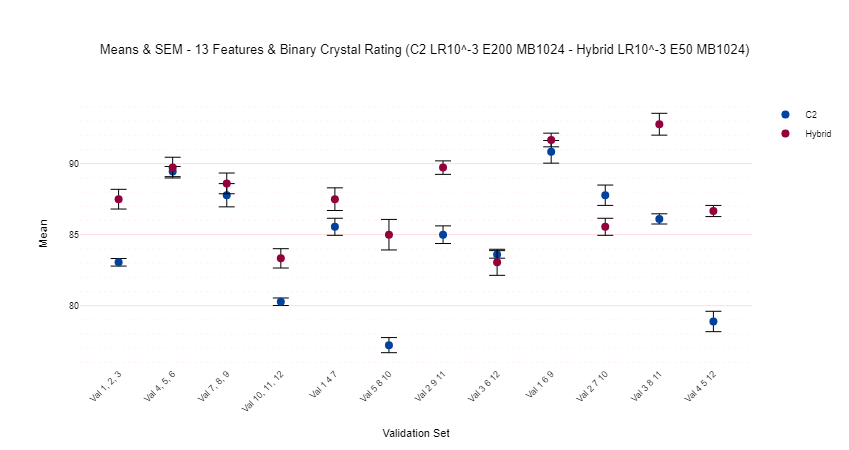
\includegraphics[width=0.85\textwidth, trim = 0.5cm 0cm 0.5cm 3.5cm, clip]{images/Means & SEM - 13 Features & Binary Crystal Rating (C2 LR10^-3 E200 MB1024 - Hybrid LR10^-3 E50 MB1024).png}
    \caption{Means and Standard Error of the Mean (SEM) Between Validation Sets - Analysis and Visualisation coded in Jupyter Notebooks using Plotly for Visualisation} \label{fig:Means and Standard Error of the Mean (SEM) Between Validation Sets - Analysis and Visualisation coded in Jupyter Notebooks using Plotly for Visualisation}
\end{figure}

% trim=left bottom right top

\subsection{Comparing the Accuracy of Rock Predictions - Hybrid - Continuous vs Binary Crystal Ratings}
\begin{figure}[H]
  \centering
    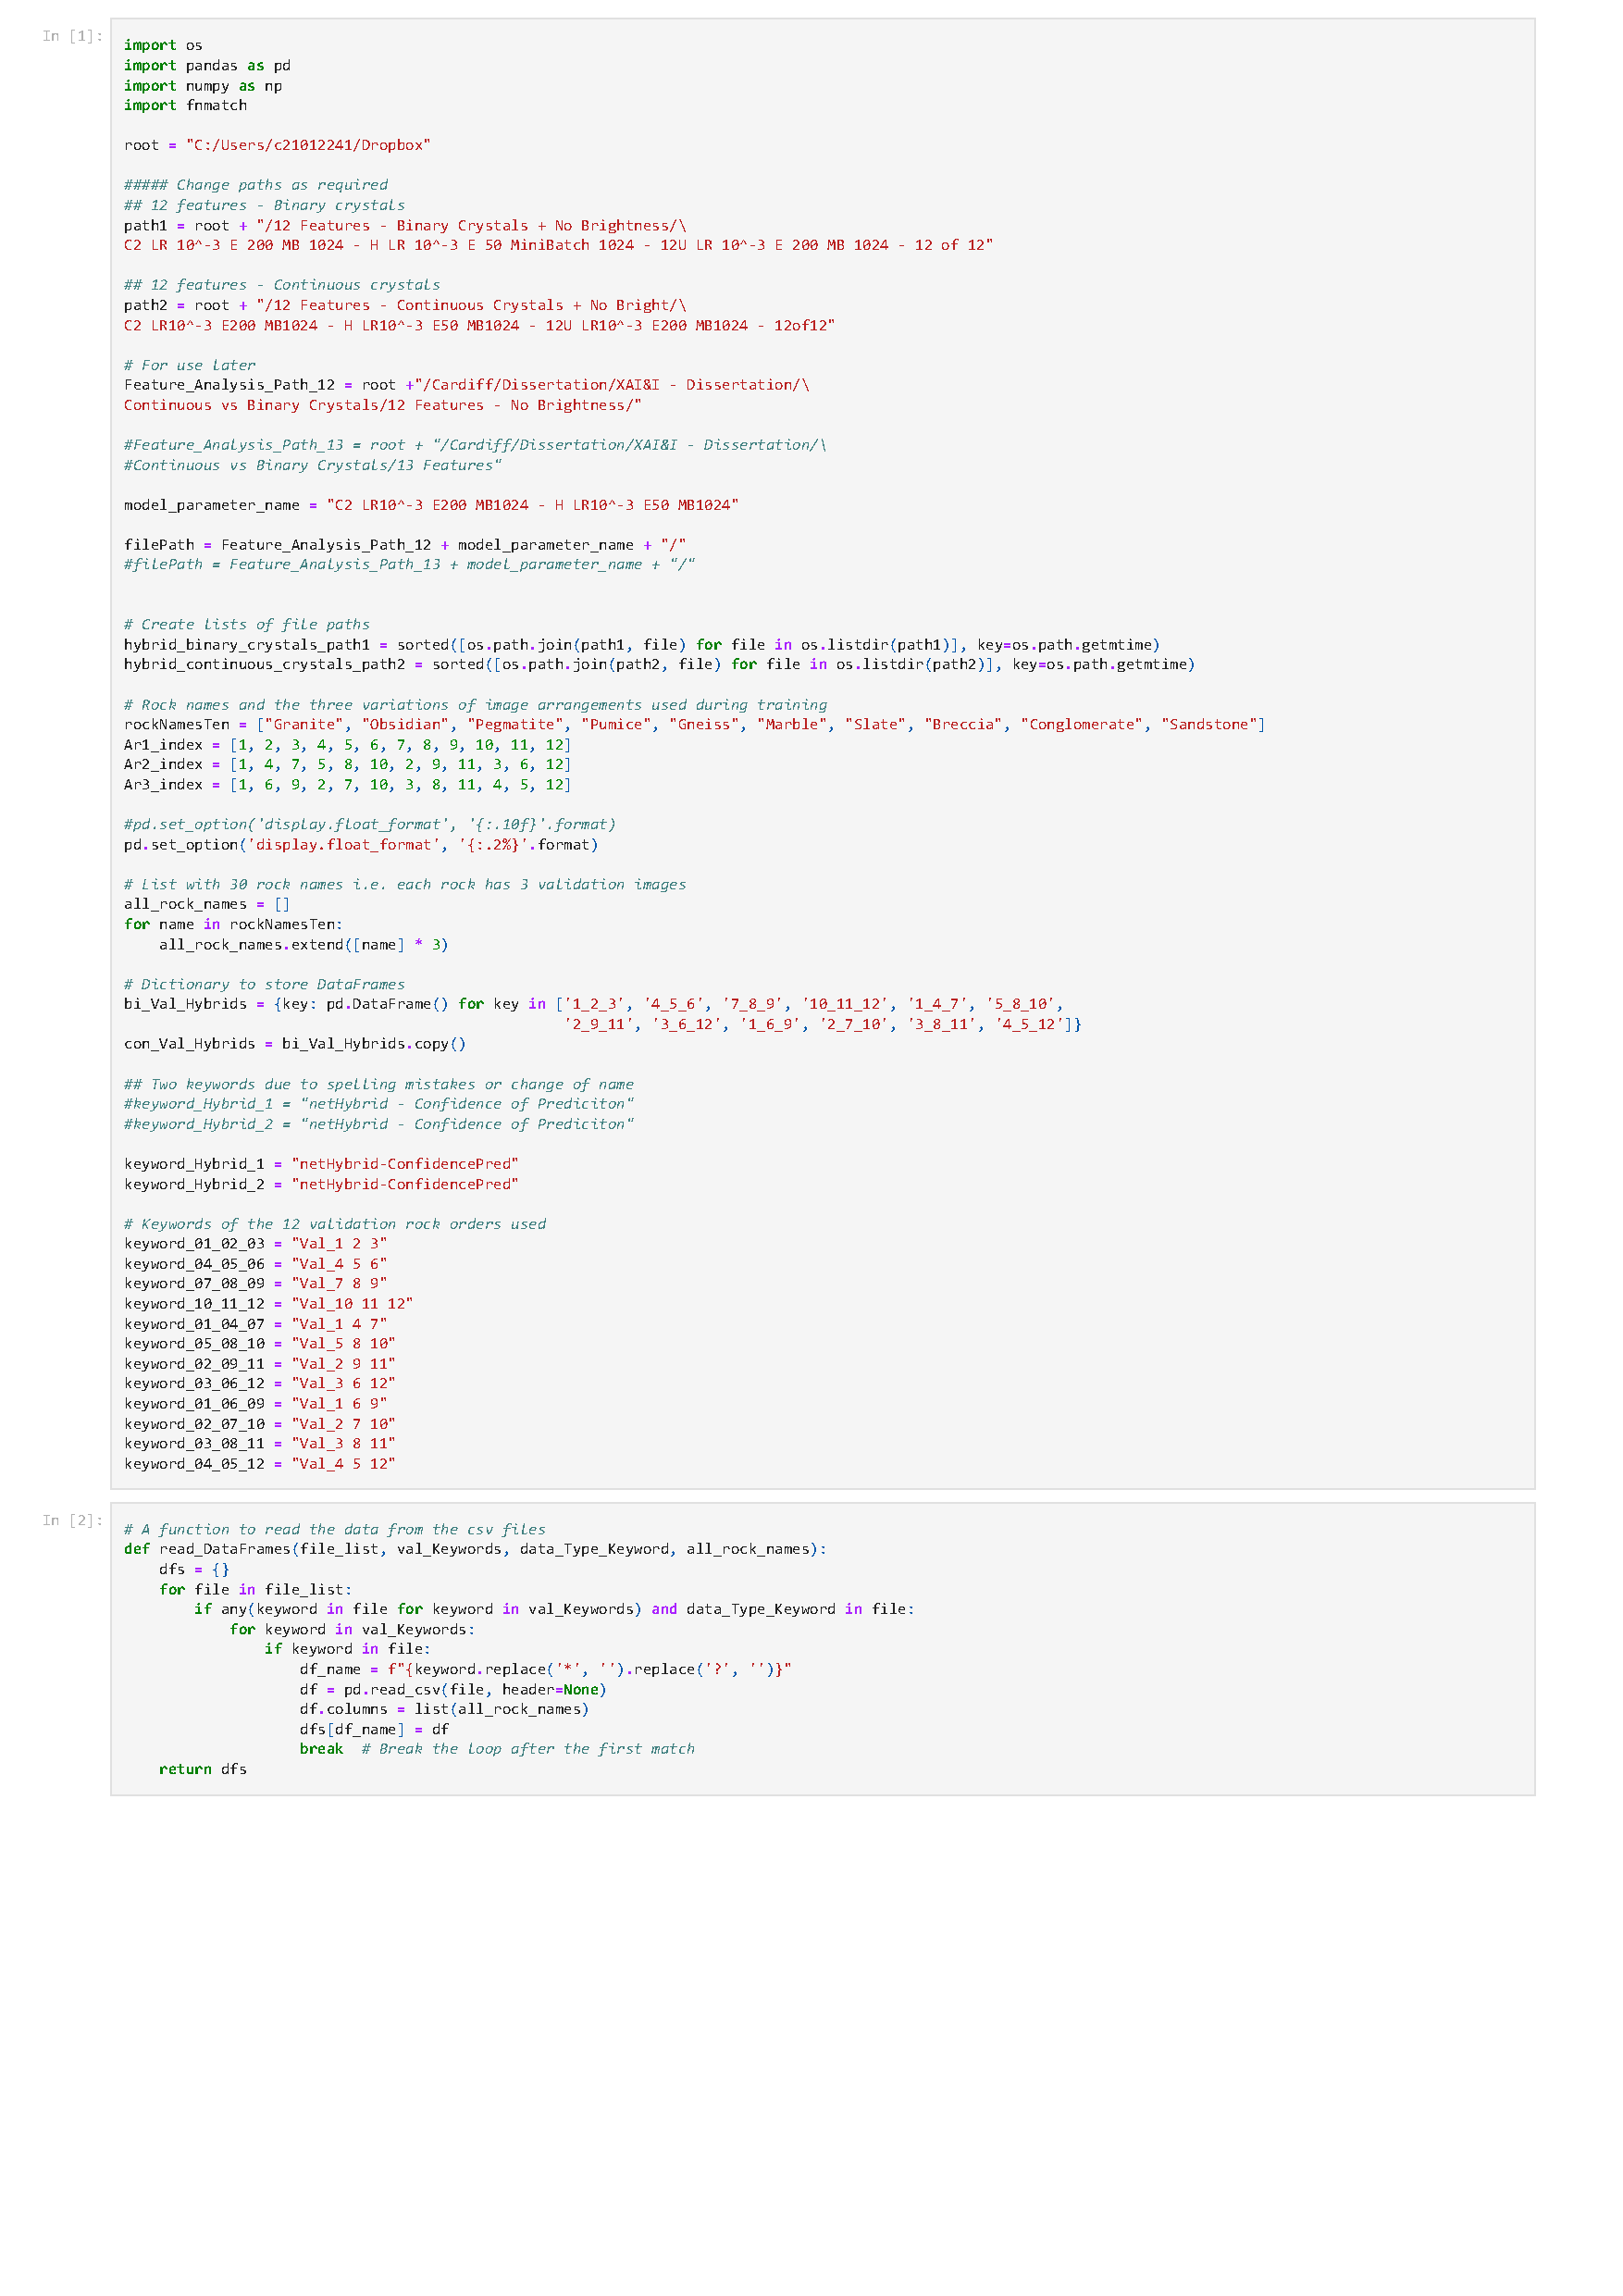
\includegraphics[width=0.9\textwidth, height=0.9\textheight]{Code/Compare2HybridModels V7.pdf}
\end{figure}
\includepdf[pages=2-5, width=0.9\textwidth, height=0.9\textheight]{Code/Compare2HybridModels V7.pdf}
%\includepdf[pages=6, width=0.9\textwidth, height=0.9\textheight, pagecommand={\null\vfill\captionof{lstlisting}{Comparing the Accuracy of Rock Predictions - Hybrid - Continuous vs Binary Crystal Ratings}}]{Code/Compare2HybridModels V7.pdf}
\begin{figure}[H]
  \centering
    \includegraphics[page=6, width=0.85\textwidth, trim= 20 100 20 10, clip]{Code/Compare2HybridModels V7.pdf}
    \caption{Comparing the Accuracy of Rock Predictions - Hybrid - Continuous vs Binary Crystal Ratings} \label{fig:Comparing the Accuracy of Rock Predictions - Hybrid - Continuous vs Binary Crystal Ratings}
\end{figure}



\section{Data Visualisations} \label{Data Visualisations}

\subsection{13 Features - Binary Crystal Rating} 

\begin{figure}[H]
  \centering
    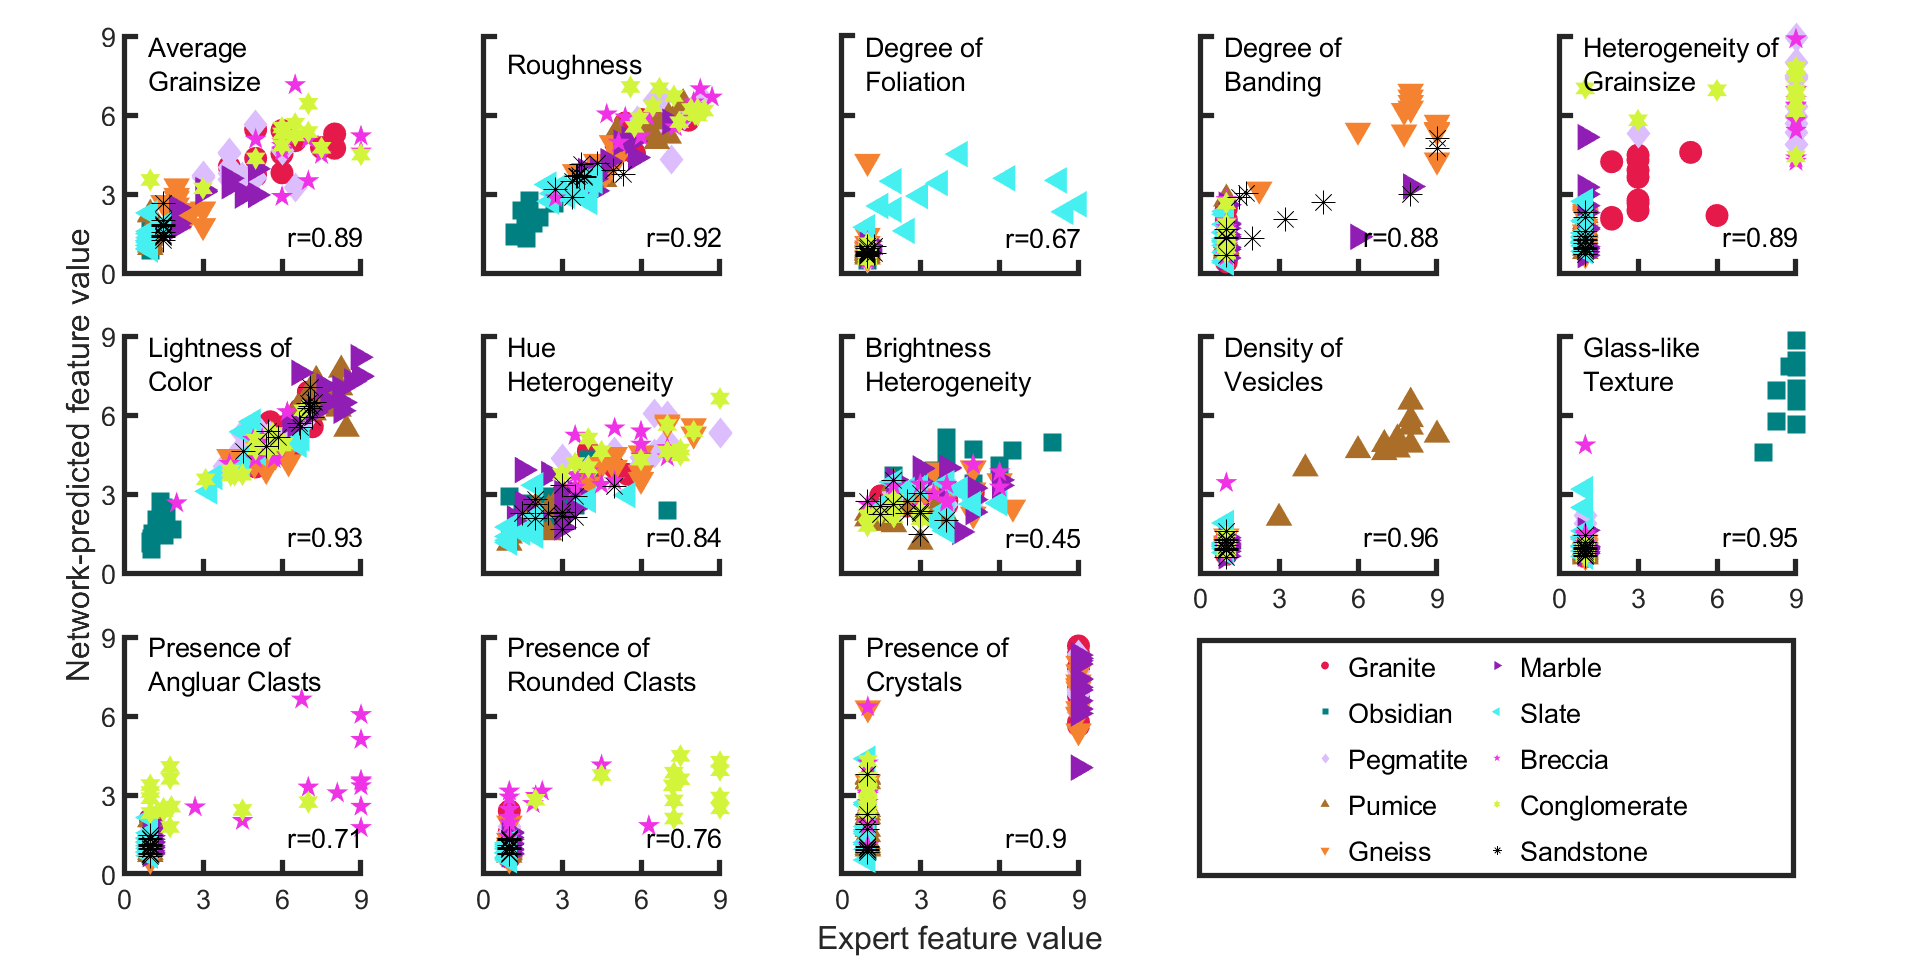
\includegraphics[width=\textwidth]{images/MATLAB Correlation - C2_Vs_Expert - 13 Feautres - Binary.png}
    \caption{Feature Correlation - Sequential CBM Vs Expert Ratings - 13 Features - Binary Crystal Rating} \label{fig:Feature Correlation - Sequential CBM Vs Expert Ratings - 13 Features - Binary Crystal Rating}
\end{figure}

\begin{figure}[H]
  \centering
    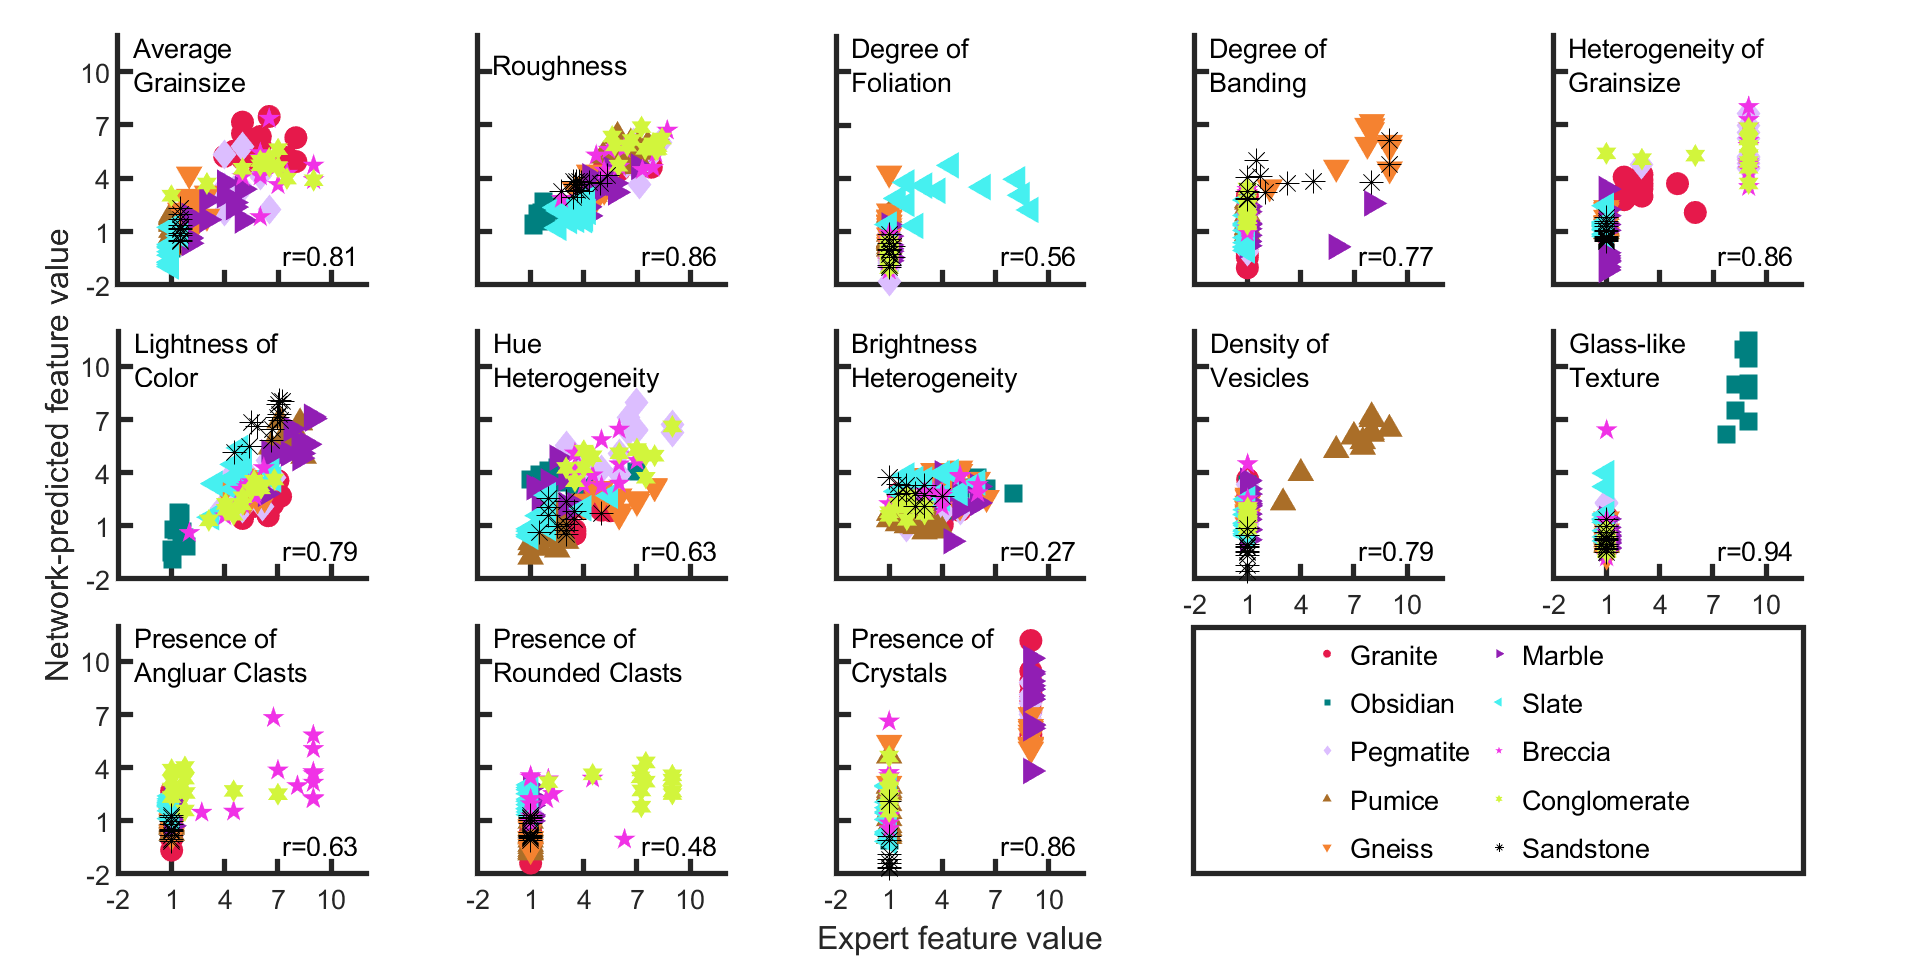
\includegraphics[width=\textwidth]{images/MATLAB Correlation - Hybrid_Vs_Expert - 13 Feautres - Binary.png}
    \caption{Feature Correlation - Hybrid Sequential CBM Vs Expert Ratings - 13 Features - Binary Crystal Rating} \label{fig:Feature Correlation - Hybrid Sequential CBM Vs Expert Ratings - 13 Features - Binary Crystal Rating}
\end{figure}

\begin{figure}[H]
  \centering
    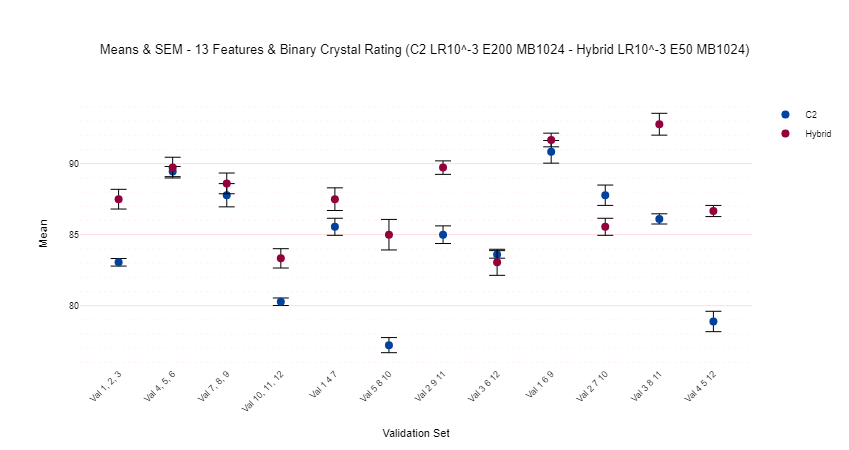
\includegraphics[width=\textwidth]{images/Means & SEM - 13 Features & Binary Crystal Rating (C2 LR10^-3 E200 MB1024 - Hybrid LR10^-3 E50 MB1024).png}
    \caption{Means \& SEM - Validation Sets - 13 Features - Binary Crystal Rating} \label{fig:Means & SEM - Validation Sets - 13 Features - Binary Crystal Rating}
\end{figure}


\begin{figure}[H]
  \centering
    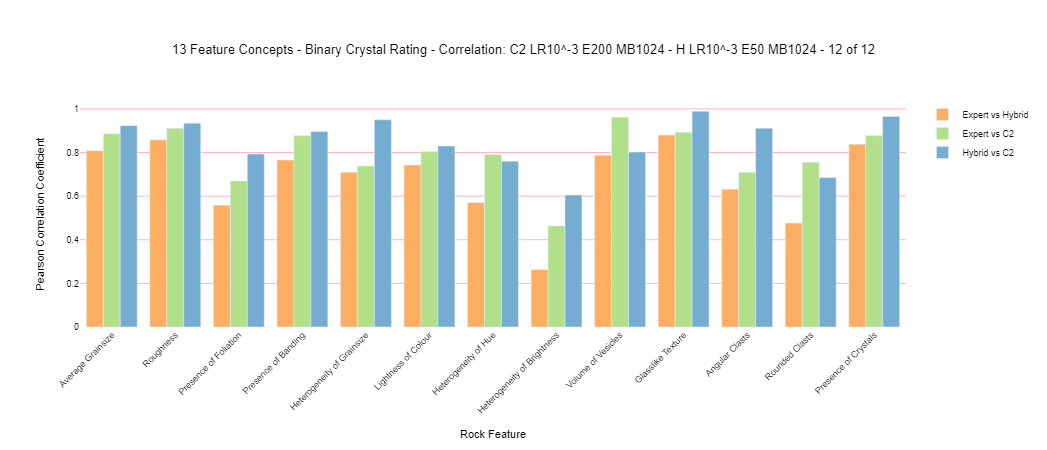
\includegraphics[width=\textwidth]{images/13 Feature Concepts - Binary Crystal Rating - Correlation- C2 LR10^-3 E200 MB1024 - H LR10^-3 E50 MB1024 - 12 of 12.png}
    \caption{13 Feature Concepts - Binary Crystal Rating - Mean correlation of Feature Concepts} \label{fig:13 Feature Concepts - Binary Crystal Rating - Mean correlation of Feature Concepts}
\end{figure}

% trim=left bottom right top

\begin{figure}[H]
  \centering
    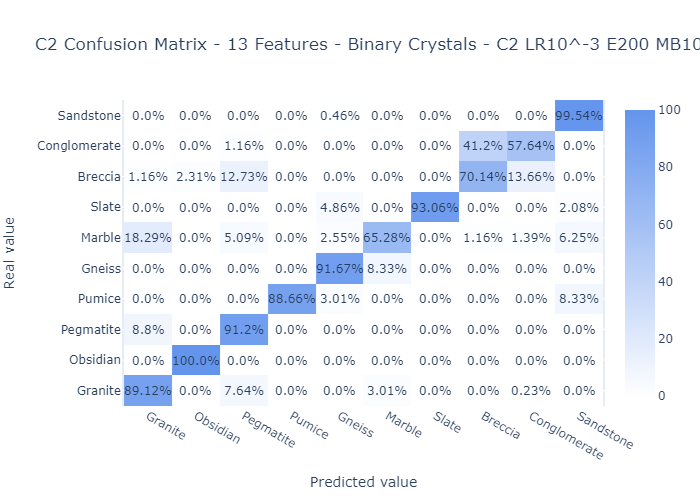
\includegraphics[width=0.9\textwidth, trim = 0cm 0cm 0.5cm 3.5cm, clip]{images/C2 Confusion Matrix - 13 Features - Binary Crystals.png}
    \caption{Sequential CBM Network Accuracy Confusion Matrix - 13 Features - Binary Crystal Ratings} \label{fig:Sequential CBM Network Accuracy Confusion Matrix - 13 Features - Binary Crystal Ratings}
\end{figure}

\begin{figure}[H]
  \centering
    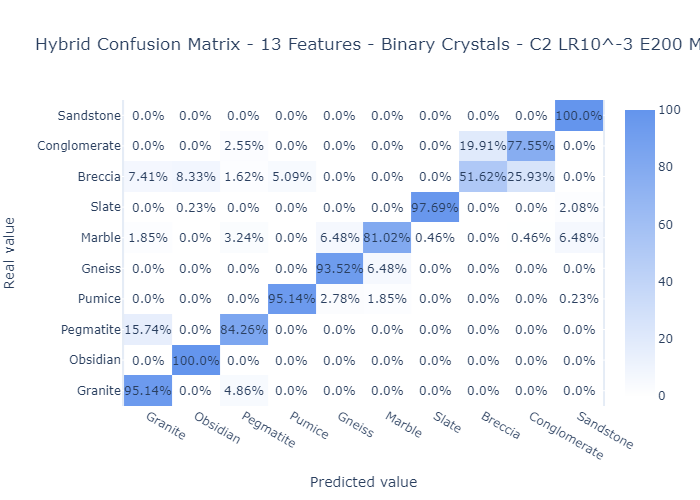
\includegraphics[width=0.9\textwidth, trim = 0cm 0cm 0.5cm 3.5cm, clip]{images/Hybrid Confusion Matrix- 13 Features - Binary Crystals.png}
    \caption{Hybrid Network Accuracy Confusion Matrix - 13 Features - Binary Crystal Ratings} \label{fig:Hybrid Network Accuracy -  13 Features - Binary Crystal Ratings - Confusion Matrix}
\end{figure}

\subsection{13 Features - Continuous Crystal Rating}

\begin{figure}[H]
  \centering
    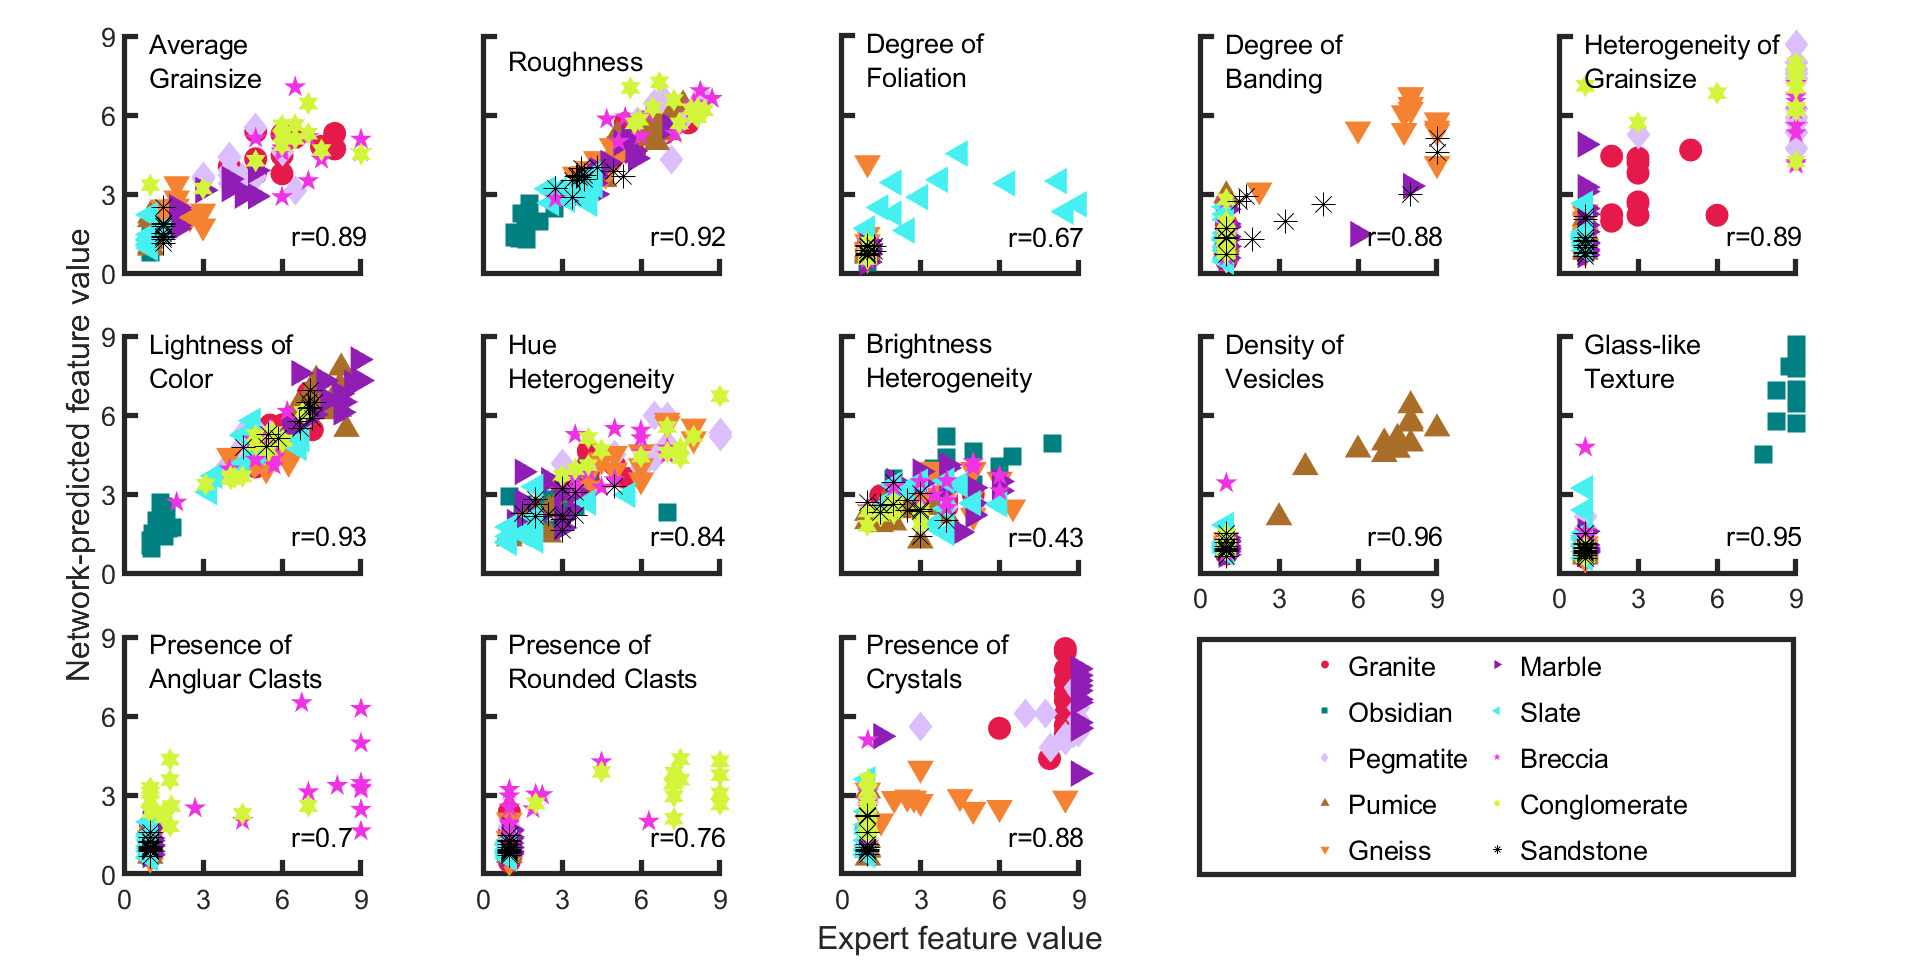
\includegraphics[width=\textwidth]{images/MATLAB Correlation - C2_Vs_Expert - 13 Feautres - Continuous.png}
    \caption{Feature Correlation - Sequential CBM Vs Expert Ratings - 13 Features - Continuous Crystal Rating} \label{fig:Feature Correlation - Sequential CBM Vs Expert Ratings - 13 Features - Continuous Crystal Rating}
\end{figure}

\begin{figure}[H]
  \centering
    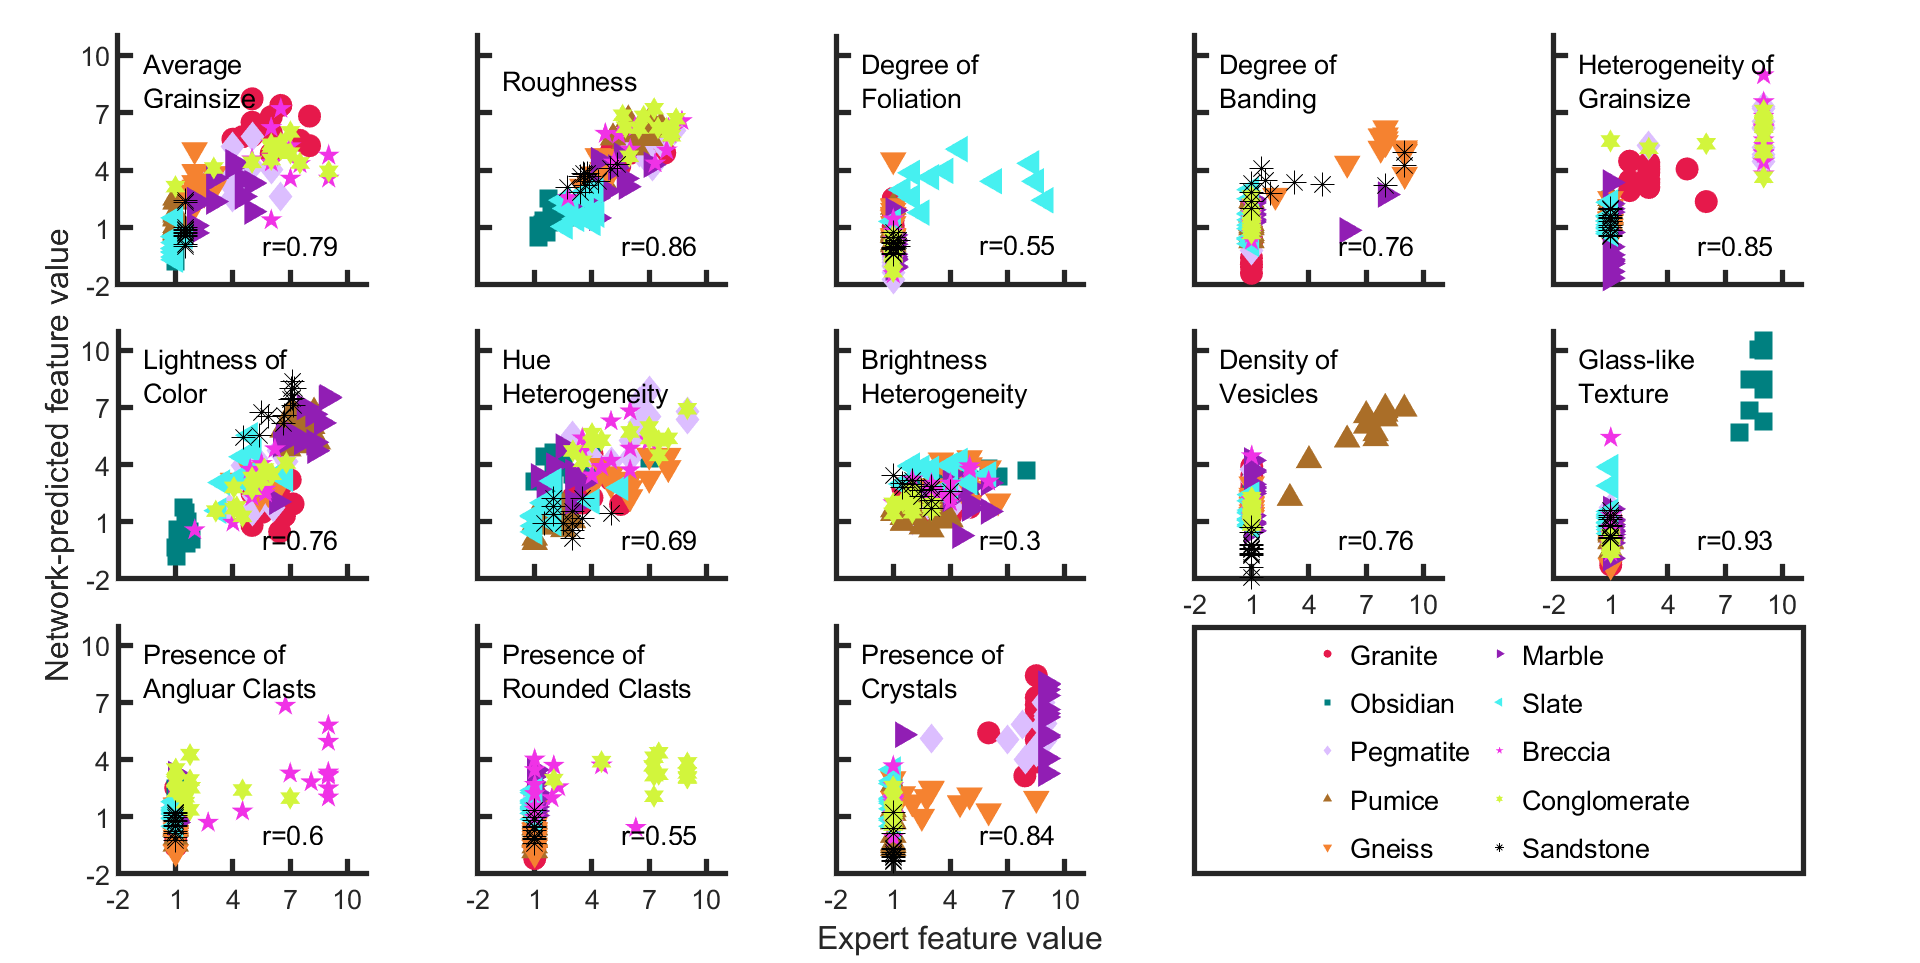
\includegraphics[width=\textwidth]{images/MATLAB Correlation - Hybrid_Vs_Expert - 13 Feautres - Continuous.png}
    \caption{Feature Correlation - Hybrid Sequential CBM Vs Expert Ratings - 13 Features - Continuous Crystal Rating} \label{fig:Feature Correlation - Hybrid Sequential CBM Vs Expert Ratings - 13 Features - Continuous Crystal Rating}
\end{figure}

\begin{figure}[H]
  \centering
    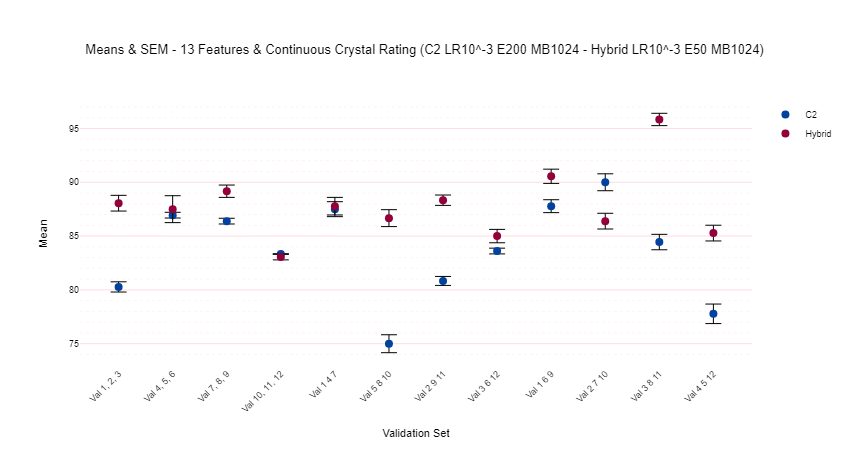
\includegraphics[width=\textwidth]{images/Means & SEM - 13 Features & Continuous Crystal Rating (C2 LR10^-3 E200 MB1024 - Hybrid LR10^-3 E50 MB1024).png}
    \caption{Means \& SEM - Validation Sets - 13 Features - Continuous Crystal Rating} \label{fig:Means & SEM - Validation Sets - 13 Features - Continuous Crystal Rating}
\end{figure}


\begin{figure}[H]
  \centering
    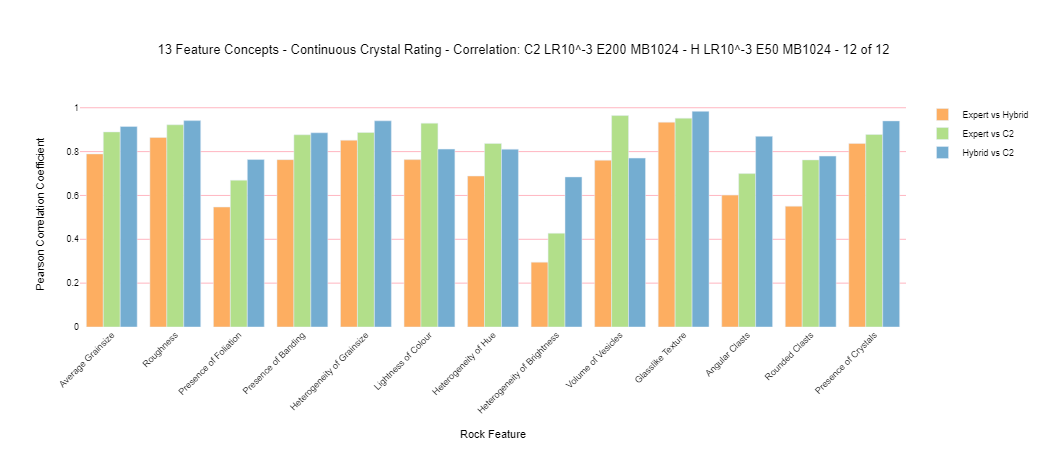
\includegraphics[width=\textwidth]{images/13 Feature Concepts - Continuous Crystal Rating - Correlation- C2 LR10^-3 E200 MB1024 - H LR10^-3 E50 MB1024 - 12 of 12.png}
    \caption{13 Feature Concepts - Continuous Crystal Rating - Mean correlation of Feature Concepts} \label{fig:13 Feature Concepts - Continuous Crystal Rating - Mean correlation of Feature Concepts}
\end{figure}


\begin{figure}[H]
  \centering
    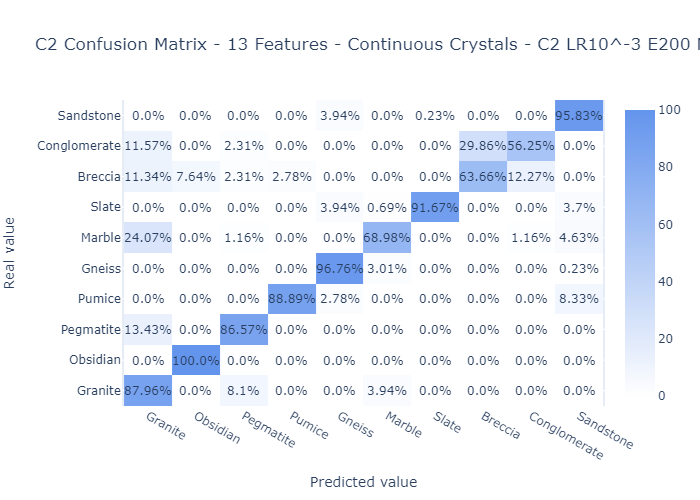
\includegraphics[width=0.9\textwidth, trim = 0cm 0cm 0.5cm 3.5cm, clip]{images/C2 Confusion Matrix - 13 Features - Continuous Crystals.png}
    \caption{Sequential CBM Network Accuracy Confusion Matrix - 13 Features - Continuous Crystal Ratings} \label{fig:Sequential CBM Network Accuracy Confusion Matrix - 13 Features - Continuous Crystal Ratings}
\end{figure}

\begin{figure}[H]
  \centering
    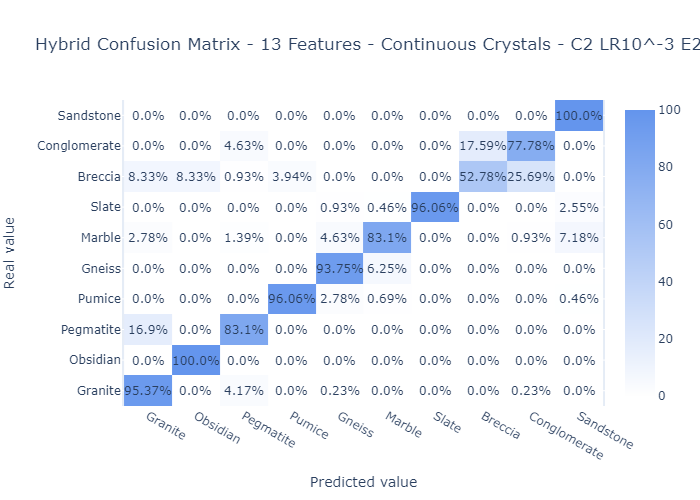
\includegraphics[width=0.9\textwidth, trim = 0cm 0cm 0.5cm 3.5cm, clip]{images/Hybrid Confusion Matrix - 13 Features - Continuous Crystals.png}
    \caption{Hybrid Network Accuracy Confusion Matrix- 13 Features - Continuous Crystal Ratings} \label{fig:Hybrid Network Accuracy Confusion Matrix- 13 Features - Continuous Crystal Ratings}
\end{figure}

\subsection{12 Features ("Heterogeneity of Brightness" Feature Removed) - Binary Crystal Rating}

\begin{figure}[H]
  \centering
    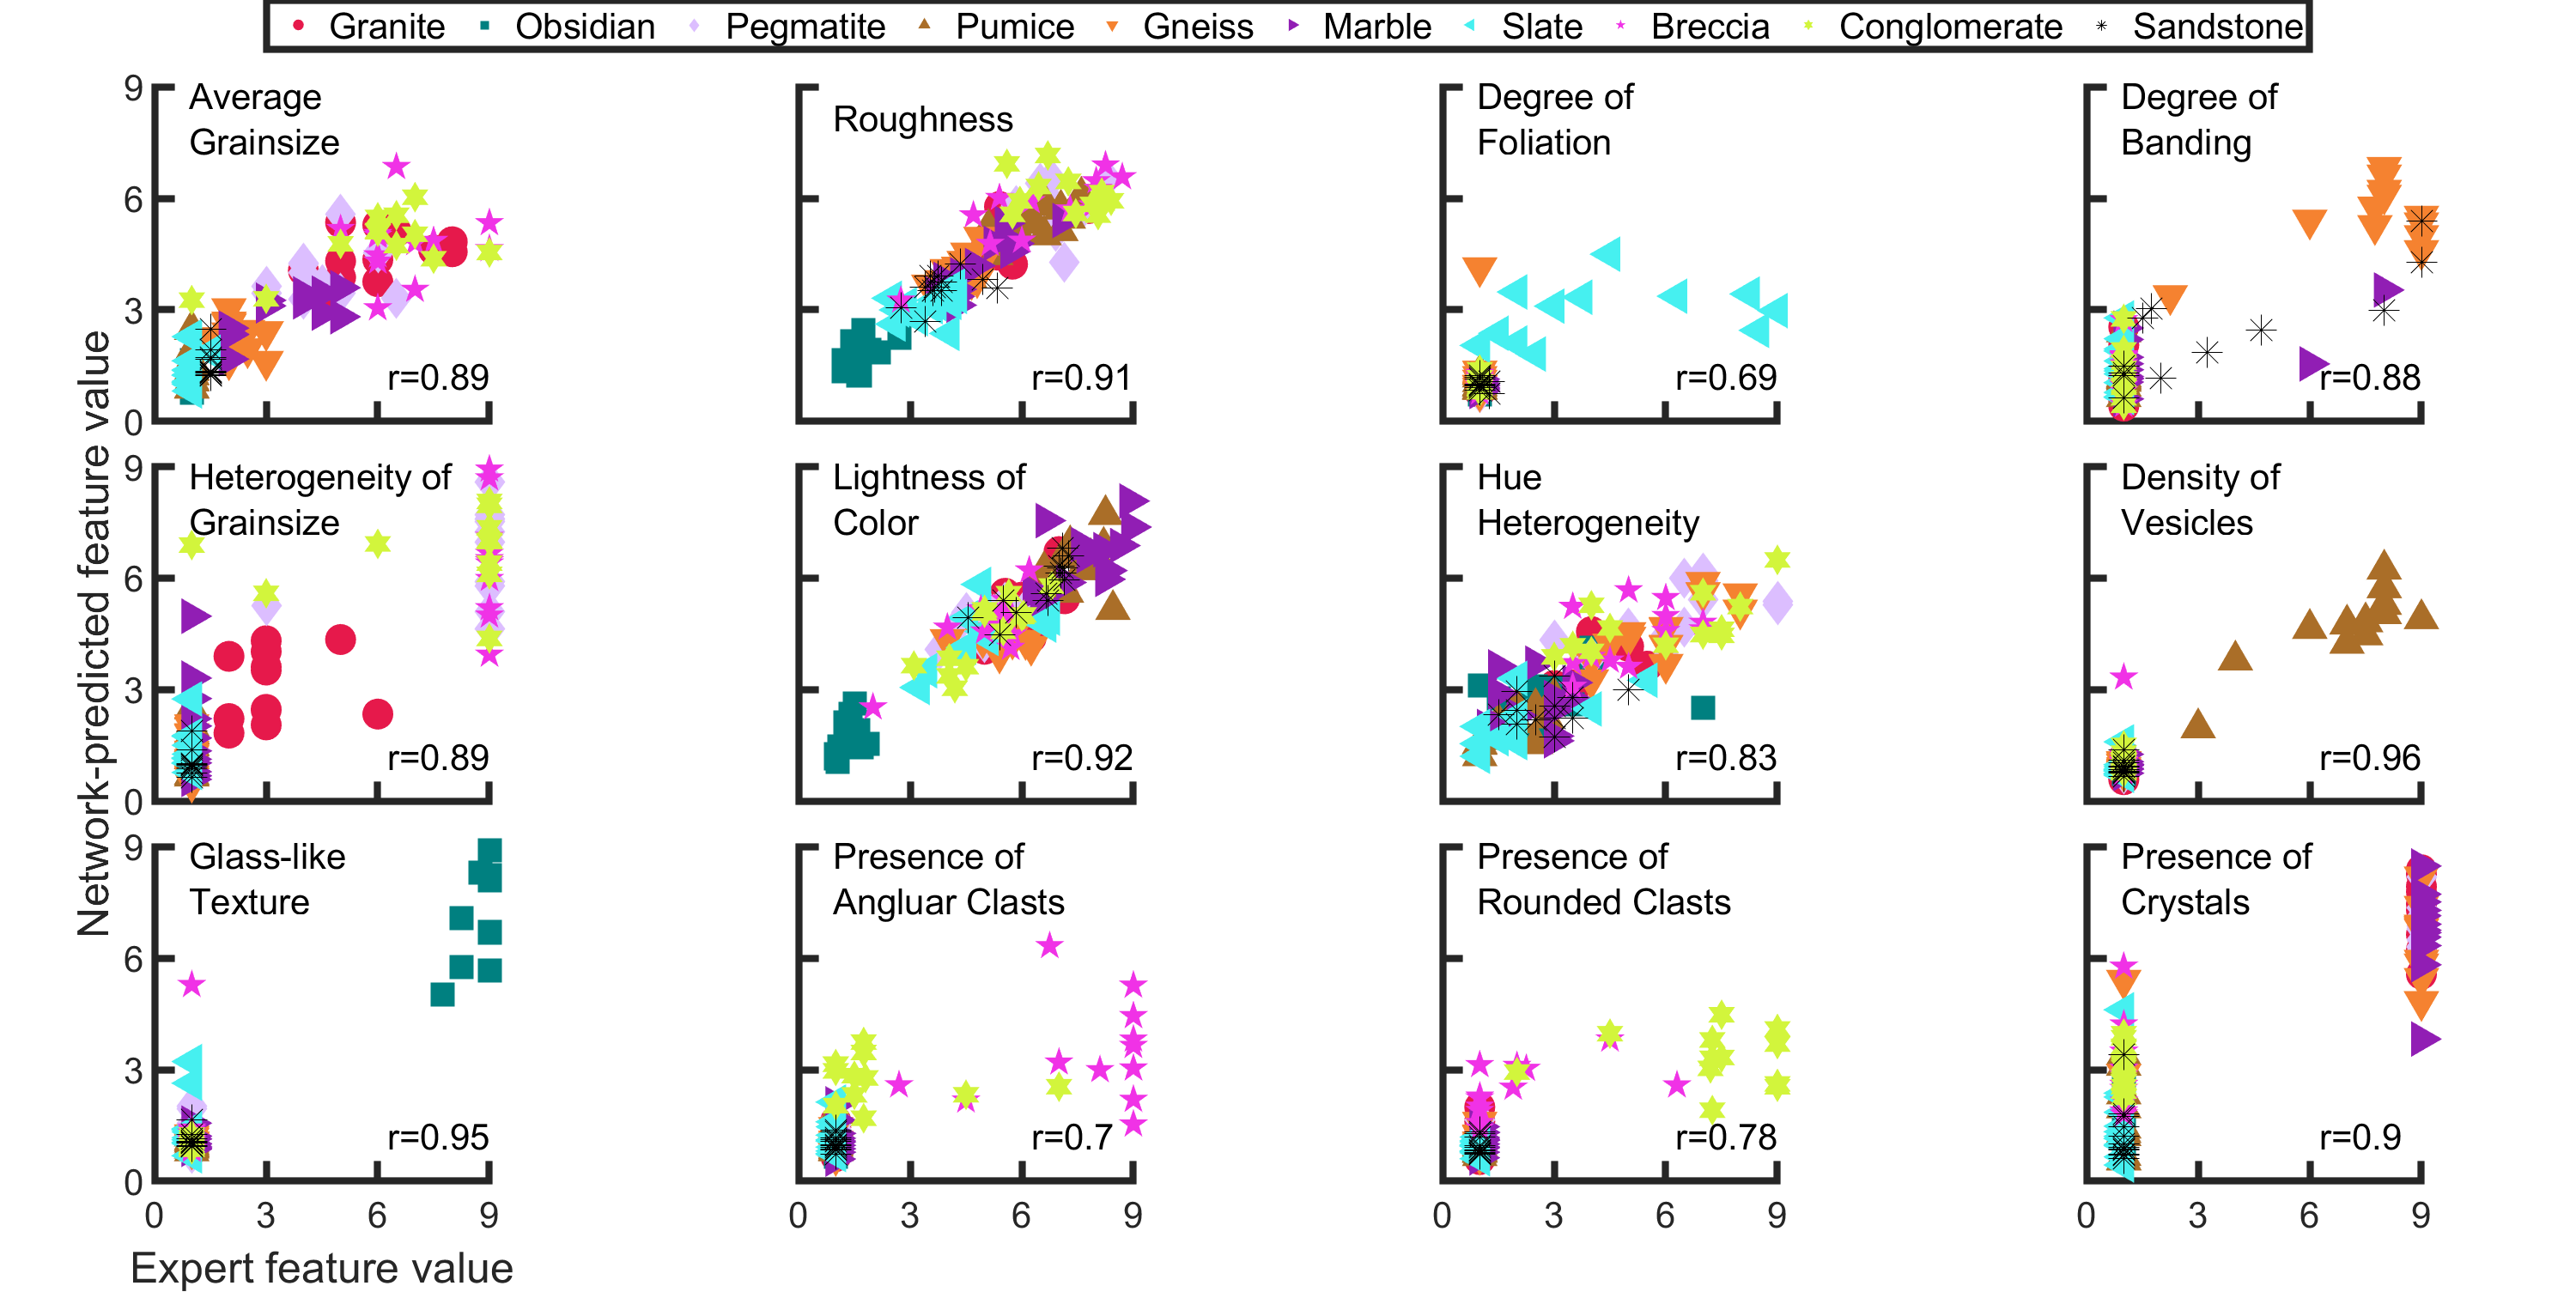
\includegraphics[width=\textwidth]{images/MATLAB Correlation - C2_Vs_Expert - 12 Feautres - Binary.png}
    \caption{Feature Correlation - Sequential CBM Vs Expert Ratings - 12 Features - Binary Crystal Rating} \label{fig:Feature Correlation - Sequential CBM Vs Expert Ratings - 12 Features - Binary Crystal Rating}
\end{figure}

\begin{figure}[H]
  \centering
    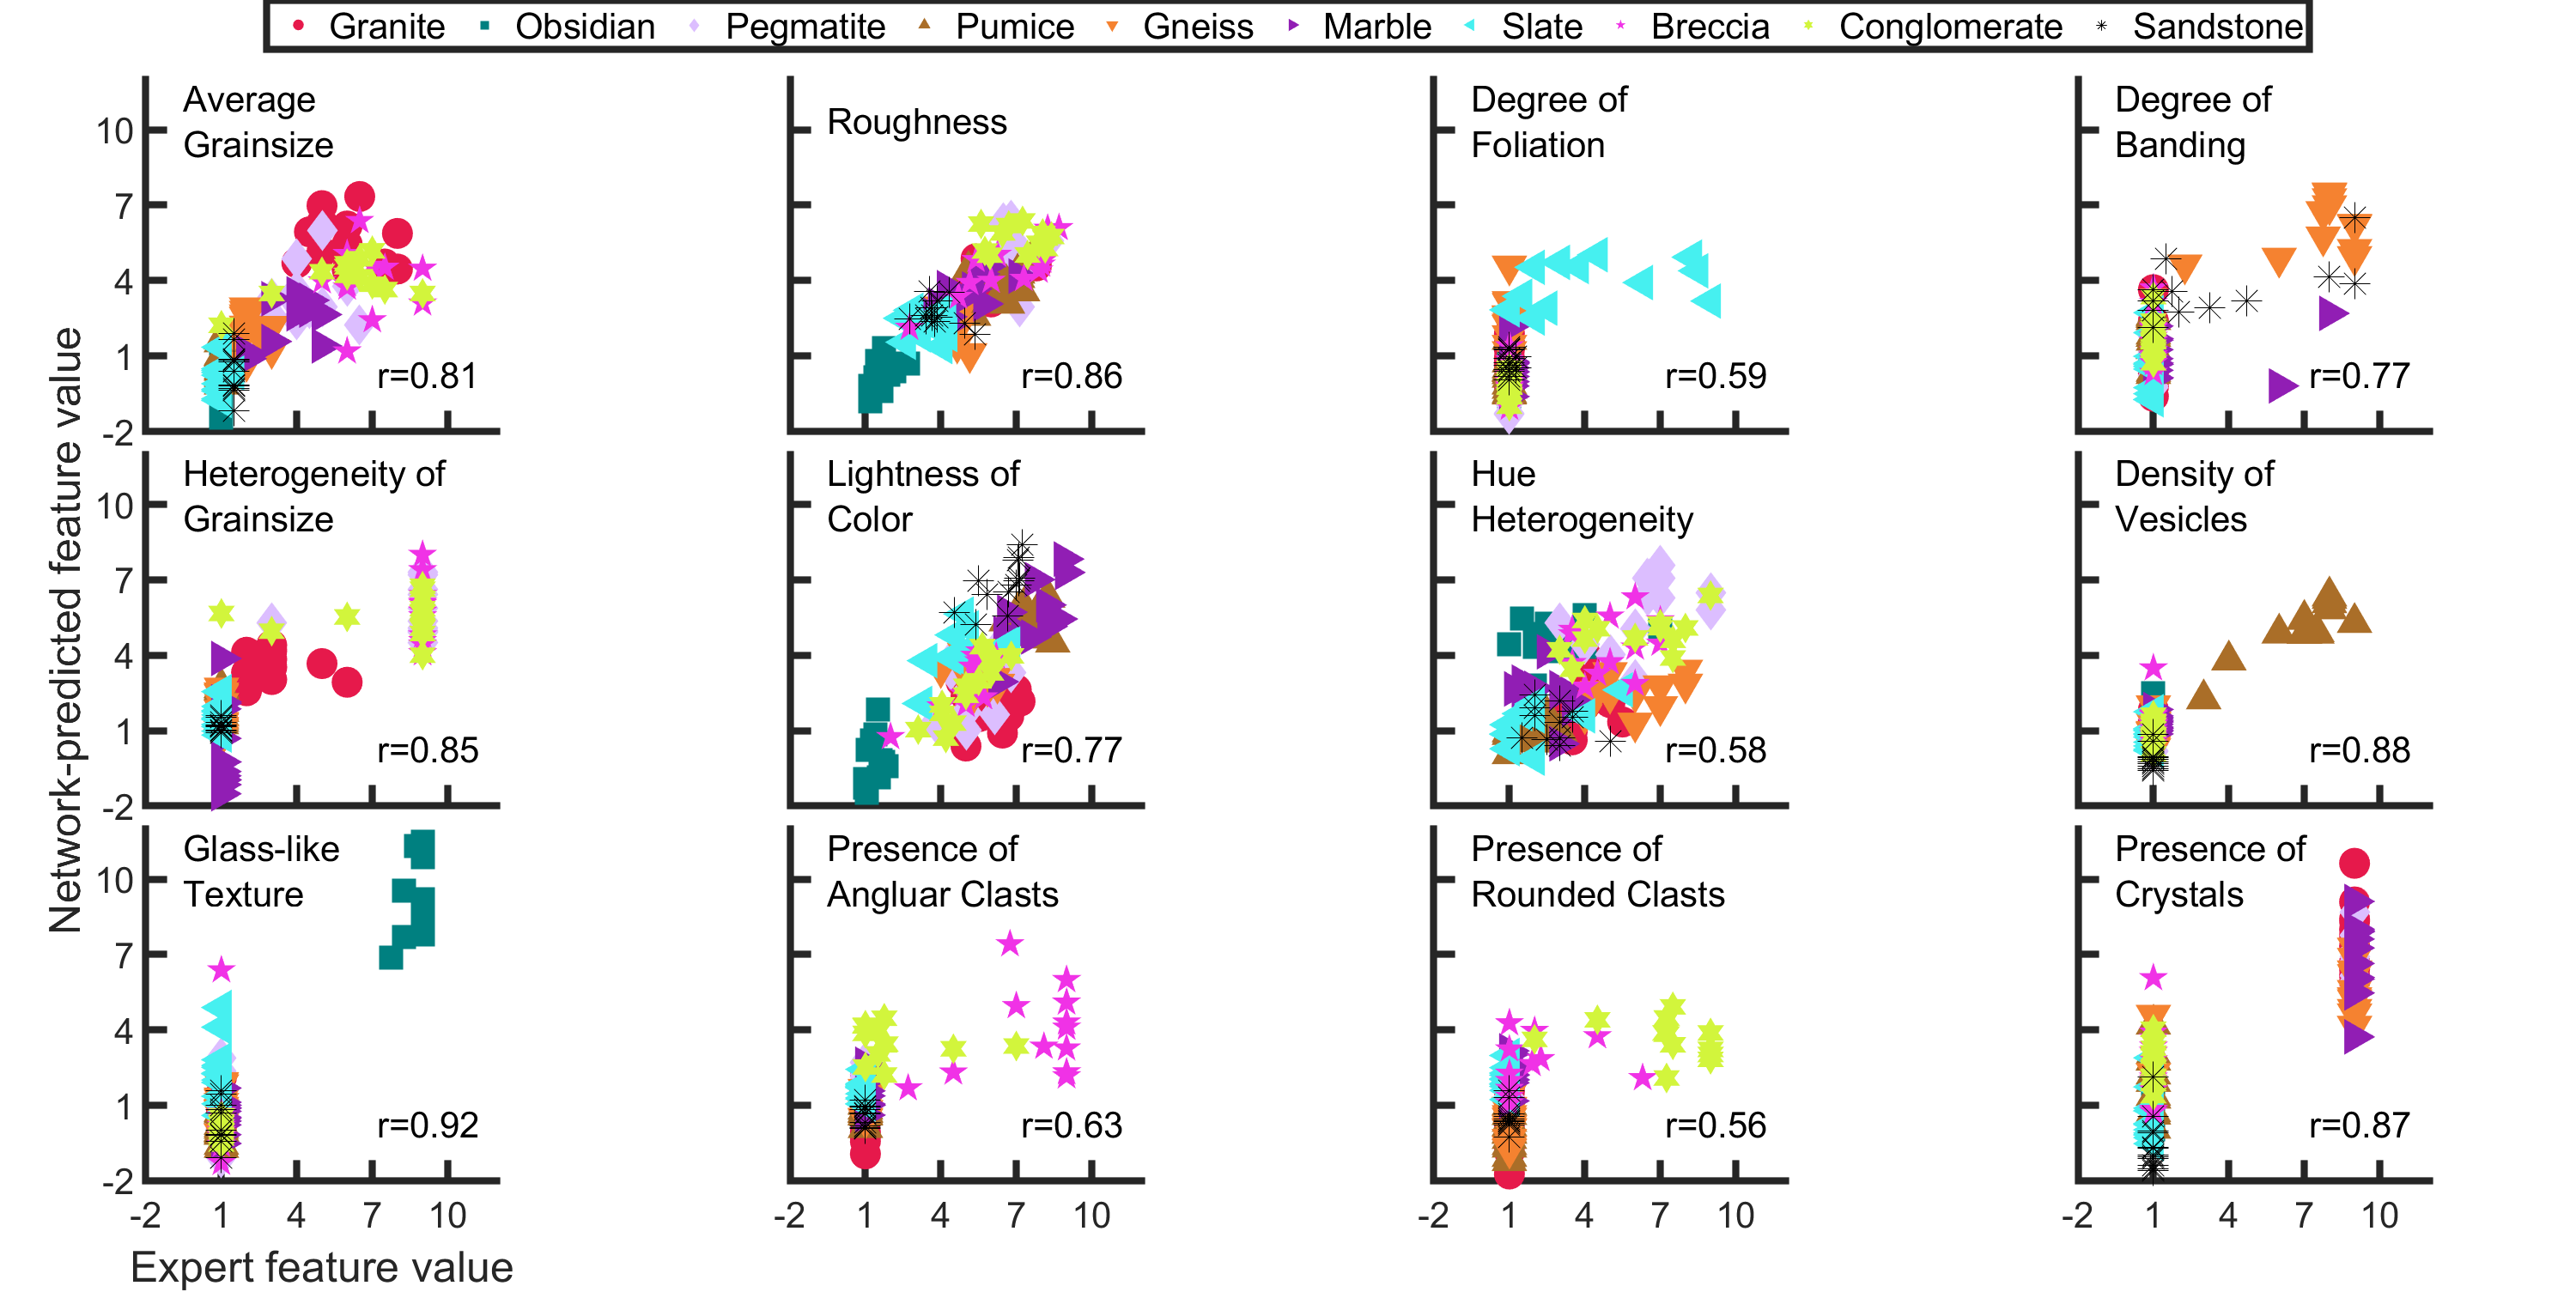
\includegraphics[width=\textwidth]{images/MATLAB Correlation - Hybrid_Vs_Expert - 12 Feautres - Binary.png}
    \caption{Feature Correlation - Hybrid Sequential CBM Vs Expert Ratings - 12 Features - Binary Crystal Rating} \label{fig:Feature Correlation - Hybrid Sequential CBM Vs Expert Ratings - 12 Features - Binary Crystal Rating}
\end{figure}

\begin{figure}[H]
  \centering
    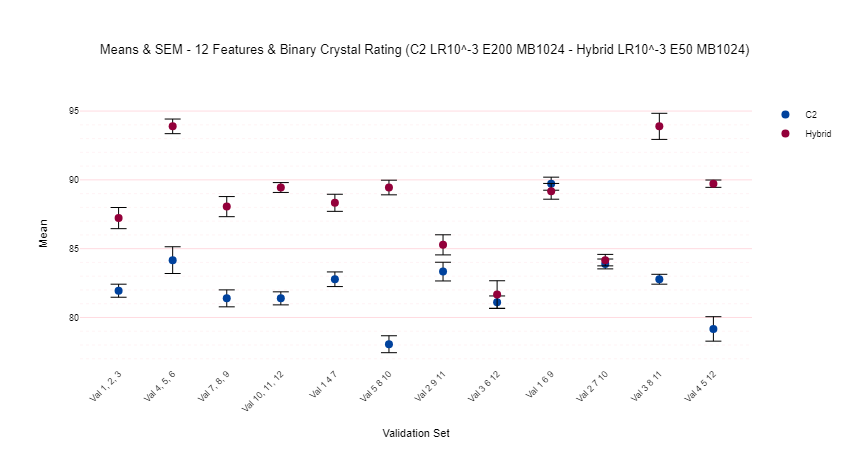
\includegraphics[width=\textwidth]{images/Means & SEM - 12 Features & Binary Crystal Rating (C2 LR10^-3 E200 MB1024 - Hybrid LR10^-3 E50 MB1024).png}
    \caption{Means \& SEM - Validation Sets - 12 Features - Binary Crystal Rating} \label{fig:Means & SEM - Validation Sets - 12 Features - Binary Crystal Rating}
\end{figure}


\begin{figure}[H]
  \centering
    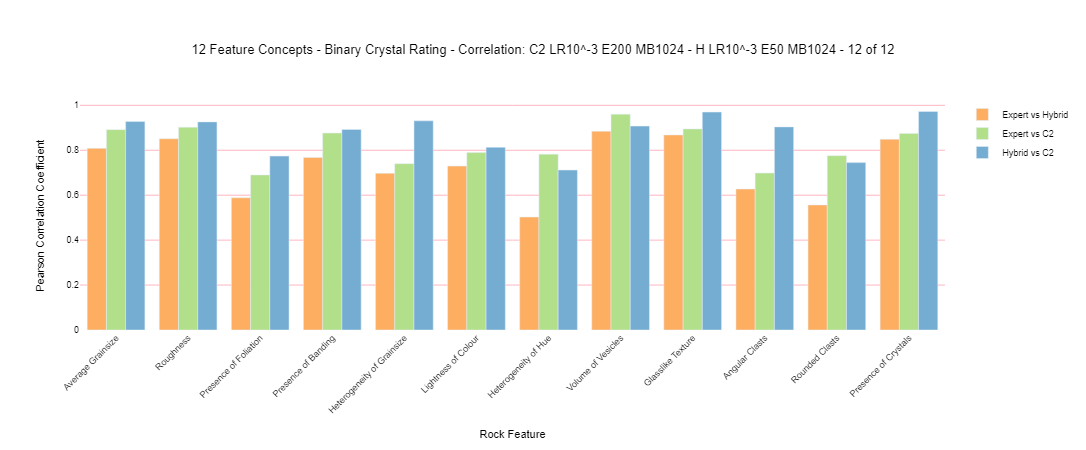
\includegraphics[width=\textwidth]{images/12 Feature Concepts - Binary Crystal Rating - Correlation- C2 LR10^-3 E200 MB1024 - H LR10^-3 E50 MB1024 - 12 of 12.png}
    \caption{12 Feature Concepts - Binary Crystal Rating - Mean correlation of Feature Concepts} \label{fig:12 Feature Concepts - Binary Crystal Rating - Mean correlation of Feature Concepts}
\end{figure}

\begin{figure}[H]
  \centering
    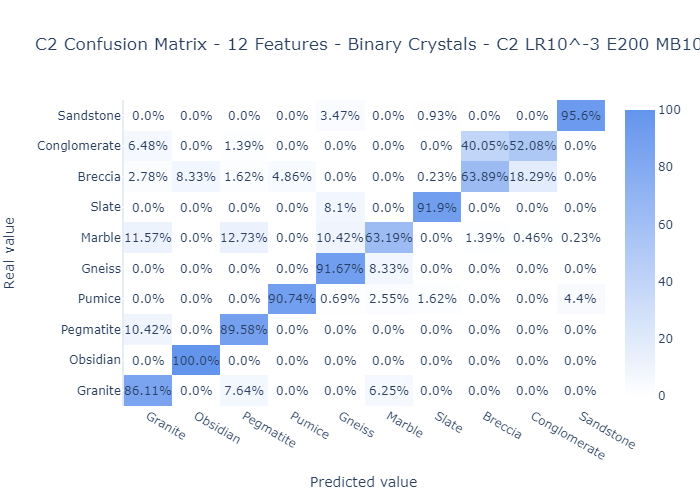
\includegraphics[width=0.9\textwidth, trim = 0cm 0cm 0.5cm 3.5cm, clip]{images/C2 Confusion Matrix - 12 Features - Binary Crystals.png}
    \caption{Sequential CBM Network Accuracy Confusion Matrix - 12 Features - Binary Crystal Ratings} \label{fig:Sequential CBM Network Accuracy Confusion Matrix - 12 Features - Binary Crystal Ratings}
\end{figure}

\begin{figure}[H]
  \centering
    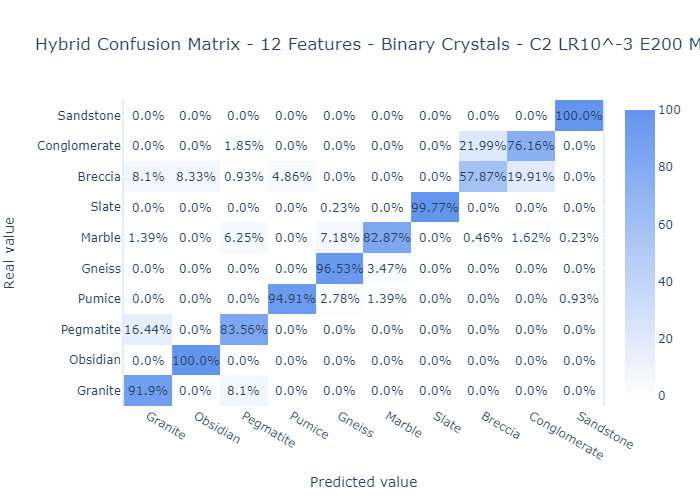
\includegraphics[width=0.9\textwidth, trim = 0cm 0cm 0.5cm 3.5cm, clip]{images/Hybrid Confusion Matrix - 12 Features - Binary Crystals.png }
    \caption{Hybrid Network Accuracy Confusion Matrix - 12 Features - Binary Crystal Ratings} \label{fig:Hybrid Network Accuracy Confusion Matrix- 12 Features - Binary Crystal Ratings}
\end{figure}

\subsection{12 Features ("Heterogeneity of Brightness" Feature Removed) - Continuous Crystal Rating}

\begin{figure}[H]
  \centering
    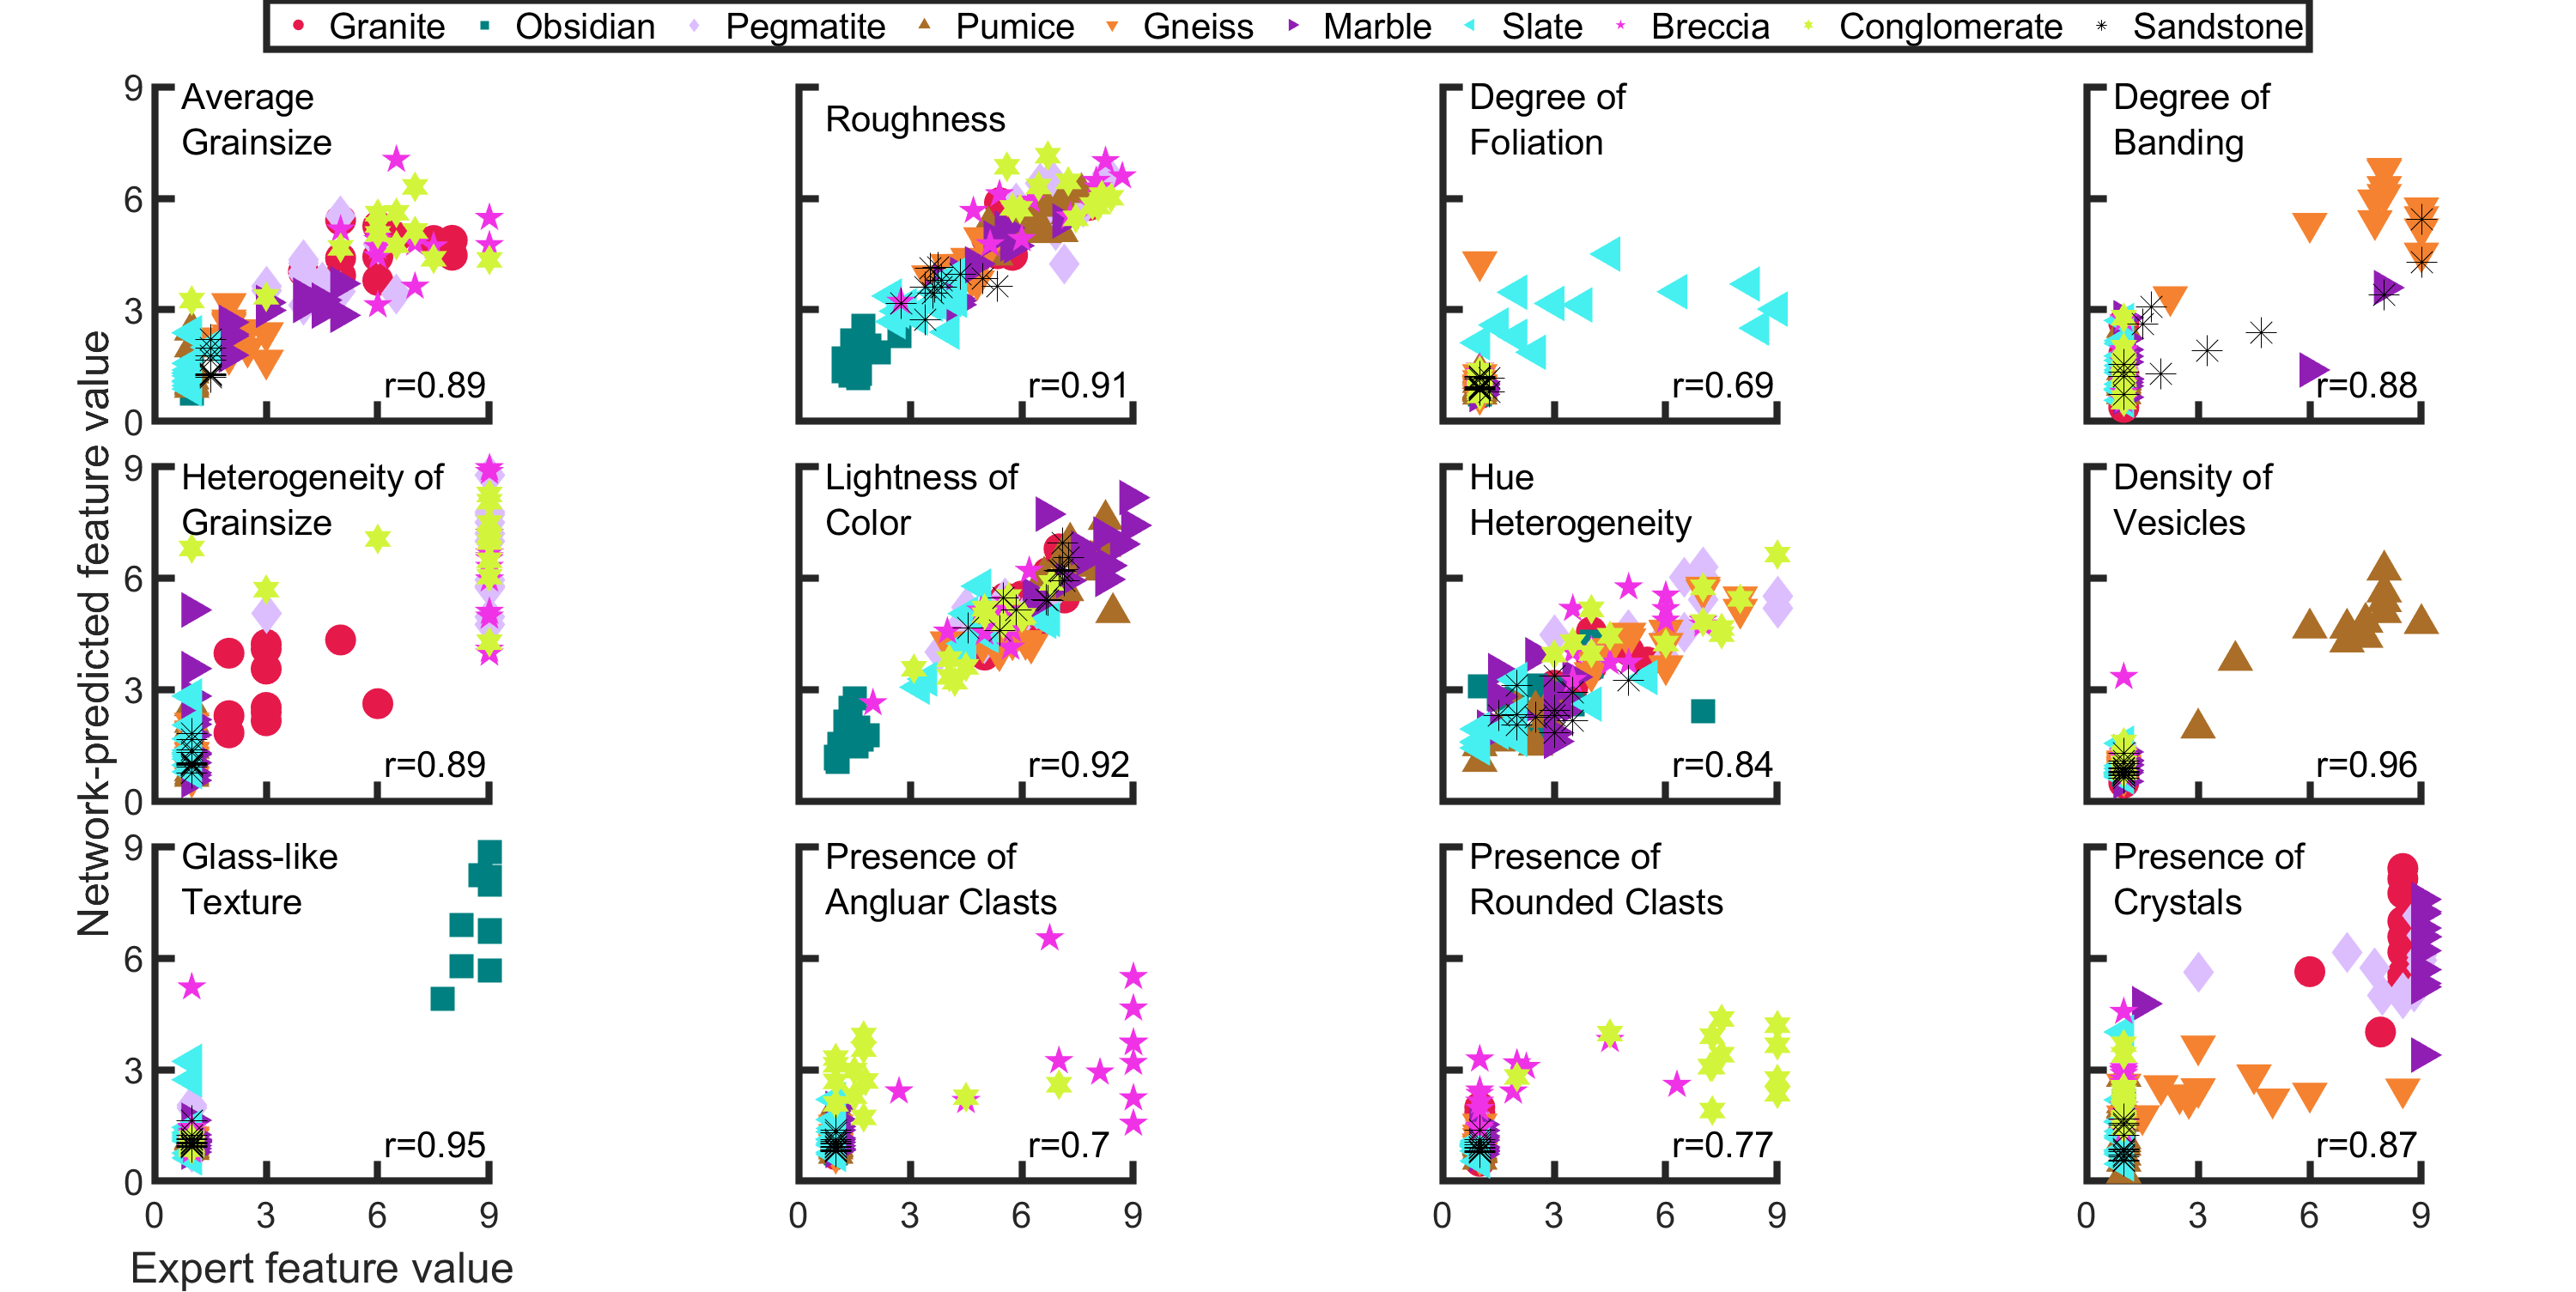
\includegraphics[width=\textwidth]{images/MATLAB Correlation - C2_Vs_Expert - 12 Feautres - Continuous.png}
    \caption{Feature Correlation - Sequential CBM Vs Expert Ratings - 12 Features - Continuous Crystal Rating} \label{fig:Feature Correlation - Sequential CBM Vs Expert Ratings - 12 Features - Continuous Crystal Rating}
\end{figure}

\begin{figure}[H]
  \centering
    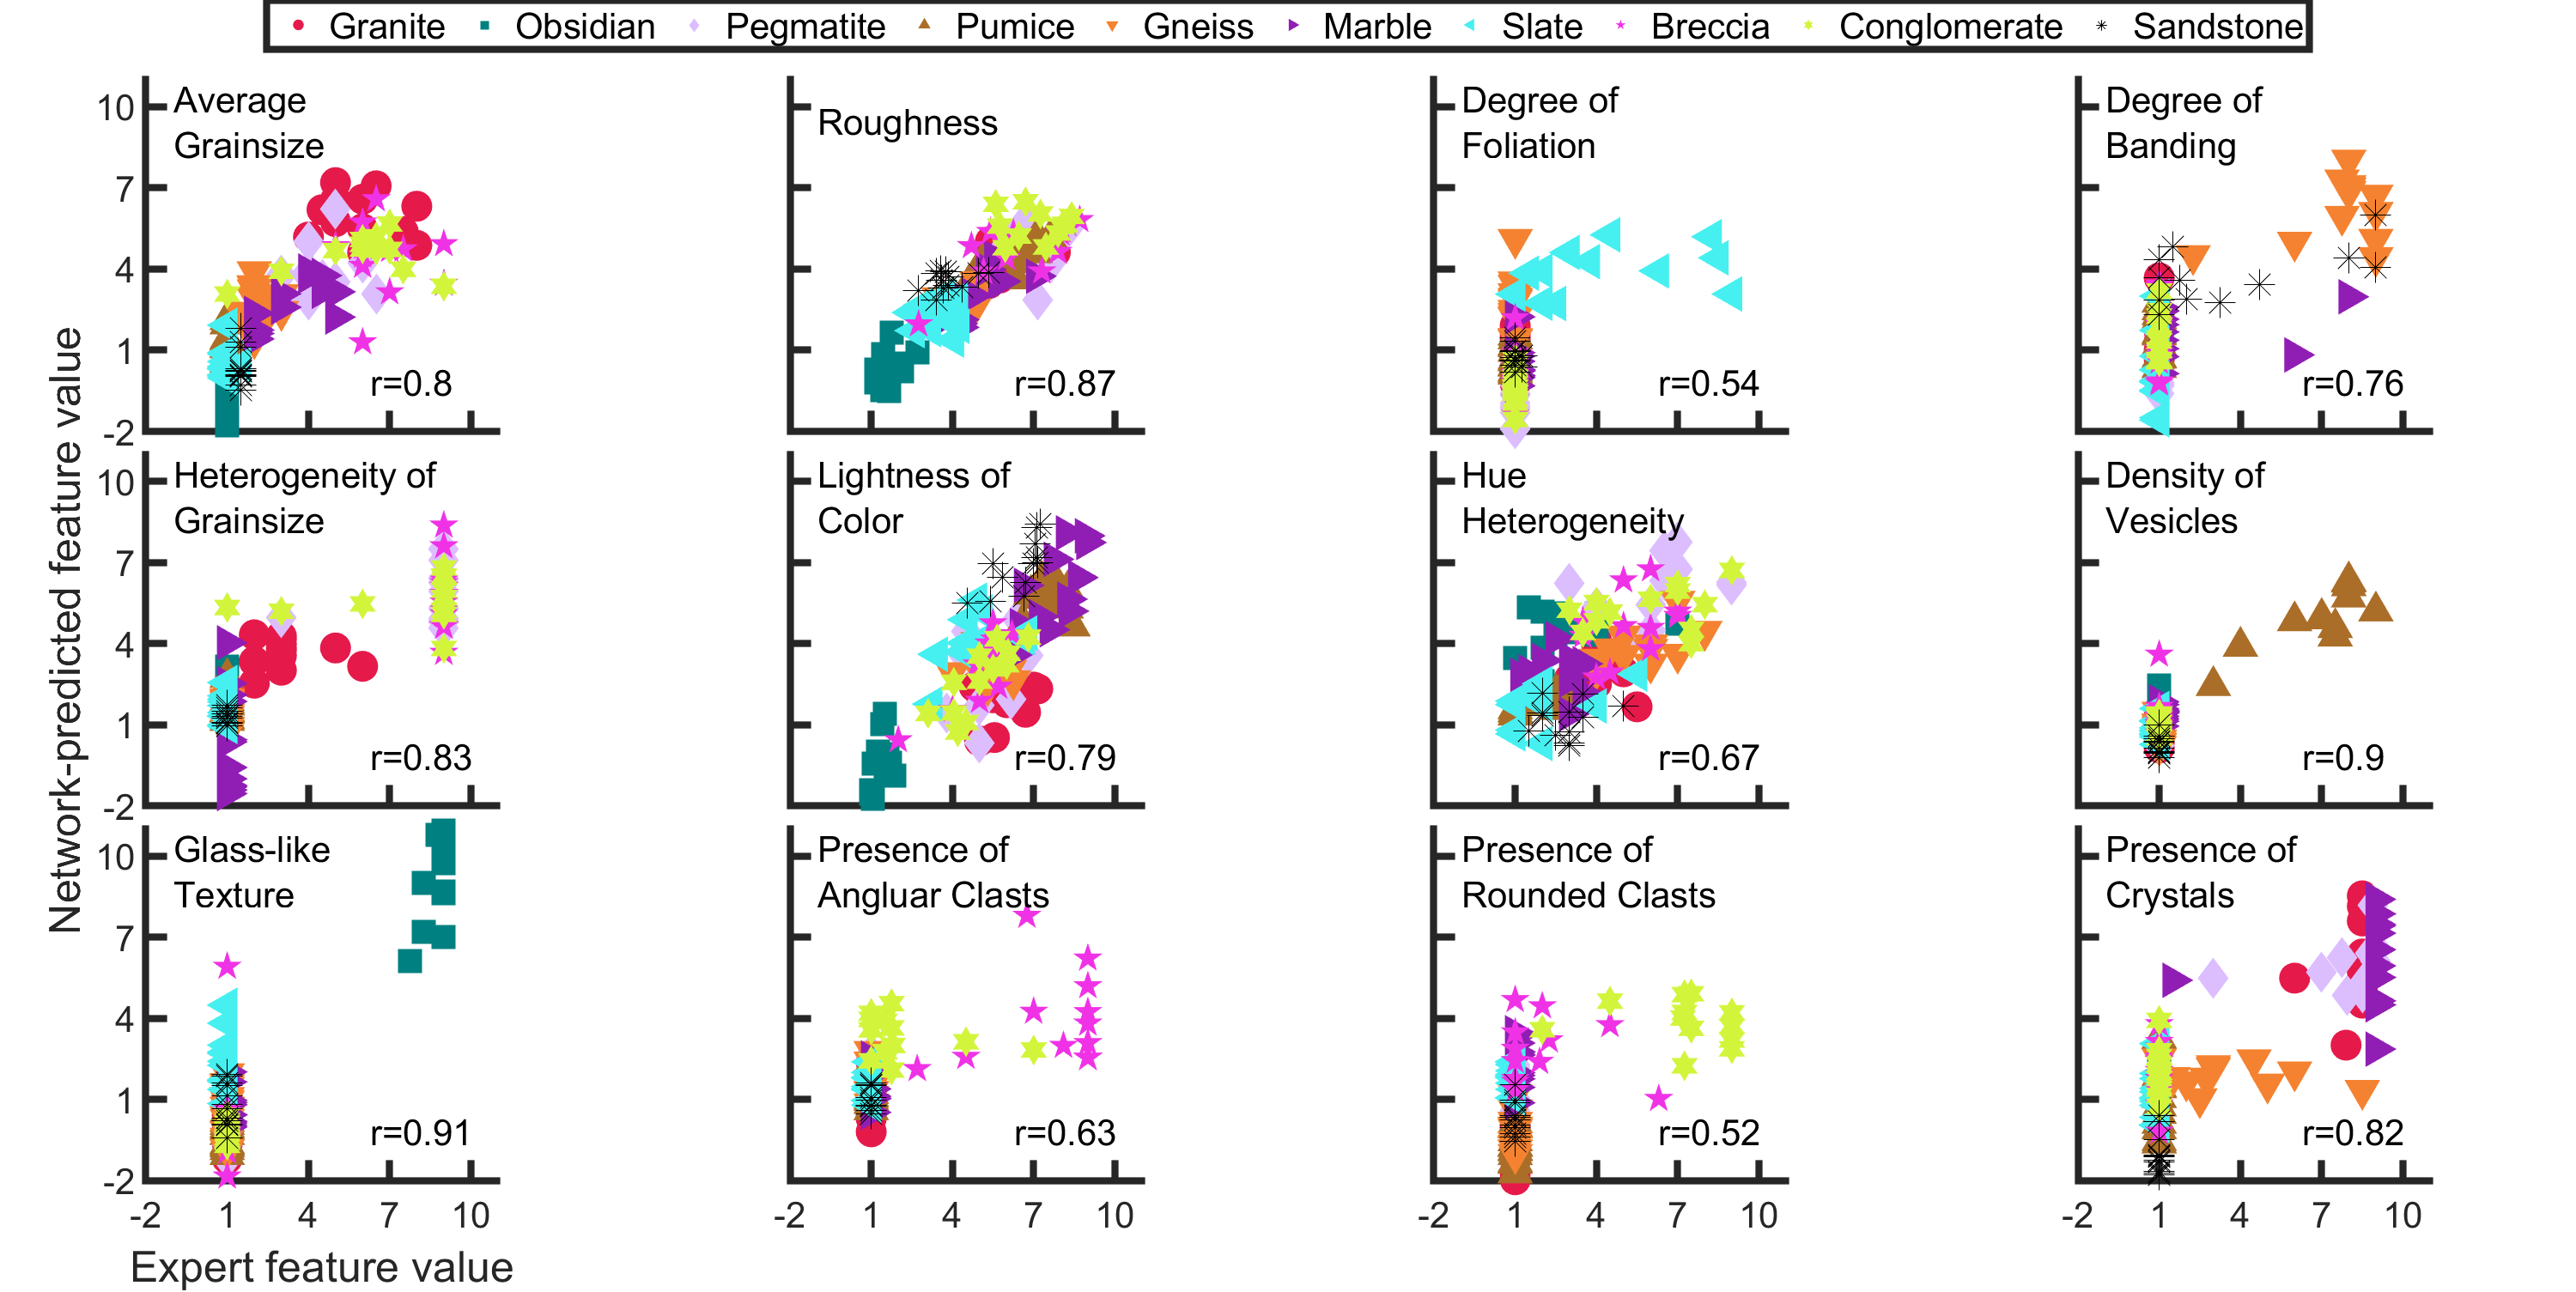
\includegraphics[width=\textwidth]{images/MATLAB Correlation - Hybrid_Vs_Expert - 12 Feautres - Continuous.png}
    \caption{Feature Correlation - Hybrid Sequential CBM Vs Expert Ratings - 12 Features - Continuous Crystal Rating} \label{fig:Feature Correlation - Hybrid Sequential CBM Vs Expert Ratings - 12 Features - Continuous Crystal Rating}
\end{figure}

\begin{figure}[H]
  \centering
    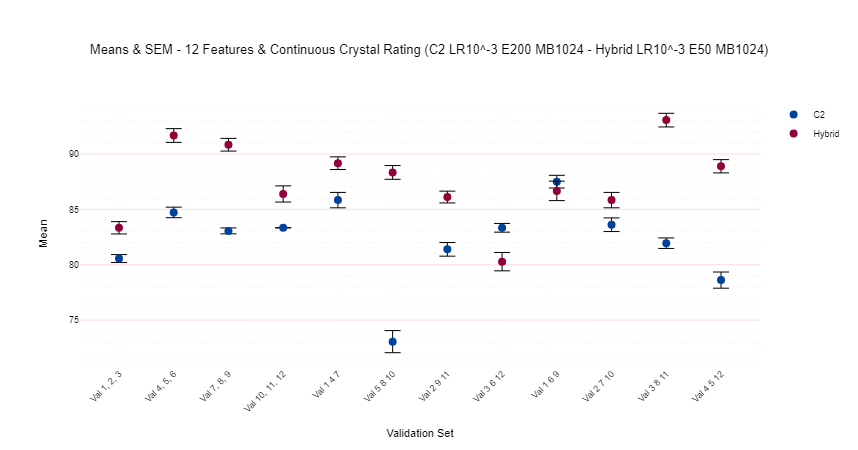
\includegraphics[width=\textwidth]{images/Means & SEM - 12 Features & Continuous Crystal Rating (C2 LR10^-3 E200 MB1024 - Hybrid LR10^-3 E50 MB1024).png}
    \caption{Means \& SEM - Validation Sets - 12 Features - Continuous Crystal Rating} \label{fig:Means & SEM - Validation Sets - 12 Features - Continuous Crystal Rating}
\end{figure}

\begin{figure}[H]
  \centering
    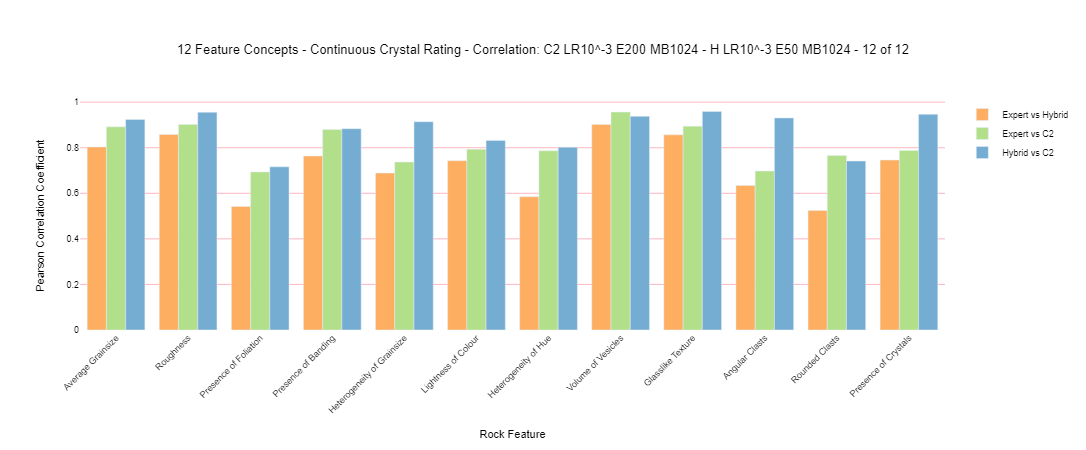
\includegraphics[width=\textwidth]{images/12 Feature Concepts - Continuous Crystal Rating - Correlation- C2 LR10^-3 E200 MB1024 - H LR10^-3 E50 MB1024 - 12 of 12.png}
    \caption{12 Feature Concepts - Continuous Crystal Rating - Mean correlation of Feature Concepts} \label{fig:12 Feature Concepts - Continuous Crystal Rating - Mean correlation of Feature Concepts}
\end{figure}


\begin{figure}[H]
  \centering
    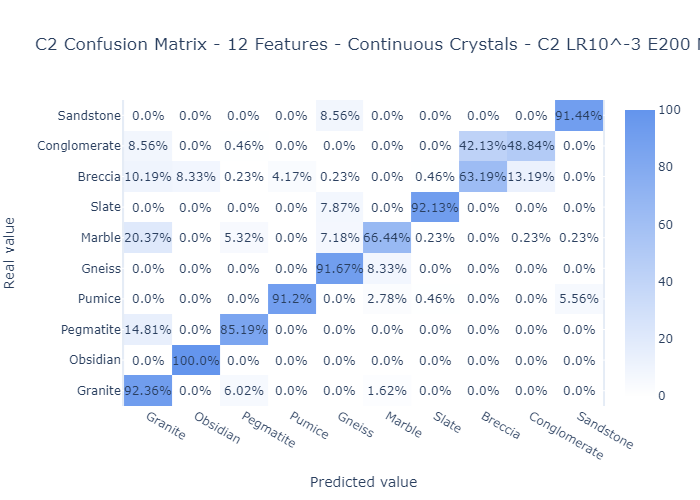
\includegraphics[width=\textwidth, trim = 0cm 0cm 0.5cm 3.5cm, clip]{images/C2 Confusion Matrix - 12 Features - Continuous Crystals.png}
    \caption{Sequential CBM Network Accuracy Confusion Matrix - 12 Features - Continuous Crystal Ratings} \label{fig:Sequential CBM Network Accuracy Confusion Matrix - 12 Features - Continuous Crystal Ratings}
\end{figure}

\begin{figure}[H]
  \centering
    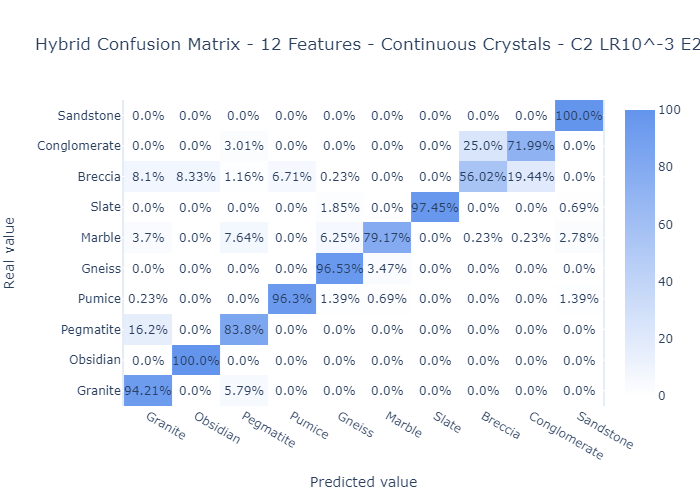
\includegraphics[width=0.9\textwidth, trim = 0cm 0cm 0.5cm 3.5cm, clip]{images/Hybrid Confusion Matrix - 12 Features - Continuous Crystals.png}
    \caption{Hybrid Network Accuracy Confusion Matrix - 12 Features - Continuous Crystal Ratings} \label{fig:Hybrid Network Accuracy Confusion Matrix- 12 Features - Continuous Crystal Ratings}
\end{figure}


\section{Tables}

\subsection{An Example of 13 Expert Feature Ratings for Granite Used for Training}
\scriptsize
\begin{longtable}[c]{@{}lllllllllllll@{}}
\toprule
%\addtolength{\tabcolsep}{-1pt}
\textbf{Rock   Type: Granite} &
   &
  \textbf{} &
  \textbf{} &
  \textbf{} &
  \textbf{} &
  \textbf{} &
  \textbf{} &
  \textbf{} &
  \textbf{} &
  \textbf{} &
  \textbf{} &
  \textbf{} \\
\endfirsthead
%
\multicolumn{13}{c}%
{{\bfseries Table \thetable\ continued from previous page}} \\
\endhead
%
 &
  \multicolumn{12}{c}{\textbf{Rock Image Instance}} \\
\multicolumn{1}{c}{\textbf{Feature}} &
  \cellcolor[HTML]{FFD966}\textbf{1} &
  \cellcolor[HTML]{FFD966}\textbf{2} &
  \cellcolor[HTML]{FFD966}\textbf{3} &
  \cellcolor[HTML]{FFD966}\textbf{4} &
  \cellcolor[HTML]{FFD966}\textbf{5} &
  \cellcolor[HTML]{FFD966}\textbf{6} &
  \cellcolor[HTML]{FFD966}\textbf{7} &
  \cellcolor[HTML]{FFD966}\textbf{8} &
  \cellcolor[HTML]{FFD966}\textbf{9} &
  \cellcolor[HTML]{FFD966}\textbf{10} &
  \cellcolor[HTML]{FFD966}\textbf{11} &
  \cellcolor[HTML]{FFD966}\textbf{12} \\
\cellcolor[HTML]{E2EFDA}\textbf{Average   Grainsize} &
  6.5 &
  4 &
  6 &
  4.5 &
  6 &
  5 &
  5 &
  5 &
  7.5 &
  6 &
  8 &
  8 \\
\cellcolor[HTML]{E2EFDA}\textbf{Roughness} &
  6.25 &
  5.3 &
  5.45 &
  5.35 &
  6.9 &
  5.15 &
  5.75 &
  5.05 &
  7.8 &
  6 &
  5.4 &
  5.65 \\
\cellcolor[HTML]{E2EFDA}\textbf{Presence of   Foliation} &
  1 &
  1 &
  1 &
  1 &
  1 &
  1 &
  1 &
  1 &
  1 &
  1 &
  1 &
  1 \\
\cellcolor[HTML]{E2EFDA}\textbf{Presence of   Banding} &
  1 &
  1 &
  1 &
  1 &
  1 &
  1 &
  1 &
  1 &
  1 &
  1 &
  1 &
  1 \\
\cellcolor[HTML]{E2EFDA}\textbf{Heterogeneity   of Grainsize} &
  3 &
  3 &
  6 &
  2 &
  3 &
  3 &
  2 &
  3 &
  5 &
  2 &
  3 &
  3 \\
\cellcolor[HTML]{E2EFDA}\textbf{Lightness of   Color} &
  5 &
  7.15 &
  6.25 &
  6 &
  5 &
  5.55 &
  6.45 &
  6.7 &
  4.8 &
  5.5 &
  7 &
  6.5 \\
\cellcolor[HTML]{E2EFDA}\textbf{Heterogeneity   of Hue} &
  5 &
  3 &
  4 &
  3.5 &
  4 &
  3.5 &
  3 &
  3 &
  4 &
  5.5 &
  4 &
  4 \\
\cellcolor[HTML]{E2EFDA}\textbf{Heterogeneity   of Brightness} &
  4 &
  5 &
  3 &
  5 &
  1.5 &
  2 &
  4 &
  3 &
  3 &
  2 &
  4 &
  2.5 \\
\cellcolor[HTML]{E2EFDA}\textbf{Volume of   Vesicles} &
  1 &
  1 &
  1 &
  1 &
  1 &
  1 &
  1 &
  1 &
  1 &
  1 &
  1 &
  1 \\
\cellcolor[HTML]{E2EFDA}\textbf{Glasslike   texture} &
  1 &
  1 &
  1 &
  1 &
  1 &
  1 &
  1 &
  1 &
  1 &
  1 &
  1 &
  1 \\
\cellcolor[HTML]{E2EFDA}\textbf{Angular Clasts} &
  1 &
  1 &
  1 &
  1 &
  1 &
  1 &
  1 &
  1 &
  1 &
  1 &
  1 &
  1 \\
\cellcolor[HTML]{E2EFDA}\textbf{Rounded Clasts} &
  1 &
  1 &
  1 &
  1 &
  1 &
  1 &
  1 &
  1 &
  1 &
  1 &
  1 &
  1 \\
\cellcolor[HTML]{E2EFDA}\textbf{Presence of   Crystals} &
  8.5 &
  8.5 &
  6 &
  8.5 &
  7.9 &
  8.5 &
  8.5 &
  8.5 &
  8.5 &
  8.5 &
  8.5 &
  8.5
\\
\caption{An Example of 13 Expert Feature Ratings for Granite - As Used for Training}
\label{An Example of 13 Expert Feature Ratings for Granite - As Used for Training}\\
\end{longtable}


\subsection{Feature Correlations - 13 Features - Continuous (Scalar) Crystal Rating 12 Runs of 12 Alternating Validation Sets}
\scriptsize
\begin{longtable}[c]{@{}llllllllll@{}}
\toprule
\addtolength{\tabcolsep}{-1pt}
\textbf{Set/Runs} &
  \cellcolor[HTML]{FCE4D6}\textbf{12/12} &
  \cellcolor[HTML]{FCE4D6}\textbf{12/12} &
  \cellcolor[HTML]{FCE4D6}\textbf{12/12} &
  \cellcolor[HTML]{FCE4D6}\textbf{12/12} &
  \cellcolor[HTML]{FCE4D6}\textbf{12/12} &
  \cellcolor[HTML]{FCE4D6}\textbf{12/12} &
  \cellcolor[HTML]{FCE4D6}\textbf{12/12} &
  \cellcolor[HTML]{FCE4D6}\textbf{12/12} &
  \cellcolor[HTML]{FCE4D6}\textbf{12/12} \\* \midrule
\endfirsthead
%
\multicolumn{10}{c}%
{{\bfseries Table \thetable\ continued from previous page}} \\
\endhead
%
\bottomrule
\endfoot
%
\endlastfoot
%
\rowcolor[HTML]{E7E6E6} 
\textbf{C2} &
   &
  \textbf{} &
  \textbf{} &
  \textbf{} &
  \textbf{} &
  \textbf{} &
  \textbf{} &
  \textbf{} &
  \textbf{} \\
\textbf{Epochs} &
  \cellcolor[HTML]{F8CBAD}\textbf{150} &
  \cellcolor[HTML]{C6E0B4}\textbf{200} &
  \cellcolor[HTML]{FFE699}\textbf{200} &
  \cellcolor[HTML]{B4C6E7}\textbf{400} &
  \cellcolor[HTML]{FCE4D6}\textbf{400} &
  \cellcolor[HTML]{E2EFDA}\textbf{400} &
  \cellcolor[HTML]{FFF2CC}\textbf{400} &
  \cellcolor[HTML]{DDEBF7}\textbf{400} &
  \cellcolor[HTML]{D6DCE4}\textbf{400} \\
\textbf{Learning Rate} &
  \cellcolor[HTML]{F8CBAD}{\color[HTML]{202124} \textbf{0.001}} &
  \cellcolor[HTML]{C6E0B4}{\color[HTML]{202124} \textbf{0.001}} &
  \cellcolor[HTML]{FFE699}{\color[HTML]{202124} \textbf{0.001}} &
  \cellcolor[HTML]{B4C6E7}{\color[HTML]{202124} \textbf{0.001}} &
  \cellcolor[HTML]{FCE4D6}{\color[HTML]{202124} \textbf{0.001}} &
  \cellcolor[HTML]{E2EFDA}{\color[HTML]{202124} \textbf{0.001}} &
  \cellcolor[HTML]{FFF2CC}{\color[HTML]{202124} \textbf{0.001}} &
  \cellcolor[HTML]{DDEBF7}{\color[HTML]{202124} \textbf{0.001}} &
  \cellcolor[HTML]{D6DCE4}{\color[HTML]{202124} \textbf{0.001}} \\
\textbf{Learning Rate} &
  \cellcolor[HTML]{F8CBAD}{\color[HTML]{202124} \textbf{10\textasciicircum{}-3}} &
  \cellcolor[HTML]{C6E0B4}{\color[HTML]{202124} \textbf{10\textasciicircum{}-3}} &
  \cellcolor[HTML]{FFE699}{\color[HTML]{202124} \textbf{10\textasciicircum{}-3}} &
  \cellcolor[HTML]{B4C6E7}{\color[HTML]{202124} \textbf{10\textasciicircum{}-3}} &
  \cellcolor[HTML]{FCE4D6}{\color[HTML]{202124} \textbf{10\textasciicircum{}-3}} &
  \cellcolor[HTML]{E2EFDA}{\color[HTML]{202124} \textbf{10\textasciicircum{}-3}} &
  \cellcolor[HTML]{FFF2CC}{\color[HTML]{202124} \textbf{10\textasciicircum{}-3}} &
  \cellcolor[HTML]{DDEBF7}{\color[HTML]{202124} \textbf{10\textasciicircum{}-3}} &
  \cellcolor[HTML]{D6DCE4}{\color[HTML]{202124} \textbf{10\textasciicircum{}-3}} \\
\textbf{Minibatch Size} &
  \cellcolor[HTML]{F8CBAD}{\color[HTML]{202124} \textbf{1024}} &
  \cellcolor[HTML]{C6E0B4}{\color[HTML]{202124} \textbf{1024}} &
  \cellcolor[HTML]{FFE699}{\color[HTML]{202124} \textbf{1024}} &
  \cellcolor[HTML]{B4C6E7}{\color[HTML]{202124} \textbf{1024}} &
  \cellcolor[HTML]{FCE4D6}{\color[HTML]{202124} \textbf{256}} &
  \cellcolor[HTML]{E2EFDA}{\color[HTML]{202124} \textbf{256}} &
  \cellcolor[HTML]{FFF2CC}{\color[HTML]{202124} \textbf{256}} &
  \cellcolor[HTML]{DDEBF7}{\color[HTML]{202124} \textbf{256}} &
  \cellcolor[HTML]{D6DCE4}{\color[HTML]{202124} \textbf{256}} \\
\cellcolor[HTML]{F2F2F2}\textbf{Correlation - Expert Feature   vs C2} &
  \cellcolor[HTML]{F8CBAD}\textbf{} &
  \cellcolor[HTML]{C6E0B4}\textbf{} &
  \cellcolor[HTML]{FFE699}\textbf{} &
  \cellcolor[HTML]{B4C6E7}\textbf{} &
  \cellcolor[HTML]{FCE4D6}{\color[HTML]{202124} \textbf{}} &
  \cellcolor[HTML]{E2EFDA}{\color[HTML]{202124} \textbf{}} &
  \cellcolor[HTML]{FFF2CC}{\color[HTML]{202124} \textbf{}} &
  \cellcolor[HTML]{DDEBF7}{\color[HTML]{202124} \textbf{}} &
  \cellcolor[HTML]{D6DCE4}{\color[HTML]{202124} \textbf{}} \\
\textbf{Average Grainsize} &
  \cellcolor[HTML]{F8CBAD}{\color[HTML]{202124} 0.89} &
  \cellcolor[HTML]{C6E0B4}0.89 &
  \cellcolor[HTML]{FFE699}0.89 &
  \cellcolor[HTML]{B4C6E7}0.89 &
  \cellcolor[HTML]{FCE4D6}{\color[HTML]{202124} 0.89} &
  \cellcolor[HTML]{E2EFDA}{\color[HTML]{202124} 0.89} &
  \cellcolor[HTML]{FFF2CC}{\color[HTML]{202124} 0.89} &
  \cellcolor[HTML]{DDEBF7}{\color[HTML]{202124} 0.89} &
  \cellcolor[HTML]{D6DCE4}{\color[HTML]{202124} 0.89} \\
\textbf{Roughness} &
  \cellcolor[HTML]{F8CBAD}{\color[HTML]{202124} 0.92} &
  \cellcolor[HTML]{C6E0B4}0.92 &
  \cellcolor[HTML]{FFE699}0.92 &
  \cellcolor[HTML]{B4C6E7}0.92 &
  \cellcolor[HTML]{FCE4D6}{\color[HTML]{202124} 0.92} &
  \cellcolor[HTML]{E2EFDA}{\color[HTML]{202124} 0.92} &
  \cellcolor[HTML]{FFF2CC}{\color[HTML]{202124} 0.92} &
  \cellcolor[HTML]{DDEBF7}{\color[HTML]{202124} 0.92} &
  \cellcolor[HTML]{D6DCE4}{\color[HTML]{202124} 0.92} \\
\textbf{Presence of Foliation} &
  \cellcolor[HTML]{F8CBAD}{\color[HTML]{202124} 0.67} &
  \cellcolor[HTML]{C6E0B4}0.67 &
  \cellcolor[HTML]{FFE699}0.67 &
  \cellcolor[HTML]{B4C6E7}0.67 &
  \cellcolor[HTML]{FCE4D6}{\color[HTML]{202124} 0.66} &
  \cellcolor[HTML]{E2EFDA}{\color[HTML]{202124} 0.67} &
  \cellcolor[HTML]{FFF2CC}{\color[HTML]{202124} 0.67} &
  \cellcolor[HTML]{DDEBF7}{\color[HTML]{202124} 0.67} &
  \cellcolor[HTML]{D6DCE4}{\color[HTML]{202124} 0.67} \\
\textbf{Presence of Banding} &
  \cellcolor[HTML]{F8CBAD}{\color[HTML]{202124} 0.88} &
  \cellcolor[HTML]{C6E0B4}0.88 &
  \cellcolor[HTML]{FFE699}0.88 &
  \cellcolor[HTML]{B4C6E7}0.88 &
  \cellcolor[HTML]{FCE4D6}{\color[HTML]{202124} 0.88} &
  \cellcolor[HTML]{E2EFDA}{\color[HTML]{202124} 0.88} &
  \cellcolor[HTML]{FFF2CC}{\color[HTML]{202124} 0.88} &
  \cellcolor[HTML]{DDEBF7}{\color[HTML]{202124} 0.88} &
  \cellcolor[HTML]{D6DCE4}{\color[HTML]{202124} 0.88} \\
\textbf{Heterogeneity of Grainsize} &
  \cellcolor[HTML]{F8CBAD}0.89 &
  \cellcolor[HTML]{C6E0B4}0.89 &
  \cellcolor[HTML]{FFE699}0.89 &
  \cellcolor[HTML]{B4C6E7}0.89 &
  \cellcolor[HTML]{FCE4D6}0.89 &
  \cellcolor[HTML]{E2EFDA}0.89 &
  \cellcolor[HTML]{FFF2CC}0.89 &
  \cellcolor[HTML]{DDEBF7}0.89 &
  \cellcolor[HTML]{D6DCE4}0.89 \\
\textbf{Lightness of Colour} &
  \cellcolor[HTML]{F8CBAD}0.93 &
  \cellcolor[HTML]{C6E0B4}0.93 &
  \cellcolor[HTML]{FFE699}0.93 &
  \cellcolor[HTML]{B4C6E7}0.93 &
  \cellcolor[HTML]{FCE4D6}0.93 &
  \cellcolor[HTML]{E2EFDA}0.93 &
  \cellcolor[HTML]{FFF2CC}0.93 &
  \cellcolor[HTML]{DDEBF7}0.93 &
  \cellcolor[HTML]{D6DCE4}0.93 \\
\textbf{Heterogeneity of Hue} &
  \cellcolor[HTML]{F8CBAD}0.84 &
  \cellcolor[HTML]{C6E0B4}0.84 &
  \cellcolor[HTML]{FFE699}0.84 &
  \cellcolor[HTML]{B4C6E7}0.84 &
  \cellcolor[HTML]{FCE4D6}0.84 &
  \cellcolor[HTML]{E2EFDA}0.84 &
  \cellcolor[HTML]{FFF2CC}0.84 &
  \cellcolor[HTML]{DDEBF7}0.84 &
  \cellcolor[HTML]{D6DCE4}0.84 \\
\textbf{Heterogeneity of Brightness} &
  \cellcolor[HTML]{F8CBAD}0.43 &
  \cellcolor[HTML]{C6E0B4}0.43 &
  \cellcolor[HTML]{FFE699}0.43 &
  \cellcolor[HTML]{B4C6E7}0.43 &
  \cellcolor[HTML]{FCE4D6}0.43 &
  \cellcolor[HTML]{E2EFDA}0.43 &
  \cellcolor[HTML]{FFF2CC}0.43 &
  \cellcolor[HTML]{DDEBF7}0.43 &
  \cellcolor[HTML]{D6DCE4}0.43 \\
\textbf{Volume of Vesicles} &
  \cellcolor[HTML]{F8CBAD}0.96 &
  \cellcolor[HTML]{C6E0B4}0.96 &
  \cellcolor[HTML]{FFE699}0.96 &
  \cellcolor[HTML]{B4C6E7}0.96 &
  \cellcolor[HTML]{FCE4D6}0.96 &
  \cellcolor[HTML]{E2EFDA}0.96 &
  \cellcolor[HTML]{FFF2CC}0.96 &
  \cellcolor[HTML]{DDEBF7}0.96 &
  \cellcolor[HTML]{D6DCE4}0.96 \\
\textbf{Glasslike Texture} &
  \cellcolor[HTML]{F8CBAD}0.95 &
  \cellcolor[HTML]{C6E0B4}0.95 &
  \cellcolor[HTML]{FFE699}0.95 &
  \cellcolor[HTML]{B4C6E7}0.95 &
  \cellcolor[HTML]{FCE4D6}0.95 &
  \cellcolor[HTML]{E2EFDA}0.95 &
  \cellcolor[HTML]{FFF2CC}0.95 &
  \cellcolor[HTML]{DDEBF7}0.95 &
  \cellcolor[HTML]{D6DCE4}0.95 \\
\textbf{Angular Clasts} &
  \cellcolor[HTML]{F8CBAD}0.70 &
  \cellcolor[HTML]{C6E0B4}0.70 &
  \cellcolor[HTML]{FFE699}0.70 &
  \cellcolor[HTML]{B4C6E7}0.70 &
  \cellcolor[HTML]{FCE4D6}0.70 &
  \cellcolor[HTML]{E2EFDA}0.70 &
  \cellcolor[HTML]{FFF2CC}0.70 &
  \cellcolor[HTML]{DDEBF7}0.70 &
  \cellcolor[HTML]{D6DCE4}0.70 \\
\textbf{Rounded Clasts} &
  \cellcolor[HTML]{F8CBAD}0.76 &
  \cellcolor[HTML]{C6E0B4}0.76 &
  \cellcolor[HTML]{FFE699}0.76 &
  \cellcolor[HTML]{B4C6E7}0.76 &
  \cellcolor[HTML]{FCE4D6}0.76 &
  \cellcolor[HTML]{E2EFDA}0.76 &
  \cellcolor[HTML]{FFF2CC}0.76 &
  \cellcolor[HTML]{DDEBF7}0.76 &
  \cellcolor[HTML]{D6DCE4}0.76 \\
\textbf{Presence of Crystals} &
  \cellcolor[HTML]{F8CBAD}0.88 &
  \cellcolor[HTML]{C6E0B4}0.88 &
  \cellcolor[HTML]{FFE699}0.88 &
  \cellcolor[HTML]{B4C6E7}0.88 &
  \cellcolor[HTML]{FCE4D6}0.88 &
  \cellcolor[HTML]{E2EFDA}0.88 &
  \cellcolor[HTML]{FFF2CC}0.88 &
  \cellcolor[HTML]{DDEBF7}0.88 &
  \cellcolor[HTML]{D6DCE4}0.88 \\
\cellcolor[HTML]{FFFF00}\textbf{Mean Correlation Ex Vs C2} &
  \textbf{0.8228} &
  \textbf{0.8230} &
  \textbf{0.8229} &
  \textbf{0.8222} &
  \textbf{0.8224} &
  \textbf{0.8232} &
  \textbf{0.8230} &
  \textbf{0.8222} &
  \textbf{0.8230} \\
\rowcolor[HTML]{E7E6E6} 
\textbf{Hybrid} &
   &
  \textbf{} &
  \textbf{} &
  \textbf{} &
  \textbf{} &
  \textbf{} &
  \textbf{} &
  \textbf{} &
  \textbf{} \\
\textbf{Epochs} &
  \cellcolor[HTML]{F8CBAD}\textbf{50} &
  \cellcolor[HTML]{C6E0B4}\textbf{200} &
  \cellcolor[HTML]{FFE699}\textbf{50} &
  \cellcolor[HTML]{B4C6E7}\textbf{50} &
  \cellcolor[HTML]{FCE4D6}\textbf{15} &
  \cellcolor[HTML]{E2EFDA}\textbf{25} &
  \cellcolor[HTML]{FFF2CC}\textbf{50} &
  \cellcolor[HTML]{DDEBF7}\textbf{100} &
  \cellcolor[HTML]{D6DCE4}\textbf{200} \\
\textbf{Learning Rate} &
  \cellcolor[HTML]{F8CBAD}{\color[HTML]{202124} \textbf{0.001}} &
  \cellcolor[HTML]{C6E0B4}{\color[HTML]{202124} \textbf{0.001}} &
  \cellcolor[HTML]{FFE699}{\color[HTML]{202124} \textbf{0.001}} &
  \cellcolor[HTML]{B4C6E7}{\color[HTML]{202124} \textbf{0.001}} &
  \cellcolor[HTML]{FCE4D6}{\color[HTML]{202124} \textbf{0.001}} &
  \cellcolor[HTML]{E2EFDA}{\color[HTML]{202124} \textbf{0.001}} &
  \cellcolor[HTML]{FFF2CC}{\color[HTML]{202124} \textbf{0.001}} &
  \cellcolor[HTML]{DDEBF7}{\color[HTML]{202124} \textbf{0.001}} &
  \cellcolor[HTML]{D6DCE4}{\color[HTML]{202124} \textbf{0.001}} \\
\textbf{Learning Rate} &
  \cellcolor[HTML]{F8CBAD}{\color[HTML]{202124} \textbf{10\textasciicircum{}-3}} &
  \cellcolor[HTML]{C6E0B4}{\color[HTML]{202124} \textbf{10\textasciicircum{}-3}} &
  \cellcolor[HTML]{FFE699}{\color[HTML]{202124} \textbf{10\textasciicircum{}-3}} &
  \cellcolor[HTML]{B4C6E7}{\color[HTML]{202124} \textbf{10\textasciicircum{}-3}} &
  \cellcolor[HTML]{FCE4D6}{\color[HTML]{202124} \textbf{10\textasciicircum{}-3}} &
  \cellcolor[HTML]{E2EFDA}{\color[HTML]{202124} \textbf{10\textasciicircum{}-3}} &
  \cellcolor[HTML]{FFF2CC}{\color[HTML]{202124} \textbf{10\textasciicircum{}-3}} &
  \cellcolor[HTML]{DDEBF7}{\color[HTML]{202124} \textbf{10\textasciicircum{}-3}} &
  \cellcolor[HTML]{D6DCE4}{\color[HTML]{202124} \textbf{10\textasciicircum{}-3}} \\
\textbf{Minibatch Size} &
  \cellcolor[HTML]{F8CBAD}\textbf{1024} &
  \cellcolor[HTML]{C6E0B4}{\color[HTML]{202124} \textbf{1024}} &
  \cellcolor[HTML]{FFE699}\textbf{1024} &
  \cellcolor[HTML]{B4C6E7}\textbf{1024} &
  \cellcolor[HTML]{FCE4D6}\textbf{1024} &
  \cellcolor[HTML]{E2EFDA}\textbf{1024} &
  \cellcolor[HTML]{FFF2CC}\textbf{1024} &
  \cellcolor[HTML]{DDEBF7}\textbf{1024} &
  \cellcolor[HTML]{D6DCE4}\textbf{1024} \\
\cellcolor[HTML]{F2F2F2}\textbf{Correlation - Expert Feature   vs Hybrid} &
  \cellcolor[HTML]{F8CBAD}{\color[HTML]{202124} \textbf{}} &
  \cellcolor[HTML]{C6E0B4}\textbf{} &
  \cellcolor[HTML]{FFE699}\textbf{} &
  \cellcolor[HTML]{B4C6E7}\textbf{} &
  \cellcolor[HTML]{FCE4D6}{\color[HTML]{202124} \textbf{}} &
  \cellcolor[HTML]{E2EFDA}{\color[HTML]{202124} \textbf{}} &
  \multicolumn{1}{c}{\cellcolor[HTML]{FFF2CC}{\color[HTML]{202124} \textbf{}}} &
  \cellcolor[HTML]{DDEBF7}{\color[HTML]{202124} \textbf{}} &
  \cellcolor[HTML]{D6DCE4}{\color[HTML]{202124} \textbf{}} \\
\textbf{Average Grainsize} &
  \cellcolor[HTML]{F8CBAD}{\color[HTML]{202124} 0.77} &
  \cellcolor[HTML]{C6E0B4}0.71 &
  \cellcolor[HTML]{FFE699}0.79 &
  \cellcolor[HTML]{B4C6E7}0.81 &
  \cellcolor[HTML]{FCE4D6}{\color[HTML]{202124} 0.84} &
  \cellcolor[HTML]{E2EFDA}{\color[HTML]{202124} 0.83} &
  \cellcolor[HTML]{FFF2CC}{\color[HTML]{202124} 0.81} &
  \cellcolor[HTML]{DDEBF7}{\color[HTML]{202124} 0.77} &
  \cellcolor[HTML]{D6DCE4}{\color[HTML]{202124} 0.67} \\
\textbf{Roughness} &
  \cellcolor[HTML]{F8CBAD}{\color[HTML]{202124} 0.87} &
  \cellcolor[HTML]{C6E0B4}0.76 &
  \cellcolor[HTML]{FFE699}0.86 &
  \cellcolor[HTML]{B4C6E7}0.86 &
  \cellcolor[HTML]{FCE4D6}{\color[HTML]{202124} 0.89} &
  \cellcolor[HTML]{E2EFDA}{\color[HTML]{202124} 0.88} &
  \cellcolor[HTML]{FFF2CC}{\color[HTML]{202124} 0.86} &
  \cellcolor[HTML]{DDEBF7}{\color[HTML]{202124} 0.81} &
  \cellcolor[HTML]{D6DCE4}{\color[HTML]{202124} 0.71} \\
\textbf{Presence of Foliation} &
  \cellcolor[HTML]{F8CBAD}{\color[HTML]{202124} 0.52} &
  \cellcolor[HTML]{C6E0B4}0.59 &
  \cellcolor[HTML]{FFE699}0.55 &
  \cellcolor[HTML]{B4C6E7}0.59 &
  \cellcolor[HTML]{FCE4D6}{\color[HTML]{202124} 0.60} &
  \cellcolor[HTML]{E2EFDA}{\color[HTML]{202124} 0.61} &
  \cellcolor[HTML]{FFF2CC}{\color[HTML]{202124} 0.60} &
  \cellcolor[HTML]{DDEBF7}{\color[HTML]{202124} 0.60} &
  \cellcolor[HTML]{D6DCE4}{\color[HTML]{202124} 0.65} \\
\textbf{Presence of Banding} &
  \cellcolor[HTML]{F8CBAD}0.74 &
  \cellcolor[HTML]{C6E0B4}0.73 &
  \cellcolor[HTML]{FFE699}0.76 &
  \cellcolor[HTML]{B4C6E7}0.80 &
  \cellcolor[HTML]{FCE4D6}0.83 &
  \cellcolor[HTML]{E2EFDA}0.83 &
  \cellcolor[HTML]{FFF2CC}0.81 &
  \cellcolor[HTML]{DDEBF7}0.79 &
  \cellcolor[HTML]{D6DCE4}0.72 \\
\textbf{Heterogeneity of Grainsize} &
  \cellcolor[HTML]{F8CBAD}0.85 &
  \cellcolor[HTML]{C6E0B4}0.82 &
  \cellcolor[HTML]{FFE699}0.85 &
  \cellcolor[HTML]{B4C6E7}0.86 &
  \cellcolor[HTML]{FCE4D6}0.88 &
  \cellcolor[HTML]{E2EFDA}0.87 &
  \cellcolor[HTML]{FFF2CC}0.86 &
  \cellcolor[HTML]{DDEBF7}0.84 &
  \cellcolor[HTML]{D6DCE4}0.82 \\
\textbf{Lightness of Colour} &
  \cellcolor[HTML]{F8CBAD}0.75 &
  \cellcolor[HTML]{C6E0B4}0.49 &
  \cellcolor[HTML]{FFE699}0.76 &
  \cellcolor[HTML]{B4C6E7}0.78 &
  \cellcolor[HTML]{FCE4D6}0.85 &
  \cellcolor[HTML]{E2EFDA}0.83 &
  \cellcolor[HTML]{FFF2CC}0.80 &
  \cellcolor[HTML]{DDEBF7}0.70 &
  \cellcolor[HTML]{D6DCE4}0.57 \\
\textbf{Heterogeneity of Hue} &
  \cellcolor[HTML]{F8CBAD}0.71 &
  \cellcolor[HTML]{C6E0B4}0.67 &
  \cellcolor[HTML]{FFE699}0.69 &
  \cellcolor[HTML]{B4C6E7}0.67 &
  \cellcolor[HTML]{FCE4D6}0.74 &
  \cellcolor[HTML]{E2EFDA}0.72 &
  \cellcolor[HTML]{FFF2CC}0.67 &
  \cellcolor[HTML]{DDEBF7}0.61 &
  \cellcolor[HTML]{D6DCE4}0.57 \\
\textbf{Heterogeneity of Brightness} &
  \cellcolor[HTML]{F8CBAD}0.27 &
  \cellcolor[HTML]{C6E0B4}0.22 &
  \cellcolor[HTML]{FFE699}0.30 &
  \cellcolor[HTML]{B4C6E7}0.32 &
  \cellcolor[HTML]{FCE4D6}0.36 &
  \cellcolor[HTML]{E2EFDA}0.34 &
  \cellcolor[HTML]{FFF2CC}0.32 &
  \cellcolor[HTML]{DDEBF7}0.28 &
  \cellcolor[HTML]{D6DCE4}0.21 \\
\textbf{Volume of Vesicles} &
  \cellcolor[HTML]{F8CBAD}0.70 &
  \cellcolor[HTML]{C6E0B4}0.81 &
  \cellcolor[HTML]{FFE699}0.76 &
  \cellcolor[HTML]{B4C6E7}0.90 &
  \cellcolor[HTML]{FCE4D6}0.93 &
  \cellcolor[HTML]{E2EFDA}0.93 &
  \cellcolor[HTML]{FFF2CC}0.90 &
  \cellcolor[HTML]{DDEBF7}0.88 &
  \cellcolor[HTML]{D6DCE4}0.85 \\
\textbf{Glasslike Texture} &
  \cellcolor[HTML]{F8CBAD}0.92 &
  \cellcolor[HTML]{C6E0B4}0.93 &
  \cellcolor[HTML]{FFE699}0.93 &
  \cellcolor[HTML]{B4C6E7}0.94 &
  \cellcolor[HTML]{FCE4D6}0.95 &
  \cellcolor[HTML]{E2EFDA}0.95 &
  \cellcolor[HTML]{FFF2CC}0.94 &
  \cellcolor[HTML]{DDEBF7}0.94 &
  \cellcolor[HTML]{D6DCE4}0.93 \\
\textbf{Angular Clasts} &
  \cellcolor[HTML]{F8CBAD}0.58 &
  \cellcolor[HTML]{C6E0B4}0.53 &
  \cellcolor[HTML]{FFE699}0.60 &
  \cellcolor[HTML]{B4C6E7}0.62 &
  \cellcolor[HTML]{FCE4D6}0.64 &
  \cellcolor[HTML]{E2EFDA}0.63 &
  \cellcolor[HTML]{FFF2CC}0.61 &
  \cellcolor[HTML]{DDEBF7}0.57 &
  \cellcolor[HTML]{D6DCE4}0.53 \\
\textbf{Rounded Clasts} &
  \cellcolor[HTML]{F8CBAD}0.52 &
  \cellcolor[HTML]{C6E0B4}0.44 &
  \cellcolor[HTML]{FFE699}0.55 &
  \cellcolor[HTML]{B4C6E7}0.61 &
  \cellcolor[HTML]{FCE4D6}0.65 &
  \cellcolor[HTML]{E2EFDA}0.65 &
  \cellcolor[HTML]{FFF2CC}0.64 &
  \cellcolor[HTML]{DDEBF7}0.61 &
  \cellcolor[HTML]{D6DCE4}0.56 \\
\textbf{Presence of Crystals} &
  \cellcolor[HTML]{F8CBAD}0.83 &
  \cellcolor[HTML]{C6E0B4}0.71 &
  \cellcolor[HTML]{FFE699}0.84 &
  \cellcolor[HTML]{B4C6E7}0.85 &
  \cellcolor[HTML]{FCE4D6}0.86 &
  \cellcolor[HTML]{E2EFDA}0.86 &
  \cellcolor[HTML]{FFF2CC}0.85 &
  \cellcolor[HTML]{DDEBF7}0.82 &
  \cellcolor[HTML]{D6DCE4}0.77 \\
\cellcolor[HTML]{FFFF00}\textbf{Mean Correlation Ex Vs Hybrid} &
  \textbf{0.6944} &
  \textbf{0.6468} &
  \textbf{0.7116} &
  \cellcolor[HTML]{FFD966}\textbf{0.7385} &
  \cellcolor[HTML]{FFFF00}\textbf{0.7711} &
  \cellcolor[HTML]{FFD966}\textbf{0.7631} &
  \cellcolor[HTML]{FFD966}\textbf{0.7442} &
  \textbf{0.7084} &
  \textbf{0.6584} \\
\rowcolor[HTML]{E7E6E6} 
\textbf{Correlation -   Hybrid vs C2} &
   &
  \textbf{} &
  \textbf{} &
  \textbf{} &
  \textbf{} &
  \textbf{} &
  \textbf{} &
  \textbf{} &
  \textbf{} \\
\textbf{Average   Grainsize} &
  \cellcolor[HTML]{F8CBAD}{\color[HTML]{202124} 0.89} &
  \cellcolor[HTML]{C6E0B4}0.83 &
  \cellcolor[HTML]{FFE699}0.91 &
  \cellcolor[HTML]{B4C6E7}0.93 &
  \cellcolor[HTML]{FCE4D6}{\color[HTML]{202124} 0.96} &
  \cellcolor[HTML]{E2EFDA}{\color[HTML]{202124} 0.95} &
  \cellcolor[HTML]{FFF2CC}{\color[HTML]{202124} 0.93} &
  \cellcolor[HTML]{DDEBF7}{\color[HTML]{202124} 0.89} &
  \cellcolor[HTML]{D6DCE4}{\color[HTML]{202124} 0.80} \\
\textbf{Roughness} &
  \cellcolor[HTML]{F8CBAD}{\color[HTML]{202124} 0.94} &
  \cellcolor[HTML]{C6E0B4}0.83 &
  \cellcolor[HTML]{FFE699}0.94 &
  \cellcolor[HTML]{B4C6E7}0.95 &
  \cellcolor[HTML]{FCE4D6}{\color[HTML]{202124} 0.98} &
  \cellcolor[HTML]{E2EFDA}{\color[HTML]{202124} 0.97} &
  \cellcolor[HTML]{FFF2CC}{\color[HTML]{202124} 0.95} &
  \cellcolor[HTML]{DDEBF7}{\color[HTML]{202124} 0.90} &
  \cellcolor[HTML]{D6DCE4}{\color[HTML]{202124} 0.81} \\
\textbf{Presence of Foliation} &
  \cellcolor[HTML]{F8CBAD}{\color[HTML]{202124} 0.72} &
  \cellcolor[HTML]{C6E0B4}0.73 &
  \cellcolor[HTML]{FFE699}0.76 &
  \cellcolor[HTML]{B4C6E7}0.84 &
  \cellcolor[HTML]{FCE4D6}{\color[HTML]{202124} 0.88} &
  \cellcolor[HTML]{E2EFDA}{\color[HTML]{202124} 0.87} &
  \cellcolor[HTML]{FFF2CC}{\color[HTML]{202124} 0.85} &
  \cellcolor[HTML]{DDEBF7}{\color[HTML]{202124} 0.82} &
  \cellcolor[HTML]{D6DCE4}{\color[HTML]{202124} 0.85} \\
\textbf{Presence of Banding} &
  \cellcolor[HTML]{F8CBAD}0.85 &
  \cellcolor[HTML]{C6E0B4}0.83 &
  \cellcolor[HTML]{FFE699}0.89 &
  \cellcolor[HTML]{B4C6E7}0.94 &
  \cellcolor[HTML]{FCE4D6}0.97 &
  \cellcolor[HTML]{E2EFDA}0.96 &
  \cellcolor[HTML]{FFF2CC}0.95 &
  \cellcolor[HTML]{DDEBF7}0.91 &
  \cellcolor[HTML]{D6DCE4}0.82 \\
\textbf{Heterogeneity of Grainsize} &
  \cellcolor[HTML]{F8CBAD}0.94 &
  \cellcolor[HTML]{C6E0B4}0.89 &
  \cellcolor[HTML]{FFE699}0.94 &
  \cellcolor[HTML]{B4C6E7}0.95 &
  \cellcolor[HTML]{FCE4D6}0.98 &
  \cellcolor[HTML]{E2EFDA}0.97 &
  \cellcolor[HTML]{FFF2CC}0.95 &
  \cellcolor[HTML]{DDEBF7}0.93 &
  \cellcolor[HTML]{D6DCE4}0.90 \\
\textbf{Lightness of Colour} &
  \cellcolor[HTML]{F8CBAD}0.79 &
  \cellcolor[HTML]{C6E0B4}0.52 &
  \cellcolor[HTML]{FFE699}0.81 &
  \cellcolor[HTML]{B4C6E7}0.84 &
  \cellcolor[HTML]{FCE4D6}0.92 &
  \cellcolor[HTML]{E2EFDA}0.91 &
  \cellcolor[HTML]{FFF2CC}0.87 &
  \cellcolor[HTML]{DDEBF7}0.76 &
  \cellcolor[HTML]{D6DCE4}0.61 \\
\textbf{Heterogeneity of Hue} &
  \cellcolor[HTML]{F8CBAD}0.83 &
  \cellcolor[HTML]{C6E0B4}0.76 &
  \cellcolor[HTML]{FFE699}0.81 &
  \cellcolor[HTML]{B4C6E7}0.80 &
  \cellcolor[HTML]{FCE4D6}0.89 &
  \cellcolor[HTML]{E2EFDA}0.86 &
  \cellcolor[HTML]{FFF2CC}0.80 &
  \cellcolor[HTML]{DDEBF7}0.72 &
  \cellcolor[HTML]{D6DCE4}0.67 \\
\textbf{Heterogeneity of Brightness} &
  \cellcolor[HTML]{F8CBAD}0.60 &
  \cellcolor[HTML]{C6E0B4}0.42 &
  \cellcolor[HTML]{FFE699}0.68 &
  \cellcolor[HTML]{B4C6E7}0.77 &
  \cellcolor[HTML]{FCE4D6}0.85 &
  \cellcolor[HTML]{E2EFDA}0.80 &
  \cellcolor[HTML]{FFF2CC}0.73 &
  \cellcolor[HTML]{DDEBF7}0.61 &
  \cellcolor[HTML]{D6DCE4}0.39 \\
\textbf{Volume of Vesicles} &
  \cellcolor[HTML]{F8CBAD}0.71 &
  \cellcolor[HTML]{C6E0B4}0.83 &
  \cellcolor[HTML]{FFE699}0.77 &
  \cellcolor[HTML]{B4C6E7}0.92 &
  \cellcolor[HTML]{FCE4D6}0.96 &
  \cellcolor[HTML]{E2EFDA}0.95 &
  \cellcolor[HTML]{FFF2CC}0.92 &
  \cellcolor[HTML]{DDEBF7}0.89 &
  \cellcolor[HTML]{D6DCE4}0.87 \\
\textbf{Glasslike Texture} &
  \cellcolor[HTML]{F8CBAD}0.97 &
  \cellcolor[HTML]{C6E0B4}0.97 &
  \cellcolor[HTML]{FFE699}0.98 &
  \cellcolor[HTML]{B4C6E7}0.98 &
  \cellcolor[HTML]{FCE4D6}0.99 &
  \cellcolor[HTML]{E2EFDA}0.99 &
  \cellcolor[HTML]{FFF2CC}0.99 &
  \cellcolor[HTML]{DDEBF7}0.98 &
  \cellcolor[HTML]{D6DCE4}0.98 \\
\textbf{Angular Clasts} &
  \cellcolor[HTML]{F8CBAD}0.82 &
  \cellcolor[HTML]{C6E0B4}0.82 &
  \cellcolor[HTML]{FFE699}0.87 &
  \cellcolor[HTML]{B4C6E7}0.91 &
  \cellcolor[HTML]{FCE4D6}0.94 &
  \cellcolor[HTML]{E2EFDA}0.93 &
  \cellcolor[HTML]{FFF2CC}0.91 &
  \cellcolor[HTML]{DDEBF7}0.88 &
  \cellcolor[HTML]{D6DCE4}0.84 \\
\textbf{Rounded Clasts} &
  \cellcolor[HTML]{F8CBAD}0.73 &
  \cellcolor[HTML]{C6E0B4}0.61 &
  \cellcolor[HTML]{FFE699}0.78 &
  \cellcolor[HTML]{B4C6E7}0.85 &
  \cellcolor[HTML]{FCE4D6}0.92 &
  \cellcolor[HTML]{E2EFDA}0.91 &
  \cellcolor[HTML]{FFF2CC}0.89 &
  \cellcolor[HTML]{DDEBF7}0.84 &
  \cellcolor[HTML]{D6DCE4}0.79 \\
\textbf{Presence of Crystals} &
  \cellcolor[HTML]{F8CBAD}0.94 &
  \cellcolor[HTML]{C6E0B4}0.76 &
  \cellcolor[HTML]{FFE699}0.94 &
  \cellcolor[HTML]{B4C6E7}0.95 &
  \cellcolor[HTML]{FCE4D6}0.98 &
  \cellcolor[HTML]{E2EFDA}0.97 &
  \cellcolor[HTML]{FFF2CC}0.95 &
  \cellcolor[HTML]{DDEBF7}0.90 &
  \cellcolor[HTML]{D6DCE4}0.83 \\
\cellcolor[HTML]{FFFF00}\textbf{Mean   Correlation Hybrid Vs C2} &
  \textbf{0.8264} &
  \textbf{0.7534} &
  \textbf{0.8535} &
  \cellcolor[HTML]{FFD966}\textbf{0.8947} &
  \cellcolor[HTML]{FFFF00}\textbf{0.9388} &
  \cellcolor[HTML]{FFD966}\textbf{0.9256} &
  \cellcolor[HTML]{FFD966}\textbf{0.8985} &
  \textbf{0.8501} &
  \textbf{0.7801} \\* \bottomrule
  \\
\caption{Feature Correlations - 13 Features - Continuous (Scalar) Crystal Rating 12 Runs of 12 Alternating Validation Sets}
\label{Feature Correlations - 13 Features - Continuous (Scalar) Crystal Rating 12 Runs of 12 Alternating Validation Sets}\\
\end{longtable}

\subsection{Feature Correlations - 13 Features - Continuous (Scalar) Crystal Rating 1 Run of 12 Alternating Validation Sets}
\setcounter{table}{0}
\renewcommand\thetable{\arabic{chapter}.\arabic{section}.\arabic{table}}
%\counterwithin{table}{subsection}
\scriptsize
\begin{longtable}[c]{@{}llllllllll@{}}
\toprule
\addtolength{\tabcolsep}{-1pt}
\textbf{Set/Runs} &
  1/12 &
  1/12 &
  1/12 &
  1/12 &
  1/12 &
  1/12 &
  1/12 &
  1/12 &
  1/12 \\
\endfirsthead
%
\multicolumn{10}{c}%
{{\bfseries Table \thetable\ continued from previous page}} \\
\endhead
%
\rowcolor[HTML]{E7E6E6} 
\textbf{C2} &
  \textbf{} &
  \textbf{} &
  \textbf{} &
  \textbf{} &
  \textbf{} &
  \textbf{} &
  \textbf{} &
  \textbf{} &
  \textbf{} \\
\textbf{Epochs} &
  \cellcolor[HTML]{FFF2CC}\textbf{150} &
  \cellcolor[HTML]{FCE4D6}\textbf{200} &
  \cellcolor[HTML]{FCE4D6}\textbf{200} &
  \cellcolor[HTML]{FCE4D6}\textbf{200} &
  \cellcolor[HTML]{FCE4D6}\textbf{200} &
  \cellcolor[HTML]{FCE4D6}\textbf{200} &
  \cellcolor[HTML]{FCE4D6}\textbf{200} &
  \cellcolor[HTML]{FCE4D6}\textbf{200} &
  \cellcolor[HTML]{FFF2CC}\textbf{100} \\
\textbf{Learning Rate} &
  \cellcolor[HTML]{FCE4D6}\textbf{0.001} &
  \cellcolor[HTML]{FCE4D6}{\color[HTML]{202124} \textbf{0.001}} &
  \cellcolor[HTML]{FCE4D6}{\color[HTML]{202124} \textbf{0.001}} &
  \cellcolor[HTML]{FCE4D6}{\color[HTML]{202124} \textbf{0.001}} &
  \cellcolor[HTML]{FCE4D6}{\color[HTML]{202124} \textbf{0.001}} &
  \cellcolor[HTML]{FCE4D6}{\color[HTML]{202124} \textbf{0.001}} &
  \cellcolor[HTML]{FCE4D6}{\color[HTML]{202124} \textbf{0.001}} &
  \cellcolor[HTML]{FCE4D6}{\color[HTML]{202124} \textbf{0.001}} &
  \cellcolor[HTML]{FFF2CC}\textbf{0.01} \\
\textbf{Learning Rate} &
  \cellcolor[HTML]{FCE4D6}\textbf{10\textasciicircum{}-3} &
  \cellcolor[HTML]{FCE4D6}\textbf{10\textasciicircum{}-3} &
  \cellcolor[HTML]{FCE4D6}\textbf{10\textasciicircum{}-3} &
  \cellcolor[HTML]{FCE4D6}\textbf{10\textasciicircum{}-3} &
  \cellcolor[HTML]{FCE4D6}\textbf{10\textasciicircum{}-3} &
  \cellcolor[HTML]{FCE4D6}\textbf{10\textasciicircum{}-3} &
  \cellcolor[HTML]{FCE4D6}\textbf{10\textasciicircum{}-3} &
  \cellcolor[HTML]{FCE4D6}\textbf{10\textasciicircum{}-3} &
  \cellcolor[HTML]{FCE4D6}\textbf{10\textasciicircum{}-3} \\
\textbf{Minibatch Size} &
  \cellcolor[HTML]{FCE4D6}\textbf{1024} &
  \cellcolor[HTML]{FCE4D6}\textbf{1024} &
  \cellcolor[HTML]{FCE4D6}\textbf{1024} &
  \cellcolor[HTML]{FCE4D6}\textbf{1024} &
  \cellcolor[HTML]{FCE4D6}\textbf{1024} &
  \cellcolor[HTML]{FCE4D6}\textbf{1024} &
  \cellcolor[HTML]{FCE4D6}\textbf{1024} &
  \cellcolor[HTML]{FCE4D6}\textbf{1024} &
  \cellcolor[HTML]{FCE4D6}\textbf{1024} \\
\rowcolor[HTML]{F2F2F2} 
\textbf{Correlation - Expert Feature   vs C2} &
  \textbf{} &
  \textbf{} &
  \textbf{} &
  \textbf{} &
  \textbf{} &
  \textbf{} &
  \textbf{} &
  \textbf{} &
  \textbf{} \\
\textbf{Average Grainsize} &
  0.89 &
  0.89 &
  0.89 &
  0.89 &
  0.89 &
  0.89 &
  0.89 &
  0.89 &
  0.89 \\
\textbf{Roughness} &
  0.92 &
  0.92 &
  0.92 &
  0.92 &
  0.92 &
  0.92 &
  0.92 &
  0.92 &
  0.92 \\
\textbf{Presence of Foliation} &
  0.66 &
  0.67 &
  0.68 &
  0.66 &
  0.67 &
  0.67 &
  0.67 &
  0.67 &
  0.67 \\
\textbf{Presence of Banding} &
  0.87 &
  0.88 &
  0.87 &
  0.88 &
  0.87 &
  0.87 &
  0.87 &
  0.88 &
  0.88 \\
\textbf{Heterogeneity of Grainsize} &
  0.89 &
  0.89 &
  0.89 &
  0.89 &
  0.88 &
  0.88 &
  0.89 &
  0.89 &
  0.89 \\
\textbf{Lightness of Colour} &
  0.93 &
  0.93 &
  0.92 &
  0.93 &
  0.93 &
  0.93 &
  0.93 &
  0.93 &
  0.93 \\
\textbf{Heterogeneity of Hue} &
  0.83 &
  0.83 &
  0.83 &
  0.84 &
  0.83 &
  0.83 &
  0.84 &
  0.83 &
  0.83 \\
\textbf{Heterogeneity of Brightness} &
  0.44 &
  0.43 &
  0.43 &
  0.43 &
  0.43 &
  0.43 &
  0.43 &
  0.43 &
  0.43 \\
\textbf{Volume of Vesicles} &
  0.96 &
  0.96 &
  0.97 &
  0.96 &
  0.96 &
  0.96 &
  0.96 &
  0.96 &
  0.96 \\
\textbf{Glasslike Texture} &
  0.95 &
  0.95 &
  0.95 &
  0.95 &
  0.95 &
  0.95 &
  0.95 &
  0.95 &
  0.95 \\
\textbf{Angular Clasts} &
  0.70 &
  0.70 &
  0.70 &
  0.70 &
  0.69 &
  0.69 &
  0.70 &
  0.70 &
  0.70 \\
\textbf{Rounded Clasts} &
  0.76 &
  0.76 &
  0.76 &
  0.76 &
  0.76 &
  0.76 &
  0.76 &
  0.76 &
  0.76 \\
\textbf{Presence of Crystals} &
  0.88 &
  0.88 &
  0.88 &
  0.88 &
  0.88 &
  0.88 &
  0.88 &
  0.88 &
  0.88 \\
\cellcolor[HTML]{FFFF00}\textbf{Mean Correlation Ex Vs C2} &
  \textbf{0.8220} &
  \textbf{0.8228} &
  \textbf{0.8223} &
  \textbf{0.8213} &
  \textbf{0.8203} &
  \textbf{0.8203} &
  \textbf{0.8221} &
  \textbf{0.8231} &
  \textbf{0.8228} \\
\rowcolor[HTML]{E7E6E6} 
\textbf{Hybrid} &
  \textbf{} &
  \textbf{} &
  \textbf{} &
  \textbf{} &
  \textbf{} &
  \textbf{} &
  \textbf{} &
  \textbf{} &
  \textbf{} \\
\textbf{Epochs} &
  \cellcolor[HTML]{FFF2CC}\textbf{150} &
  \cellcolor[HTML]{FFF2CC}\textbf{200} &
  \cellcolor[HTML]{FFF2CC}\textbf{300} &
  \cellcolor[HTML]{FFF2CC}\textbf{400} &
  \cellcolor[HTML]{FCE4D6}\textbf{200} &
  \cellcolor[HTML]{FCE4D6}\textbf{200} &
  \cellcolor[HTML]{FCE4D6}\textbf{200} &
  \cellcolor[HTML]{FCE4D6}\textbf{200} &
  \cellcolor[HTML]{FCE4D6}\textbf{200} \\
\textbf{Learning Rate} &
  \cellcolor[HTML]{FFF2CC}{\color[HTML]{202124} \textbf{0.001}} &
  \cellcolor[HTML]{FFF2CC}{\color[HTML]{202124} \textbf{0.0009}} &
  \cellcolor[HTML]{FFF2CC}{\color[HTML]{202124} \textbf{0.0007}} &
  \cellcolor[HTML]{FFF2CC}{\color[HTML]{202124} \textbf{}} &
  \cellcolor[HTML]{FFF2CC}{\color[HTML]{202124} \textbf{}} &
  \cellcolor[HTML]{FFF2CC}{\color[HTML]{202124} \textbf{}} &
  \cellcolor[HTML]{FFF2CC}{\color[HTML]{202124} \textbf{}} &
  \cellcolor[HTML]{FFF2CC}{\color[HTML]{202124} \textbf{}} &
  \cellcolor[HTML]{FFF2CC}{\color[HTML]{202124} \textbf{0.001}} \\
\textbf{Learning Rate} &
  \cellcolor[HTML]{FFF2CC}\textbf{10\textasciicircum{}-3} &
  \cellcolor[HTML]{FFF2CC}\textbf{} &
  \cellcolor[HTML]{FFF2CC}\textbf{} &
  \cellcolor[HTML]{FFF2CC}\textbf{10\textasciicircum{}-4} &
  \cellcolor[HTML]{FFF2CC}\textbf{6\textasciicircum{}-3} &
  \cellcolor[HTML]{FFF2CC}{\color[HTML]{202124} \textbf{7\textasciicircum{}-3}} &
  \cellcolor[HTML]{FFF2CC}{\color[HTML]{202124} \textbf{8\textasciicircum{}-3}} &
  \cellcolor[HTML]{FFF2CC}{\color[HTML]{202124} \textbf{9\textasciicircum{}-3}} &
  \cellcolor[HTML]{FFF2CC}{\color[HTML]{202124} \textbf{10\textasciicircum{}-3}} \\
\textbf{Minibatch Size} &
  \cellcolor[HTML]{FCE4D6}\textbf{1024} &
  \cellcolor[HTML]{FCE4D6}\textbf{1024} &
  \cellcolor[HTML]{FCE4D6}\textbf{1024} &
  \cellcolor[HTML]{FCE4D6}\textbf{1024} &
  \cellcolor[HTML]{FCE4D6}\textbf{1024} &
  \cellcolor[HTML]{FCE4D6}\textbf{1024} &
  \cellcolor[HTML]{FCE4D6}\textbf{1024} &
  \cellcolor[HTML]{FCE4D6}\textbf{1024} &
  \cellcolor[HTML]{FCE4D6}\textbf{1024} \\
\rowcolor[HTML]{F2F2F2} 
\textbf{Correlation - Expert Feature   vs Hybrid} &
  \textbf{} &
  \textbf{} &
  \textbf{} &
  \textbf{} &
  \textbf{} &
  \textbf{} &
  \textbf{} &
  \textbf{} &
  \textbf{} \\
\textbf{Average Grainsize} &
  0.72 &
  0.71 &
  0.70 &
  0.79 &
  0.49 &
  0.57 &
  0.64 &
  0.68 &
  0.69 \\
\textbf{Roughness} &
  0.81 &
  0.78 &
  0.78 &
  0.85 &
  0.66 &
  0.70 &
  0.64 &
  0.66 &
  0.73 \\
\textbf{Presence of Foliation} &
  0.52 &
  0.56 &
  0.56 &
  0.53 &
  0.47 &
  0.49 &
  0.56 &
  0.58 &
  0.62 \\
\textbf{Presence of Banding} &
  0.69 &
  0.66 &
  0.66 &
  0.76 &
  0.55 &
  0.64 &
  0.68 &
  0.69 &
  0.70 \\
\textbf{Heterogeneity of Grainsize} &
  0.81 &
  0.80 &
  0.80 &
  0.85 &
  0.74 &
  0.76 &
  0.81 &
  0.81 &
  0.82 \\
\textbf{Lightness of Colour} &
  0.55 &
  0.49 &
  0.52 &
  0.77 &
  0.46 &
  0.45 &
  0.35 &
  0.44 &
  0.52 \\
\textbf{Heterogeneity of Hue} &
  0.68 &
  0.65 &
  0.63 &
  0.65 &
  0.65 &
  0.66 &
  0.66 &
  0.66 &
  0.56 \\
\textbf{Heterogeneity of Brightness} &
  0.20 &
  0.18 &
  0.20 &
  0.28 &
  \cellcolor[HTML]{FFFF00}0.07 &
  \cellcolor[HTML]{FFFF00}0.10 &
  0.20 &
  0.20 &
  0.19 \\
\textbf{Volume of Vesicles} &
  0.64 &
  0.71 &
  0.68 &
  0.75 &
  0.72 &
  0.71 &
  0.80 &
  0.79 &
  0.77 \\
\textbf{Glasslike Texture} &
  0.92 &
  0.92 &
  0.92 &
  0.92 &
  0.93 &
  0.93 &
  0.92 &
  0.92 &
  0.93 \\
\textbf{Angular Clasts} &
  0.47 &
  0.47 &
  0.48 &
  0.60 &
  0.50 &
  0.50 &
  0.53 &
  0.50 &
  0.49 \\
\textbf{Rounded Clasts} &
  0.41 &
  0.45 &
  0.43 &
  0.52 &
  0.44 &
  0.41 &
  0.40 &
  0.43 &
  0.52 \\
\textbf{Presence of Crystals} &
  0.79 &
  0.78 &
  0.75 &
  0.82 &
  0.75 &
  0.75 &
  0.71 &
  0.70 &
  0.73 \\
\cellcolor[HTML]{FFFF00}\textbf{Mean Correlation Ex Vs Hybrid} &
  \textbf{0.6303} &
  \textbf{0.6274} &
  \textbf{0.6230} &
  \cellcolor[HTML]{FFFF00}\textbf{0.6990} &
  \textbf{0.5725} &
  \textbf{0.5907} &
  \textbf{0.6082} &
  \textbf{0.6211} &
  \textbf{0.6360} \\
\rowcolor[HTML]{E7E6E6} 
\textbf{Correlation - Hybrid vs C2} &
  \textbf{} &
  \textbf{} &
  \textbf{} &
  \textbf{} &
  \textbf{} &
  \textbf{} &
  \textbf{} &
  \textbf{} &
  \textbf{} \\
\textbf{Average   Grainsize} &
  0.83 &
  0.83 &
  0.82 &
  0.91 &
  0.59 &
  0.68 &
  0.75 &
  0.80 &
  0.81 \\
\textbf{Roughness} &
  0.88 &
  0.85 &
  0.85 &
  0.93 &
  0.70 &
  0.75 &
  0.69 &
  0.72 &
  0.81 \\
\textbf{Presence of Foliation} &
  0.69 &
  0.73 &
  0.71 &
  0.75 &
  0.65 &
  0.65 &
  0.71 &
  0.74 &
  0.83 \\
\textbf{Presence of Banding} &
  0.77 &
  0.74 &
  0.75 &
  0.88 &
  0.65 &
  0.73 &
  0.79 &
  0.79 &
  0.80 \\
\textbf{Heterogeneity of Grainsize} &
  0.88 &
  0.87 &
  0.88 &
  0.94 &
  0.80 &
  0.82 &
  0.88 &
  0.88 &
  0.89 \\
\textbf{Lightness of Colour} &
  0.57 &
  0.51 &
  0.55 &
  0.81 &
  0.48 &
  0.47 &
  0.36 &
  0.47 &
  0.56 \\
\textbf{Heterogeneity of Hue} &
  0.78 &
  0.76 &
  0.72 &
  0.77 &
  0.77 &
  0.79 &
  0.75 &
  0.76 &
  0.67 \\
\textbf{Heterogeneity of Brightness} &
  0.36 &
  0.37 &
  0.36 &
  0.70 &
  0.11 &
  0.18 &
  0.34 &
  0.36 &
  0.40 \\
\textbf{Volume of Vesicles} &
  0.64 &
  0.71 &
  0.68 &
  0.75 &
  0.74 &
  0.72 &
  0.82 &
  0.80 &
  0.78 \\
\textbf{Glasslike Texture} &
  0.97 &
  0.97 &
  0.97 &
  0.97 &
  0.99 &
  0.99 &
  0.97 &
  0.97 &
  0.97 \\
\textbf{Angular Clasts} &
  0.70 &
  0.73 &
  0.70 &
  0.85 &
  0.74 &
  0.76 &
  0.79 &
  0.80 &
  0.78 \\
\textbf{Rounded Clasts} &
  0.58 &
  0.63 &
  0.59 &
  0.74 &
  0.59 &
  0.56 &
  0.54 &
  0.59 &
  0.73 \\
\textbf{Presence of Crystals} &
  0.88 &
  0.85 &
  0.81 &
  0.93 &
  0.82 &
  0.82 &
  0.76 &
  0.74 &
  0.76 \\
\cellcolor[HTML]{FFFF00}\textbf{Mean   Correlation Hybrid Vs C2} &
  \textbf{0.7333} &
  \textbf{0.7337} &
  \textbf{0.7226} &
  \cellcolor[HTML]{FFFF00}\textbf{0.8413} &
  \textbf{0.6627} &
  \textbf{0.6862} &
  \textbf{0.7050} &
  \textbf{0.7236} &
  \textbf{0.7529}
\\
\caption{Feature Correlations - 13 Features - Continuous (Scalar) Crystal Rating 1 Run of 12 Alternating Validation Sets - Part 1}\label{Feature Correlations - 13 Features - Continuous Scalar Crystal Rating 1 Run of 12 Alternating Validation Sets - Part 1}\\
\end{longtable}


\begin{longtable}[c]{@{}lllllllll@{}}
\toprule
%\addtolength{\tabcolsep}{-1pt}
\textbf{Set/Runs} &
  1/12 &
  1/12 &
  1/12 &
  1/12 &
  1/12 &
  1/12 &
  1/12 &
  1/12 \\
\endfirsthead
%
\multicolumn{9}{c}%
{{\bfseries Table \thetable\ continued from previous page}} \\
\endhead
%
\rowcolor[HTML]{E7E6E6} 
\textbf{C2} &
  \textbf{} &
  \textbf{} &
  \textbf{} &
  \textbf{} &
  \textbf{} &
  \textbf{} &
  \textbf{} &
  \textbf{} \\
\textbf{Epochs} &
  \cellcolor[HTML]{FCE4D6}\textbf{200} &
  \cellcolor[HTML]{FCE4D6}\textbf{200} &
  \cellcolor[HTML]{FCE4D6}\textbf{200} &
  \cellcolor[HTML]{FCE4D6}\textbf{200} &
  \cellcolor[HTML]{FCE4D6}\textbf{200} &
  \cellcolor[HTML]{DDEBF7}\textbf{400} &
  \cellcolor[HTML]{DDEBF7}\textbf{400} &
  \cellcolor[HTML]{FFFF00}\textbf{2000} \\
\textbf{Learning Rate} &
  \cellcolor[HTML]{FCE4D6}{\color[HTML]{202124} \textbf{0.001}} &
  \cellcolor[HTML]{FCE4D6}{\color[HTML]{202124} \textbf{0.001}} &
  \cellcolor[HTML]{FCE4D6}\textbf{0.001} &
  \cellcolor[HTML]{FCE4D6}{\color[HTML]{202124} \textbf{0.001}} &
  \cellcolor[HTML]{FCE4D6}{\color[HTML]{202124} \textbf{0.001}} &
  \cellcolor[HTML]{FCE4D6}\textbf{0.001} &
  \cellcolor[HTML]{F4B084}{\color[HTML]{202124} \textbf{}} &
  \cellcolor[HTML]{F4B084}\textbf{} \\
\textbf{Learning Rate} &
  \cellcolor[HTML]{FCE4D6}\textbf{10\textasciicircum{}-3} &
  \cellcolor[HTML]{FCE4D6}\textbf{10\textasciicircum{}-3} &
  \cellcolor[HTML]{FCE4D6}\textbf{10\textasciicircum{}-3} &
  \cellcolor[HTML]{FCE4D6}\textbf{10\textasciicircum{}-3} &
  \cellcolor[HTML]{FCE4D6}\textbf{10\textasciicircum{}-3} &
  \cellcolor[HTML]{FCE4D6}\textbf{10\textasciicircum{}-3} &
  \cellcolor[HTML]{F4B084}\textbf{11\textasciicircum{}-3} &
  \cellcolor[HTML]{F4B084}\textbf{10\textasciicircum{}-4} \\
\textbf{Minibatch Size} &
  \cellcolor[HTML]{FCE4D6}\textbf{1024} &
  \cellcolor[HTML]{FCE4D6}\textbf{1024} &
  \cellcolor[HTML]{FCE4D6}\textbf{1024} &
  \cellcolor[HTML]{FCE4D6}\textbf{1024} &
  \cellcolor[HTML]{FCE4D6}\textbf{1024} &
  \cellcolor[HTML]{FFFF00}\textbf{128} &
  \cellcolor[HTML]{FCE4D6}\textbf{1024} &
  \cellcolor[HTML]{FCE4D6}\textbf{1024} \\
\rowcolor[HTML]{F2F2F2} 
\textbf{Correlation - Expert Feature   vs C2} &
  \textbf{} &
  \textbf{} &
  \textbf{} &
  \textbf{} &
  \textbf{} &
  \textbf{} &
  \textbf{} &
  {\color[HTML]{202124} \textbf{}} \\
\textbf{Average Grainsize} &
  0.89 &
  0.89 &
  0.89 &
  0.89 &
  0.89 &
  0.89 &
  0.89 &
  {\color[HTML]{202124} 0.89} \\
\textbf{Roughness} &
  0.92 &
  0.92 &
  0.92 &
  0.92 &
  0.92 &
  0.91 &
  0.92 &
  {\color[HTML]{202124} 0.92} \\
\textbf{Presence of Foliation} &
  0.67 &
  0.67 &
  0.67 &
  0.67 &
  0.67 &
  0.67 &
  0.67 &
  {\color[HTML]{202124} 0.67} \\
\textbf{Presence of Banding} &
  0.88 &
  0.88 &
  0.88 &
  0.88 &
  0.88 &
  0.88 &
  0.88 &
  {\color[HTML]{202124} 0.88} \\
\textbf{Heterogeneity of Grainsize} &
  0.89 &
  0.89 &
  0.89 &
  0.89 &
  0.89 &
  0.73 &
  0.89 &
  0.89 \\
\textbf{Lightness of Colour} &
  0.93 &
  0.93 &
  0.93 &
  0.93 &
  0.93 &
  0.81 &
  0.93 &
  0.93 \\
\textbf{Heterogeneity of Hue} &
  0.83 &
  0.83 &
  0.83 &
  0.83 &
  0.83 &
  0.79 &
  0.83 &
  0.83 \\
\textbf{Heterogeneity of Brightness} &
  0.43 &
  0.43 &
  0.43 &
  0.43 &
  0.43 &
  0.45 &
  0.43 &
  0.43 \\
\textbf{Volume of Vesicles} &
  0.96 &
  0.96 &
  0.96 &
  0.96 &
  0.96 &
  0.96 &
  0.96 &
  0.96 \\
\textbf{Glasslike Texture} &
  0.95 &
  0.95 &
  0.95 &
  0.95 &
  0.95 &
  0.89 &
  0.95 &
  0.95 \\
\textbf{Angular Clasts} &
  0.71 &
  0.69 &
  0.70 &
  0.70 &
  0.70 &
  0.70 &
  0.70 &
  0.70 \\
\textbf{Rounded Clasts} &
  0.76 &
  0.77 &
  0.76 &
  0.76 &
  0.76 &
  0.76 &
  0.76 &
  0.76 \\
\textbf{Presence of Crystals} &
  0.88 &
  0.88 &
  0.88 &
  0.88 &
  0.88 &
  0.80 &
  0.88 &
  0.88 \\
\cellcolor[HTML]{FFFF00}\textbf{Mean Correlation Ex Vs C2} &
  \textbf{0.8230} &
  \textbf{0.8226} &
  \textbf{0.8228} &
  \textbf{0.8228} &
  \textbf{0.8231} &
  \textbf{0.7879} &
  \textbf{0.8228} &
  \textbf{0.8228} \\
\rowcolor[HTML]{E7E6E6} 
\textbf{Hybrid} &
  \textbf{} &
  \textbf{} &
  \textbf{} &
  \textbf{} &
  \textbf{} &
  \textbf{} &
  \textbf{} &
  \textbf{} \\
\textbf{Epochs} &
  \cellcolor[HTML]{FFF2CC}\textbf{100} &
  \cellcolor[HTML]{FFF2CC}\textbf{1000} &
  \cellcolor[HTML]{FCE4D6}\textbf{200} &
  \cellcolor[HTML]{FCE4D6}\textbf{200} &
  \cellcolor[HTML]{FCE4D6}\textbf{200} &
  \cellcolor[HTML]{FCE4D6}\textbf{200} &
  \cellcolor[HTML]{FCE4D6}\textbf{200} &
  \cellcolor[HTML]{FCE4D6}\textbf{200} \\
\textbf{Learning Rate} &
  \cellcolor[HTML]{FFF2CC}{\color[HTML]{202124} \textbf{}} &
  \cellcolor[HTML]{FFF2CC}{\color[HTML]{202124} \textbf{}} &
  \cellcolor[HTML]{FFF2CC}\textbf{0.0008} &
  \cellcolor[HTML]{FFF2CC}{\color[HTML]{202124} \textbf{}} &
  \cellcolor[HTML]{FFF2CC}{\color[HTML]{202124} \textbf{}} &
  \cellcolor[HTML]{FCE4D6}{\color[HTML]{202124} \textbf{0.001}} &
  \cellcolor[HTML]{FCE4D6}{\color[HTML]{202124} \textbf{0.001}} &
  \cellcolor[HTML]{FCE4D6}{\color[HTML]{202124} \textbf{0.001}} \\
\textbf{Learning Rate} &
  \cellcolor[HTML]{FFF2CC}{\color[HTML]{202124} \textbf{11\textasciicircum{}-3}} &
  \cellcolor[HTML]{FFF2CC}{\color[HTML]{202124} \textbf{11\textasciicircum{}-3}} &
  \cellcolor[HTML]{FFF2CC}\textbf{} &
  \cellcolor[HTML]{FFF2CC}\textbf{6\textasciicircum{}-4} &
  \cellcolor[HTML]{FFF2CC}{\color[HTML]{202124} \textbf{12\textasciicircum{}-3}} &
  \cellcolor[HTML]{FCE4D6}\textbf{10\textasciicircum{}-3} &
  \cellcolor[HTML]{FCE4D6}\textbf{10\textasciicircum{}-3} &
  \cellcolor[HTML]{FCE4D6}{\color[HTML]{202124} \textbf{10\textasciicircum{}-3}} \\
\textbf{Minibatch Size} &
  \cellcolor[HTML]{FCE4D6}\textbf{1024} &
  \cellcolor[HTML]{FCE4D6}\textbf{1024} &
  \cellcolor[HTML]{FCE4D6}\textbf{1024} &
  \cellcolor[HTML]{FCE4D6}\textbf{1024} &
  \cellcolor[HTML]{FCE4D6}\textbf{1024} &
  \cellcolor[HTML]{FCE4D6}\textbf{1024} &
  \cellcolor[HTML]{FCE4D6}\textbf{1024} &
  \cellcolor[HTML]{FCE4D6}\textbf{1024} \\
\rowcolor[HTML]{F2F2F2} 
\textbf{Correlation - Expert Feature   vs Hybrid} &
  \textbf{} &
  \textbf{} &
  \textbf{} &
  \textbf{} &
  \textbf{} &
  \textbf{} &
  \textbf{} &
  {\color[HTML]{202124} \textbf{}} \\
\textbf{Average Grainsize} &
  0.77 &
  0.61 &
  0.72 &
  0.72 &
  0.73 &
  0.66 &
  0.69 &
  {\color[HTML]{202124} 0.69} \\
\textbf{Roughness} &
  0.84 &
  0.73 &
  0.78 &
  0.79 &
  0.80 &
  0.70 &
  0.71 &
  {\color[HTML]{202124} 0.68} \\
\textbf{Presence of Foliation} &
  0.54 &
  0.56 &
  0.56 &
  0.56 &
  0.57 &
  0.63 &
  0.64 &
  {\color[HTML]{202124} 0.64} \\
\textbf{Presence of Banding} &
  0.74 &
  0.63 &
  0.67 &
  0.67 &
  0.74 &
  0.72 &
  0.70 &
  0.70 \\
\textbf{Heterogeneity of Grainsize} &
  0.84 &
  0.79 &
  0.80 &
  0.81 &
  0.83 &
  0.69 &
  0.80 &
  0.80 \\
\textbf{Lightness of Colour} &
  0.70 &
  0.48 &
  0.51 &
  0.52 &
  0.67 &
  0.61 &
  0.49 &
  0.50 \\
\textbf{Heterogeneity of Hue} &
  0.63 &
  0.64 &
  0.64 &
  0.64 &
  0.63 &
  0.48 &
  0.58 &
  0.57 \\
\textbf{Heterogeneity of Brightness} &
  0.25 &
  \cellcolor[HTML]{FFFF00}0.11 &
  0.19 &
  0.19 &
  0.27 &
  0.18 &
  0.18 &
  0.17 \\
\textbf{Volume of Vesicles} &
  0.72 &
  0.71 &
  0.70 &
  0.70 &
  0.80 &
  0.85 &
  0.83 &
  0.87 \\
\textbf{Glasslike Texture} &
  0.93 &
  0.92 &
  0.92 &
  0.92 &
  0.92 &
  0.85 &
  0.92 &
  0.91 \\
\textbf{Angular Clasts} &
  0.56 &
  0.48 &
  0.48 &
  0.48 &
  0.54 &
  0.50 &
  0.50 &
  0.52 \\
\textbf{Rounded Clasts} &
  0.52 &
  0.46 &
  0.46 &
  0.46 &
  0.47 &
  0.59 &
  0.52 &
  0.53 \\
\textbf{Presence of Crystals} &
  0.81 &
  0.76 &
  0.79 &
  0.79 &
  0.73 &
  0.69 &
  0.76 &
  0.77 \\
\cellcolor[HTML]{FFFF00}\textbf{Mean Correlation Ex Vs Hybrid} &
  \cellcolor[HTML]{FFFF00}\textbf{0.6804} &
  \textbf{0.6055} &
  \textbf{0.6324} &
  \textbf{0.6341} &
  \textbf{0.6697} &
  \textbf{0.6263} &
  \textbf{0.6399} &
  \textbf{0.6288} \\
\rowcolor[HTML]{E7E6E6} 
\textbf{Correlation - Hybrid vs C2} &
  \textbf{} &
  \textbf{} &
  \textbf{} &
  \textbf{} &
  \textbf{} &
  \textbf{} &
  \textbf{} &
  {\color[HTML]{202124} \textbf{}} \\
\textbf{Average   Grainsize} &
  0.89 &
  0.72 &
  0.84 &
  0.84 &
  0.86 &
  0.78 &
  0.81 &
  {\color[HTML]{202124} 0.80} \\
\textbf{Roughness} &
  0.91 &
  0.78 &
  0.86 &
  0.86 &
  0.87 &
  0.80 &
  0.79 &
  {\color[HTML]{202124} 0.77} \\
\textbf{Presence of Foliation} &
  0.75 &
  0.74 &
  0.74 &
  0.74 &
  0.74 &
  0.84 &
  0.83 &
  {\color[HTML]{202124} 0.83} \\
\textbf{Presence of Banding} &
  0.85 &
  0.70 &
  0.75 &
  0.76 &
  0.86 &
  0.82 &
  0.80 &
  0.80 \\
\textbf{Heterogeneity of Grainsize} &
  0.93 &
  0.86 &
  0.87 &
  0.88 &
  0.91 &
  0.91 &
  0.87 &
  0.87 \\
\textbf{Lightness of Colour} &
  0.75 &
  0.50 &
  0.53 &
  0.54 &
  0.71 &
  0.64 &
  0.52 &
  0.52 \\
\textbf{Heterogeneity of Hue} &
  0.75 &
  0.76 &
  0.76 &
  0.76 &
  0.74 &
  0.67 &
  0.69 &
  0.68 \\
\textbf{Heterogeneity of Brightness} &
  0.58 &
  0.18 &
  0.39 &
  0.40 &
  0.54 &
  0.37 &
  0.38 &
  0.36 \\
\textbf{Volume of Vesicles} &
  0.73 &
  0.71 &
  0.70 &
  0.70 &
  0.82 &
  0.85 &
  0.84 &
  0.88 \\
\textbf{Glasslike Texture} &
  0.98 &
  0.97 &
  0.98 &
  0.98 &
  0.97 &
  0.96 &
  0.97 &
  0.97 \\
\textbf{Angular Clasts} &
  0.81 &
  0.76 &
  0.73 &
  0.73 &
  0.84 &
  0.81 &
  0.80 &
  0.81 \\
\textbf{Rounded Clasts} &
  0.73 &
  0.61 &
  0.63 &
  0.64 &
  0.65 &
  0.81 &
  0.71 &
  0.72 \\
\textbf{Presence of Crystals} &
  0.91 &
  0.82 &
  0.85 &
  0.86 &
  0.78 &
  0.84 &
  0.81 &
  0.82 \\
\cellcolor[HTML]{FFFF00}\textbf{Mean   Correlation Hybrid Vs C2} &
  \cellcolor[HTML]{FFFF00}\textbf{0.8119} &
  \textbf{0.7010} &
  \textbf{0.7414} &
  \textbf{0.7439} &
  \textbf{0.7921} &
  \textbf{0.7770} &
  \textbf{0.7556} &
  \textbf{0.7565}
  \\
\caption{Feature Correlations - 13 Features - Continuous Scalar Crystal Rating 1 Run of 12 Alternating Validation Sets - Part 2}
\label{Feature Correlations - 13 Features - Continuous Scalar Crystal Rating 1 Run of 12 Alternating Validation Sets - Part 2}\\
\end{longtable}

\subsection{Feature Correlations - 13 Features - Binary Crystal Rating 12 Runs of 12 Alternating Validation Sets}
\setcounter{table}{0}
\renewcommand\thetable{\arabic{chapter}.\arabic{subsection}}
\scriptsize
\begin{longtable}[c]{@{}lll@{}}
\toprule
\addtolength{\tabcolsep}{0pt}
\textbf{Set/Runs} &
  \cellcolor[HTML]{FCE4D6}\textbf{12/12} &
  \cellcolor[HTML]{FCE4D6}\textbf{12/12} \\
\endfirsthead
%
\multicolumn{3}{c}%
{{\bfseries Table \thetable\ continued from previous page}} \\
\endhead
%
\rowcolor[HTML]{E7E6E6} 
\textbf{C2} &
  \textbf{} &
  \textbf{} \\
\textbf{Epochs} &
  \cellcolor[HTML]{ACB9CA}\textbf{200} &
  \cellcolor[HTML]{FFE699}\textbf{200} \\
\textbf{Learning Rate} &
  \cellcolor[HTML]{ACB9CA}{\color[HTML]{202124} \textbf{0.001}} &
  \cellcolor[HTML]{FFE699}{\color[HTML]{202124} \textbf{0.001}} \\
\textbf{Learning Rate} &
  \cellcolor[HTML]{ACB9CA}{\color[HTML]{202124} \textbf{10\textasciicircum{}-3}} &
  \cellcolor[HTML]{FFE699}{\color[HTML]{202124} \textbf{10\textasciicircum{}-3}} \\
\textbf{Minibatch Size} &
  \cellcolor[HTML]{ACB9CA}{\color[HTML]{202124} \textbf{1024}} &
  \cellcolor[HTML]{FFE699}{\color[HTML]{202124} \textbf{1024}} \\
\rowcolor[HTML]{E7E6E6} 
\textbf{Correlation - Expert Feature   vs C2} &
  \textbf{} &
  \textbf{} \\
\textbf{Average Grainsize} &
  \cellcolor[HTML]{ACB9CA}0.89 &
  \cellcolor[HTML]{FFE699}0.89 \\
\textbf{Roughness} &
  \cellcolor[HTML]{ACB9CA}0.91 &
  \cellcolor[HTML]{FFE699}0.91 \\
\textbf{Presence of Foliation} &
  \cellcolor[HTML]{ACB9CA}0.66 &
  \cellcolor[HTML]{FFE699}0.67 \\
\textbf{Presence of Banding} &
  \cellcolor[HTML]{ACB9CA}0.88 &
  \cellcolor[HTML]{FFE699}0.88 \\
\textbf{Heterogeneity of Grainsize} &
  \cellcolor[HTML]{ACB9CA}0.74 &
  \cellcolor[HTML]{FFE699}0.74 \\
\textbf{Lightness of Colour} &
  \cellcolor[HTML]{ACB9CA}0.81 &
  \cellcolor[HTML]{FFE699}0.80 \\
\textbf{Heterogeneity of Hue} &
  \cellcolor[HTML]{ACB9CA}0.79 &
  \cellcolor[HTML]{FFE699}0.79 \\
\textbf{Heterogeneity of Brightness} &
  \cellcolor[HTML]{ACB9CA}0.46 &
  \cellcolor[HTML]{FFE699}0.46 \\
\textbf{Volume of Vesicles} &
  \cellcolor[HTML]{ACB9CA}0.96 &
  \cellcolor[HTML]{FFE699}0.96 \\
\textbf{Glasslike Texture} &
  \cellcolor[HTML]{ACB9CA}0.89 &
  \cellcolor[HTML]{FFE699}0.89 \\
\textbf{Angular Clasts} &
  \cellcolor[HTML]{ACB9CA}0.71 &
  \cellcolor[HTML]{FFE699}0.71 \\
\textbf{Rounded Clasts} &
  \cellcolor[HTML]{ACB9CA}0.76 &
  \cellcolor[HTML]{FFE699}0.76 \\
\textbf{Presence of Crystals} &
  \cellcolor[HTML]{ACB9CA}0.88 &
  \cellcolor[HTML]{FFE699}0.88 \\
\cellcolor[HTML]{FFFF00}\textbf{Mean Correlation Ex Vs C2} &
  \textbf{0.7951} &
  \textbf{0.7951} \\
\rowcolor[HTML]{E7E6E6} 
\textbf{Hybrid} &
  \textbf{} &
  \textbf{} \\
\textbf{Epochs} &
  \cellcolor[HTML]{ACB9CA}\textbf{15} &
  \cellcolor[HTML]{FFE699}\textbf{50} \\
\textbf{Learning Rate} &
  \cellcolor[HTML]{ACB9CA}{\color[HTML]{202124} \textbf{0.001}} &
  \cellcolor[HTML]{FFE699}{\color[HTML]{202124} \textbf{0.001}} \\
\textbf{Learning Rate} &
  \cellcolor[HTML]{ACB9CA}{\color[HTML]{202124} \textbf{10\textasciicircum{}-3}} &
  \cellcolor[HTML]{FFE699}{\color[HTML]{202124} \textbf{10\textasciicircum{}-3}} \\
\textbf{Minibatch Size} &
  \cellcolor[HTML]{ACB9CA}{\color[HTML]{202124} \textbf{1024}} &
  \cellcolor[HTML]{FFE699}\textbf{1024} \\
\rowcolor[HTML]{E7E6E6} 
\textbf{Correlation - Expert Feature   vs Hybrid} &
  \textbf{} &
  \textbf{} \\
\textbf{Average Grainsize} &
  \cellcolor[HTML]{ACB9CA}0.83 &
  \cellcolor[HTML]{FFE699}0.81 \\
\textbf{Roughness} &
  \cellcolor[HTML]{ACB9CA}0.89 &
  \cellcolor[HTML]{FFE699}0.86 \\
\textbf{Presence of Foliation} &
  \cellcolor[HTML]{ACB9CA}0.58 &
  \cellcolor[HTML]{FFE699}0.56 \\
\textbf{Presence of Banding} &
  \cellcolor[HTML]{ACB9CA}0.80 &
  \cellcolor[HTML]{FFE699}0.77 \\
\textbf{Heterogeneity of Grainsize} &
  \cellcolor[HTML]{ACB9CA}0.72 &
  \cellcolor[HTML]{FFE699}0.71 \\
\textbf{Lightness of Colour} &
  \cellcolor[HTML]{ACB9CA}0.79 &
  \cellcolor[HTML]{FFE699}0.74 \\
\textbf{Heterogeneity of Hue} &
  \cellcolor[HTML]{ACB9CA}0.64 &
  \cellcolor[HTML]{FFE699}0.57 \\
\textbf{Heterogeneity of Brightness} &
  \cellcolor[HTML]{ACB9CA}0.34 &
  \cellcolor[HTML]{FFE699}0.26 \\
\textbf{Volume of Vesicles} &
  \cellcolor[HTML]{ACB9CA}0.85 &
  \cellcolor[HTML]{FFE699}0.79 \\
\textbf{Glasslike Texture} &
  \cellcolor[HTML]{ACB9CA}0.88 &
  \cellcolor[HTML]{FFE699}0.88 \\
\textbf{Angular Clasts} &
  \cellcolor[HTML]{ACB9CA}0.66 &
  \cellcolor[HTML]{FFE699}0.63 \\
\textbf{Rounded Clasts} &
  \cellcolor[HTML]{ACB9CA}0.57 &
  \cellcolor[HTML]{FFE699}0.48 \\
\textbf{Presence of Crystals} &
  \cellcolor[HTML]{ACB9CA}0.85 &
  \cellcolor[HTML]{FFE699}0.84 \\
\cellcolor[HTML]{FFFF00}\textbf{Mean Correlation Ex Vs Hybrid} &
  \textbf{0.7231} &
  \textbf{0.6837} \\
\rowcolor[HTML]{E7E6E6} 
\textbf{Correlation -   Hybrid vs C2} &
  \textbf{} &
  \textbf{} \\
\textbf{Average   Grainsize} &
  \cellcolor[HTML]{ACB9CA}0.95 &
  \cellcolor[HTML]{FFE699}0.92 \\
\textbf{Roughness} &
  \cellcolor[HTML]{ACB9CA}0.97 &
  \cellcolor[HTML]{FFE699}0.93 \\
\textbf{Presence of Foliation} &
  \cellcolor[HTML]{ACB9CA}0.85 &
  \cellcolor[HTML]{FFE699}0.79 \\
\textbf{Presence of Banding} &
  \cellcolor[HTML]{ACB9CA}0.94 &
  \cellcolor[HTML]{FFE699}0.90 \\
\textbf{Heterogeneity of Grainsize} &
  \cellcolor[HTML]{ACB9CA}0.97 &
  \cellcolor[HTML]{FFE699}0.95 \\
\textbf{Lightness of Colour} &
  \cellcolor[HTML]{ACB9CA}0.93 &
  \cellcolor[HTML]{FFE699}0.83 \\
\textbf{Heterogeneity of Hue} &
  \cellcolor[HTML]{ACB9CA}0.84 &
  \cellcolor[HTML]{FFE699}0.76 \\
\textbf{Heterogeneity of Brightness} &
  \cellcolor[HTML]{ACB9CA}0.79 &
  \cellcolor[HTML]{FFE699}0.60 \\
\textbf{Volume of Vesicles} &
  \cellcolor[HTML]{ACB9CA}0.87 &
  \cellcolor[HTML]{FFE699}0.80 \\
\textbf{Glasslike Texture} &
  \cellcolor[HTML]{ACB9CA}0.99 &
  \cellcolor[HTML]{FFE699}0.99 \\
\textbf{Angular Clasts} &
  \cellcolor[HTML]{ACB9CA}0.94 &
  \cellcolor[HTML]{FFE699}0.91 \\
\textbf{Rounded Clasts} &
  \cellcolor[HTML]{ACB9CA}0.82 &
  \cellcolor[HTML]{FFE699}0.69 \\
\textbf{Presence of Crystals} &
  \cellcolor[HTML]{ACB9CA}0.98 &
  \cellcolor[HTML]{FFE699}0.97 \\
\cellcolor[HTML]{FFFF00}\textbf{Mean   Correlation Hybrid Vs C2} &
  \textbf{0.9112} &
  \textbf{0.8496}
  \\
\caption{Feature Correlations - 13 Features - Binary Crystal Rating 12 Runs of 12 Alternating Validation Sets}
\label{Feature Correlations - 13 Features - Binary Crystal Rating 12 Runs of 12 Alternating Validation Sets}\\
\end{longtable}

\newpage
\subsection{13 Features - Accuracy - Binary vs Crystal Rating 12 Runs of 12 Alternating Validation Sets + Run with Re-Rated Data}

\tiny
\begin{longtable}[c]{@{}l
%\addtolength{\tabcolsep}{-10pt}
>{\columncolor[HTML]{DDEBF7}}l 
>{\columncolor[HTML]{FFE699}}l 
>{\columncolor[HTML]{FCE4D6}}l 
>{\columncolor[HTML]{E2EFDA}}l 
>{\columncolor[HTML]{FFF2CC}}l 
>{\columncolor[HTML]{BDD7EE}}l 
>{\columncolor[HTML]{D6DCE4}}l 
>{\columncolor[HTML]{FFE699}}l 
>{\columncolor[HTML]{D9E1F2}}l @{}}
 &
  \cellcolor[HTML]{E2EFDA}\textbf{Continuous} &
  \cellcolor[HTML]{E2EFDA}\textbf{Continuous} &
  \cellcolor[HTML]{E2EFDA}\textbf{Continuous} &
  \textbf{Continuous} &
  \cellcolor[HTML]{E2EFDA}\textbf{Continuous} &
  \cellcolor[HTML]{E2EFDA}\textbf{Continuous} &
  \cellcolor[HTML]{E2EFDA}\textbf{Continuous} &
  \cellcolor[HTML]{FFD966}\textbf{Binary   Crystal} &
  \cellcolor[HTML]{FFD966}\textbf{Binary   Crystal} \\
\endfirsthead
%
\multicolumn{10}{c}%
{{\bfseries Table \thetable\ continued from previous page}} \\
\endhead
%

\textbf{Set/Runs} &
  \cellcolor[HTML]{FCE4D6}12/12 &
  \cellcolor[HTML]{FCE4D6}12/12 &
  12/12 &
  \cellcolor[HTML]{FCE4D6}12/12 &
  \cellcolor[HTML]{FCE4D6}12/12 &
  \cellcolor[HTML]{FCE4D6}12/12 &
  \cellcolor[HTML]{FCE4D6}12/12 &
  \cellcolor[HTML]{FCE4D6}12/12 &
  \cellcolor[HTML]{FCE4D6}12/12 \\
\cellcolor[HTML]{E7E6E6}\textbf{C2} &
  \cellcolor[HTML]{E7E6E6} &
  \cellcolor[HTML]{E7E6E6} &
  \cellcolor[HTML]{E7E6E6}\textbf{} &
  \cellcolor[HTML]{E7E6E6} &
  \cellcolor[HTML]{E7E6E6} &
  \cellcolor[HTML]{E7E6E6}\textbf{} &
  \cellcolor[HTML]{E7E6E6} &
  \cellcolor[HTML]{E7E6E6} &
  \cellcolor[HTML]{FFC000}Re-Rated data \\
\textbf{Epochs} &
  \textbf{150} &
  \textbf{200} &
  \textbf{400} &
  \textbf{400} &
  \textbf{400} &
  \textbf{400} &
  \textbf{400} &
  \textbf{200} &
  \textbf{200} \\
\textbf{Learning Rate} &
  \textbf{0.001} &
  {\color[HTML]{202124} \textbf{0.001}} &
  {\color[HTML]{202124} \textbf{0.001}} &
  {\color[HTML]{202124} \textbf{0.001}} &
  {\color[HTML]{202124} \textbf{0.001}} &
  {\color[HTML]{202124} \textbf{0.001}} &
  {\color[HTML]{202124} \textbf{0.001}} &
  {\color[HTML]{202124} \textbf{0.001}} &
  {\color[HTML]{202124} \textbf{0.001}} \\
\textbf{Learning Rate} &
  \textbf{10\textasciicircum{}-3} &
  {\color[HTML]{202124} \textbf{10\textasciicircum{}-3}} &
  {\color[HTML]{202124} \textbf{10\textasciicircum{}-3}} &
  {\color[HTML]{202124} \textbf{10\textasciicircum{}-3}} &
  {\color[HTML]{202124} \textbf{10\textasciicircum{}-3}} &
  {\color[HTML]{202124} \textbf{10\textasciicircum{}-3}} &
  {\color[HTML]{202124} \textbf{10\textasciicircum{}-3}} &
  {\color[HTML]{202124} \textbf{10\textasciicircum{}-3}} &
  {\color[HTML]{202124} \textbf{10\textasciicircum{}-3}} \\
\textbf{Minibatch Size} &
  \textbf{1024} &
  {\color[HTML]{202124} \textbf{1024}} &
  {\color[HTML]{202124} \textbf{256}} &
  {\color[HTML]{202124} \textbf{256}} &
  {\color[HTML]{202124} \textbf{256}} &
  {\color[HTML]{202124} \textbf{256}} &
  {\color[HTML]{202124} \textbf{256}} &
  {\color[HTML]{202124} \textbf{1024}} &
  {\color[HTML]{202124} \textbf{1024}} \\
\textbf{Accuracy Mean - Val Set} &
  \textbf{84.05\%} &
  \textbf{83.66\%} &
  83.26\% &
  83.06\% &
  83.06\% &
  83.36\% &
  83.47\% &
  \textbf{84.63\%} &
  \textbf{83.37\%} \\
\textbf{SEM - Val Set} &
  \textbf{0.49\%} &
  \textbf{0.52\%} &
  0.66\% &
  0.67\% &
  0.65\% &
  0.61\% &
  0.67\% &
  \textbf{0.53\%} &
  \textbf{0.49\%} \\
\textbf{Accuracy Mean - Mean Set} &
  \textbf{84.05\%} &
  \textbf{83.66\%} &
   &
   &
   &
   &
   &
  \textbf{84.63\%} &
  \textbf{83.33\%} \\
\textbf{STD of Means (Mean Set)} &
  \textbf{0.77\%} &
  \textbf{0.57\%} &
   &
   &
   &
   &
   &
  \textbf{4.03\%} &
  \textbf{2.75\%} \\
\textbf{SEM (Mean Set)} &
  \textbf{0.77\%} &
  \textbf{0.16\%} &
   &
   &
   &
   &
   &
  \textbf{1.16\%} &
  \textbf{0.79\%} \\
\cellcolor[HTML]{E7E6E6}\textbf{Hybrid} &
  \cellcolor[HTML]{E7E6E6}\textbf{} &
  \cellcolor[HTML]{E7E6E6} &
  \cellcolor[HTML]{E7E6E6} &
  \cellcolor[HTML]{E7E6E6} &
  \cellcolor[HTML]{E7E6E6} &
  \cellcolor[HTML]{E7E6E6} &
  \cellcolor[HTML]{E7E6E6} &
  \cellcolor[HTML]{E7E6E6} &
  \cellcolor[HTML]{E7E6E6} \\
\textbf{Epochs} &
  \textbf{50} &
  \textbf{50} &
  \textbf{15} &
  \textbf{25} &
  \textbf{50} &
  \textbf{100} &
  \textbf{200} &
  \textbf{50} &
  \textbf{50} \\
\textbf{Learning Rate} &
  \textbf{0.001} &
  {\color[HTML]{202124} \textbf{0.001}} &
  {\color[HTML]{202124} \textbf{0.001}} &
  {\color[HTML]{202124} \textbf{0.001}} &
  {\color[HTML]{202124} \textbf{0.001}} &
  {\color[HTML]{202124} \textbf{0.001}} &
  {\color[HTML]{202124} \textbf{0.001}} &
  {\color[HTML]{202124} \textbf{0.001}} &
  {\color[HTML]{202124} \textbf{0.001}} \\
\textbf{Learning Rate} &
  \textbf{10\textasciicircum{}-3} &
  {\color[HTML]{202124} \textbf{10\textasciicircum{}-3}} &
  {\color[HTML]{202124} \textbf{10\textasciicircum{}-3}} &
  {\color[HTML]{202124} \textbf{10\textasciicircum{}-3}} &
  {\color[HTML]{202124} \textbf{10\textasciicircum{}-3}} &
  {\color[HTML]{202124} \textbf{10\textasciicircum{}-3}} &
  {\color[HTML]{202124} \textbf{10\textasciicircum{}-3}} &
  {\color[HTML]{202124} \textbf{10\textasciicircum{}-3}} &
  {\color[HTML]{202124} \textbf{10\textasciicircum{}-3}} \\
\textbf{Minibatch Size} &
  \textbf{1024} &
  \textbf{1024} &
  \textbf{1024} &
  \textbf{1024} &
  \textbf{1024} &
  \textbf{1024} &
  \textbf{1024} &
  \textbf{1024} &
  \textbf{1024} \\
\textbf{Accuracy Mean - From Val Set} &
  \textbf{87.25\%} &
  \textbf{87.80\%} &
  86.50\% &
  87.06\% &
  87.31\% &
  87.55\% &
  87.73\% &
  \textbf{87.59\%} &
  \textbf{86.40\%} \\
\textbf{SEM - Val Set} &
  \textbf{0.71\%} &
  \textbf{0.68\%} &
  0.73\% &
  0.72\% &
  0.67\% &
  0.80\% &
  0.76\% &
  \textbf{0.70\%} &
  \textbf{0.73\%} \\
\textbf{Accuracy Mean - Mean Set} &
  \textbf{87.25\%} &
  \textbf{87.80\%} &
   &
   &
  87.22\% &
   &
   &
  \textbf{87.59\%} &
  \textbf{86.41\%} \\
\textbf{STD of Means (Mean Set)} &
  \textbf{0.78\%} &
  \textbf{0.58\%} &
   &
   &
  0.78\% &
   &
   &
  \textbf{2.94\%} &
  \textbf{2.69\%} \\
\textbf{SEM (Mean Set)} &
  \textbf{0.78\%} &
  \textbf{0.17\%} &
   &
   &
  0.78\% &
   &
   &
  \textbf{0.85\%} &
  \textbf{0.78\%}
  \\
\caption{13 Features - Accuracy - Binary vs Crystal Rating 12 Runs of 12 Alternating Validation Sets + Run with Re-Rated Data}
\label{13 Features - Accuracy - Binary vs Crystal Rating 12 Runs of 12 Alternating Validation Sets  Run with Re-Rated Data}\\
\end{longtable}





\subsection{12 Features - Accuracy - Binary vs Crystal Rating 12 Runs of 12 Alternating Validation Sets}
\scriptsize

\begin{longtable}[c]{@{}lll@{}}
 &
  \textbf{Binary Crystal} &
  \textbf{Continuous} \\
\endfirsthead
%
\multicolumn{3}{c}%
{{\bfseries Table \thetable\ continued from previous page}} \\
\endhead
%
\textbf{Set/Runs} &
  \cellcolor[HTML]{FCE4D6}12/12 &
  \cellcolor[HTML]{FCE4D6}12/12 \\
\rowcolor[HTML]{E7E6E6} 
\textbf{C2} &
   &
   \\
\textbf{Epochs} &
  \cellcolor[HTML]{FFE699}\textbf{200} &
  \cellcolor[HTML]{FCE4D6}\textbf{200} \\
\textbf{Learning Rate} &
  \cellcolor[HTML]{FFE699}{\color[HTML]{202124} \textbf{0.001}} &
  \cellcolor[HTML]{FCE4D6}{\color[HTML]{202124} \textbf{0.001}} \\
\textbf{Learning Rate} &
  \cellcolor[HTML]{FFE699}{\color[HTML]{202124} \textbf{10\textasciicircum{}-3}} &
  \cellcolor[HTML]{FCE4D6}{\color[HTML]{202124} \textbf{10\textasciicircum{}-3}} \\
\textbf{Minibatch Size} &
  \cellcolor[HTML]{FFE699}{\color[HTML]{202124} \textbf{1024}} &
  \cellcolor[HTML]{FCE4D6}{\color[HTML]{202124} \textbf{1024}} \\
\textbf{Accuracy Mean - Val Set} &
  \cellcolor[HTML]{FFE699}\textbf{82.48\%} &
  \cellcolor[HTML]{FCE4D6}\textbf{82.25\%} \\
\textbf{SEM - Val Set} &
  \cellcolor[HTML]{FFE699}\textbf{0.57\%} &
  \cellcolor[HTML]{FCE4D6}\textbf{0.52\%} \\
\textbf{Accuracy Mean - Run Set} &
  \cellcolor[HTML]{FFE699}\textbf{82.48\%} &
  \cellcolor[HTML]{FCE4D6}\textbf{82.25\%} \\
\textbf{STD of Means (Run Set)} &
  \cellcolor[HTML]{FFE699}\textbf{2.79\%} &
  \cellcolor[HTML]{FCE4D6}\textbf{3.57\%} \\
\textbf{SEM (RunSet)} &
  \cellcolor[HTML]{FFE699}\textbf{0.80\%} &
  \cellcolor[HTML]{FCE4D6}\textbf{1.03\%} \\
\rowcolor[HTML]{E7E6E6} 
\textbf{Hybrid} &
   &
  \textbf{} \\
\textbf{Epochs} &
  \cellcolor[HTML]{FFE699}\textbf{50} &
  \cellcolor[HTML]{FCE4D6}\textbf{50} \\
\textbf{Learning Rate} &
  \cellcolor[HTML]{FFE699}{\color[HTML]{202124} \textbf{0.001}} &
  \cellcolor[HTML]{FCE4D6}{\color[HTML]{202124} \textbf{0.001}} \\
\textbf{Learning Rate} &
  \cellcolor[HTML]{FFE699}{\color[HTML]{202124} \textbf{10\textasciicircum{}-3}} &
  \cellcolor[HTML]{FCE4D6}{\color[HTML]{202124} \textbf{10\textasciicircum{}-3}} \\
\textbf{Minibatch Size} &
  \cellcolor[HTML]{FFE699}\textbf{1024} &
  \cellcolor[HTML]{FCE4D6}\textbf{1024} \\
\textbf{Accuracy Mean   - From Val Set} &
  \cellcolor[HTML]{FFE699}\textbf{88.36\%} &
  \cellcolor[HTML]{FCE4D6}\textbf{87.55\%} \\
\textbf{SEM - Val Set} &
  \cellcolor[HTML]{FFE699}\textbf{0.62\%} &
  \cellcolor[HTML]{FCE4D6}\textbf{0.65\%} \\
\textbf{Accuracy Mean   - Run Set} &
  \cellcolor[HTML]{FFE699}\textbf{88.36\%} &
  \cellcolor[HTML]{FCE4D6}\textbf{87.55\%} \\
\textbf{STD of Means (Run Set)} &
  \cellcolor[HTML]{FFE699}\textbf{3.41\%} &
  \cellcolor[HTML]{FCE4D6}\textbf{3.43\%} \\
\textbf{SEM (RunSet)} &
  \cellcolor[HTML]{FFE699}\textbf{0.98\%} &
  \cellcolor[HTML]{FCE4D6}\textbf{0.99\%}
  \\
\caption{12 Features - Accuracy - Binary vs Crystal Rating 12 Runs of 12 Alternating Validation Sets}
\label{12 Features - Accuracy - Binary vs Crystal Rating 12 Runs of 12 Alternating Validation Sets}\\
\end{longtable}

% Please add the following required packages to your document preamble:
% \usepackage{booktabs}
% \usepackage[table,xcdraw]{xcolor}
% Beamer presentation requires \usepackage{colortbl} instead of \usepackage[table,xcdraw]{xcolor}
% \usepackage{longtable}
% Note: It may be necessary to compile the document several times to get a multi-page table to line up properly

\subsection{Weights and calculated L2 regularisation values from a single run of a validation set (Images 1,2,3). Sequential CBM, 13 Features and binary rated crystals} \label{Weights and calculated L2 regularisation values from a single run of a validation set (Images 1,2,3). Sequential CBM, 13 Features and binary rated crystals}

\begin{landscape}
\begin{table}[H]
\centering
\resizebox{\textwidth}{!}{%
\begin{tabular}{@{}lllllllllllllll@{}}
 &
  \cellcolor[HTML]{E2EFDA}\textbf{Average Grainsize} &
  \cellcolor[HTML]{E2EFDA}\textbf{Roughness} &
  \cellcolor[HTML]{E2EFDA}\textbf{Presence of   Foliation} &
  \cellcolor[HTML]{E2EFDA}\textbf{Presence of   Banding} &
  \cellcolor[HTML]{E2EFDA}\textbf{Heterogeneity of   Grainsize} &
  \cellcolor[HTML]{E2EFDA}\textbf{Lightness of   Colour} &
  \cellcolor[HTML]{E2EFDA}\textbf{Heterogeneity of   Hue} &
  \cellcolor[HTML]{E2EFDA}\textbf{Heterogeneity of   Brightness} &
  \cellcolor[HTML]{E2EFDA}\textbf{Volume of   Vesicles} &
  \cellcolor[HTML]{E2EFDA}\textbf{Glasslike   texture} &
  \cellcolor[HTML]{E2EFDA}\textbf{Angular Clasts} &
  \cellcolor[HTML]{E2EFDA}\textbf{Rounded Clasts} &
  \cellcolor[HTML]{E2EFDA}\textbf{Presence of   Crystals} &
  \cellcolor[HTML]{C6E0B4}\textbf{Total Sum L2} \\
\rowcolor[HTML]{E7E6E6} 
\textbf{Granite} &
  1.5372 &
  -0.0603 &
  0.4126 &
  -0.8737 &
  0.0209 &
  -0.6585 &
  -0.8273 &
  -0.6254 &
  -0.3221 &
  -0.1575 &
  -0.5754 &
  -0.1742 &
  0.8458 &
  \textbf{6.0152} \\
L2 &
  \cellcolor[HTML]{FCE4D6}\textbf{2.3629} &
  0.0036 &
  \textbf{0.1703} &
  \cellcolor[HTML]{FFF2CC}\textbf{0.7634} &
  0.0004 &
  0.4336 &
  \cellcolor[HTML]{FFF2CC}\textbf{0.6844} &
  0.3911 &
  0.1038 &
  0.0248 &
  0.3311 &
  0.0303 &
  \cellcolor[HTML]{FFF2CC}\textbf{0.7154} &
  \textbf{} \\
\rowcolor[HTML]{E7E6E6} 
\textbf{Obsidian} &
  0.0217 &
  -0.6697 &
  0.0375 &
  -0.1029 &
  -0.2922 &
  -1.0776 &
  0.0674 &
  0.2991 &
  0.0825 &
  0.8646 &
  0.0871 &
  0.0538 &
  0.0194 &
  \textbf{2.5668} \\
L2 &
  0.0005 &
  0.4486 &
  0.0014 &
  0.0106 &
  0.0854 &
  \cellcolor[HTML]{FFD966}1.1612 &
  0.0045 &
  0.0895 &
  0.0068 &
  \cellcolor[HTML]{FFF2CC}\textbf{0.7475} &
  0.0076 &
  0.0029 &
  0.0004 &
  \textbf{} \\
\rowcolor[HTML]{E7E6E6} 
\textbf{Pegmatite} &
  -0.5469 &
  0.7885 &
  -1.5285 &
  -0.6705 &
  1.3582 &
  -0.1488 &
  1.3095 &
  -1.1142 &
  -0.6384 &
  -0.4296 &
  -1.5046 &
  -1.6249 &
  0.1343 &
  \textbf{14.0439} \\
L2 &
  0.2991 &
  \cellcolor[HTML]{FFF2CC}\textbf{0.6218} &
  \cellcolor[HTML]{FCE4D6}\textbf{2.3362} &
  0.4496 &
  \cellcolor[HTML]{FFC000}\textbf{1.8447} &
  0.0221 &
  \cellcolor[HTML]{FFC000}\textbf{1.7147} &
  \cellcolor[HTML]{FFD966}\textbf{1.2415} &
  0.4076 &
  0.1846 &
  \cellcolor[HTML]{FCE4D6}\textbf{2.2639} &
  \cellcolor[HTML]{F8CBAD}\textbf{2.6401} &
  0.0180 &
  \textbf{} \\
\rowcolor[HTML]{E7E6E6} 
\textbf{Pumice} &
  -1.7590 &
  0.7298 &
  -0.6836 &
  -0.1830 &
  -0.0670 &
  1.1350 &
  -0.8926 &
  -1.8654 &
  0.9646 &
  -0.7853 &
  -0.8974 &
  -0.7868 &
  -0.3236 &
  \textbf{12.7726} \\
L2 &
  \cellcolor[HTML]{F4B084}\textbf{3.0941} &
  \cellcolor[HTML]{FFF2CC}0.5326 &
  0.4673 &
  0.0335 &
  0.0045 &
  \cellcolor[HTML]{FFD966}\textbf{1.2882} &
  \cellcolor[HTML]{FFF2CC}\textbf{0.7967} &
  \cellcolor[HTML]{F4B084}\textbf{3.4797} &
  \cellcolor[HTML]{FFF2CC}\textbf{0.9304} &
  \cellcolor[HTML]{FFF2CC}0.6166 &
  \cellcolor[HTML]{FFF2CC}0.8053 &
  \cellcolor[HTML]{FFF2CC}0.6190 &
  0.1047 &
  \textbf{} \\
\rowcolor[HTML]{E7E6E6} 
\textbf{Gneiss} &
  -1.0560 &
  -0.0175 &
  1.0860 &
  1.0367 &
  -1.6573 &
  -1.1296 &
  0.1464 &
  1.1764 &
  0.2793 &
  -0.9837 &
  -0.6134 &
  -1.0950 &
  0.8857 &
  \textbf{12.2029} \\
L2 &
  \cellcolor[HTML]{FFD966}\textbf{1.1152} &
  0.0003 &
  \cellcolor[HTML]{FFD966}\textbf{1.1795} &
  \cellcolor[HTML]{FFD966}\textbf{1.0748} &
  \cellcolor[HTML]{F8CBAD}\textbf{2.7465} &
  \cellcolor[HTML]{FFD966}\textbf{1.2759} &
  0.0214 &
  \cellcolor[HTML]{FFD966}\textbf{1.3839} &
  0.0780 &
  \cellcolor[HTML]{FFF2CC}\textbf{0.9677} &
  0.3762 &
  \cellcolor[HTML]{FFD966}\textbf{1.1989} &
  \cellcolor[HTML]{FFF2CC}\textbf{0.7845} &
  \textbf{} \\
\rowcolor[HTML]{E7E6E6} 
\textbf{Marble} &
  0.3165 &
  -0.3164 &
  -1.5363 &
  0.0066 &
  -3.4487 &
  0.2820 &
  0.1255 &
  -0.2597 &
  -1.0303 &
  -0.1758 &
  -0.1091 &
  1.6845 &
  1.0421 &
  \textbf{19.6444} \\
L2 &
  0.1002 &
  0.1001 &
  \cellcolor[HTML]{FCE4D6}\textbf{2.3602} &
  0.0000 &
  \cellcolor[HTML]{ED7D31}\textbf{11.8932} &
  0.0795 &
  0.0158 &
  0.0674 &
  \cellcolor[HTML]{FFD966}\textbf{1.0616} &
  0.0309 &
  0.0119 &
  \cellcolor[HTML]{F8CBAD}\textbf{2.8376} &
  \cellcolor[HTML]{FFD966}\textbf{1.0860} &
  \textbf{} \\
\rowcolor[HTML]{E7E6E6} 
\textbf{Slate} &
  -1.7826 &
  -1.3018 &
  2.4846 &
  -0.6862 &
  0.3148 &
  0.3701 &
  -1.8097 &
  0.8151 &
  -0.4503 &
  -0.5997 &
  0.1608 &
  1.3792 &
  0.0669 &
  \textbf{18.1869} \\
L2 &
  \cellcolor[HTML]{F4B084}\textbf{3.1775} &
  \cellcolor[HTML]{FFC000}\textbf{1.6948} &
  \cellcolor[HTML]{ED7D31}\textbf{6.1733} &
  0.4708 &
  0.0991 &
  0.1370 &
  \cellcolor[HTML]{F4B084}\textbf{3.2751} &
  \cellcolor[HTML]{FFF2CC}\textbf{0.6643} &
  0.2027 &
  0.3596 &
  0.0259 &
  \cellcolor[HTML]{FFC000}\textbf{1.9022} &
  0.0045 &
  \textbf{} \\
\rowcolor[HTML]{E7E6E6} 
\textbf{Breccia} &
  0.8250 &
  -0.5047 &
  -1.1521 &
  -0.9379 &
  1.4214 &
  -0.6848 &
  0.2302 &
  0.2953 &
  -0.3709 &
  -0.7318 &
  0.8035 &
  -0.8183 &
  -1.1566 &
  \textbf{9.0980} \\
L2 &
  \cellcolor[HTML]{FFF2CC}\textbf{0.6806} &
  0.2547 &
  \cellcolor[HTML]{FFD966}\textbf{1.3274} &
  \cellcolor[HTML]{FFF2CC}\textbf{0.8797} &
  \cellcolor[HTML]{FCE4D6}\textbf{2.0204} &
  0.4689 &
  0.0530 &
  0.0872 &
  0.1376 &
  \cellcolor[HTML]{FFF2CC}0.5355 &
  \cellcolor[HTML]{FFF2CC}\textbf{0.6455} &
  \cellcolor[HTML]{FFF2CC}\textbf{0.6696} &
  \cellcolor[HTML]{FFD966}\textbf{1.3378} &
  \textbf{} \\
\rowcolor[HTML]{E7E6E6} 
\textbf{Conglomerate} &
  0.3192 &
  1.3012 &
  -0.5298 &
  -0.0828 &
  -0.6819 &
  -0.6468 &
  0.3138 &
  -0.7170 &
  -0.9182 &
  -0.8454 &
  0.0509 &
  1.5011 &
  -0.5944 &
  \textbf{7.7457} \\
L2 &
  0.1019 &
  \cellcolor[HTML]{FFC000}\textbf{1.6931} &
  0.2806 &
  0.0069 &
  0.4650 &
  0.4184 &
  0.0985 &
  \cellcolor[HTML]{FFF2CC}0.5141 &
  \cellcolor[HTML]{FFF2CC}0.8431 &
  \cellcolor[HTML]{FFF2CC}0.7148 &
  0.0026 &
  \cellcolor[HTML]{FCE4D6}\textbf{2.2533} &
  0.3534 &
  \textbf{} \\
\rowcolor[HTML]{E7E6E6} 
\textbf{Sandstone} &
  -0.0951 &
  0.4521 &
  -1.2946 &
  0.3708 &
  -0.5835 &
  1.3722 &
  -0.3096 &
  0.1394 &
  -1.9961 &
  -0.6579 &
  -1.1462 &
  -0.3137 &
  -0.9120 &
  \textbf{11.0264} \\
L2 &
  0.0090 &
  0.2044 &
  \cellcolor[HTML]{FFC000}\textbf{1.6759} &
  0.1375 &
  0.3404 &
  \cellcolor[HTML]{FFC000}\textbf{1.8828} &
  0.0958 &
  0.0194 &
  \cellcolor[HTML]{ED7D31}\textbf{3.9843} &
  0.4329 &
  \cellcolor[HTML]{FFD966}\textbf{1.3137} &
  0.0984 &
  \cellcolor[HTML]{FFF2CC}\textbf{0.8318} &
  \textbf{} \\
 &
   &
   &
   &
   &
   &
   &
   &
   &
   &
   &
   &
   &
   &
   \\
\textbf{Key} &
   &
   &
   &
   &
   &
   &
   &
   &
   &
   &
   &
   &
   &
   \\
\textbf{L2 Value} &
  \multicolumn{1}{c}{\textbf{\textgreater{}= 0.5}} &
  \multicolumn{1}{c}{\textbf{\textgreater{}= 1}} &
  \multicolumn{1}{c}{\textbf{\textgreater{}= 1.5}} &
  \multicolumn{1}{c}{\textbf{\textgreater{}= 2}} &
  \multicolumn{1}{c}{\textbf{\textgreater{}= 2.5}} &
  \multicolumn{1}{c}{\textbf{\textgreater{}= 3}} &
  \multicolumn{1}{c}{\textbf{\textgreater{}= 3.5}} &
   &
   &
   &
   &
   &
   &
   \\
 &
  \cellcolor[HTML]{FFF2CC} &
  \cellcolor[HTML]{FFD966} &
  \cellcolor[HTML]{FFC409} &
  \cellcolor[HTML]{FCE4D6} &
  \cellcolor[HTML]{F8CBAD} &
  \cellcolor[HTML]{F4B084} &
  \cellcolor[HTML]{F0935A} &
   &
   &
   &
   &
   &
   &
  
\end{tabular}%
}
\caption{Weights and calculated L2 regularisation values from a single run of a validation set (Images 1,2,3). Sequential CBM, 13 Features and binary rated crystals}
\label{Weights and calculated L2 regularisation values from a single run of val set (Images 1,2,3). Sequential CBM, 13 Features and binary rated crystals}
\end{table}
\end{landscape}

\subsection{Analysis of L2 regularisation values for assessment of the complexity of concepts. Data from a single run of a validation set (Images 1,2,3). Sequential CBM, 13 Features and binary rated crystals}
\begin{landscape}
\begin{table}[]
\centering
\resizebox{\textwidth}{!}{%
\begin{tabular}{@{}lllllllllllllllllllllll@{}}
 &
  \cellcolor[HTML]{C6E0B4}\textbf{Total Sum L2} &
  \cellcolor[HTML]{FFF2CC}\textbf{Sum L2 \textgreater{}= 0.5} &
  \cellcolor[HTML]{FFF2CC}\textbf{L2 \textgreater{}=0.5} &
  \cellcolor[HTML]{FFF2CC}\textbf{\% L2  \textgreater{}= 0.5} &
  \cellcolor[HTML]{FFD966}\textbf{Sum L2 \textgreater{}= 1} &
  \cellcolor[HTML]{FFD966}\textbf{L2  \textgreater{}= 1} &
  \cellcolor[HTML]{FFD966}\textbf{\% L2  \textgreater{}= 1} &
  \cellcolor[HTML]{FFC409}\textbf{Sum L2 \textgreater{}= 1.5} &
  \cellcolor[HTML]{FFC409}\textbf{L2  \textgreater{}= 1.5} &
  \cellcolor[HTML]{FFC409}\textbf{\% L2  \textgreater{}= 1.5} &
  \cellcolor[HTML]{FCE4D6}\textbf{Sum L2 \textgreater{}= 2} &
  \cellcolor[HTML]{FCE4D6}\textbf{L2  \textgreater{}= 2} &
  \cellcolor[HTML]{FCE4D6}\textbf{\% L2  \textgreater{}= 2} &
  \cellcolor[HTML]{F8CBAD}\textbf{Sum L2 \textgreater{}= 2.5} &
  \cellcolor[HTML]{F8CBAD}\textbf{L2  \textgreater{}= 2.5} &
  \cellcolor[HTML]{F8CBAD}\textbf{\% L2  \textgreater{}= 2.5} &
  \cellcolor[HTML]{F4B084}\textbf{Sum L2 \textgreater{}= 3} &
  \cellcolor[HTML]{F4B084}\textbf{L2  \textgreater{}= 3} &
  \cellcolor[HTML]{F4B084}\textbf{\% L2  \textgreater{}= 3} &
  \cellcolor[HTML]{F0935A}\textbf{Sum L2 \textgreater{}= 3.5} &
  \cellcolor[HTML]{F0935A}\textbf{L2  \textgreater{}= 3.5} &
  \cellcolor[HTML]{F0935A}\textbf{\% L2  \textgreater{}= 3.5} \\
\rowcolor[HTML]{E7E6E6} 
\textbf{Granite} &
  \textbf{6.0152} &
   &
   &
   &
   &
   &
   &
   &
   &
   &
   &
   &
   &
   &
   &
   &
   &
   &
   &
   &
   &
   \\
\textbf{} &
  \textbf{} &
  4.5260 &
  4 &
  75.24\% &
  2.3629 &
  1 &
  39.28\% &
  2.3629 &
  1 &
  39.28\% &
  \cellcolor[HTML]{A9D08E}\textbf{2.3629} &
  \cellcolor[HTML]{A9D08E}\textbf{1} &
  \cellcolor[HTML]{A9D08E}\textbf{39.28\%} &
  0.0000 &
  0 &
  0.00\% &
  0.0000 &
  0 &
  0.00\% &
  0.0000 &
  0 &
  0.00\% \\
\rowcolor[HTML]{E7E6E6} 
\textbf{Obsidian} &
  \textbf{2.5668} &
   &
   &
   &
   &
   &
   &
   &
   &
   &
   &
   &
   &
   &
   &
   &
   &
   &
   &
   &
   &
   \\
\textbf{} &
  \textbf{} &
  1.9087 &
  2 &
  74.36\% &
  \cellcolor[HTML]{A9D08E}\textbf{1.1612} &
  \cellcolor[HTML]{A9D08E}\textbf{1} &
  \cellcolor[HTML]{A9D08E}\textbf{45.24\%} &
  0.0000 &
  0 &
  0.00\% &
  0.0000 &
  0 &
  0.00\% &
  0.0000 &
  0 &
  0.00\% &
  0.0000 &
  0 &
  0.00\% &
  0.0000 &
  0 &
  0.00\% \\
\rowcolor[HTML]{E7E6E6} 
\textbf{Pegmatite} &
  \textbf{14.0439} &
   &
   &
   &
   &
   &
   &
   &
   &
   &
   &
   &
   &
   &
   &
   &
   &
   &
   &
   &
   &
   \\
\textbf{} &
  \textbf{} &
  12.6629 &
  7 &
  90.17\% &
  12.0411 &
  6 &
  85.74\% &
  10.7997 &
  5 &
  76.90\% &
  7.2403 &
  3 &
  51.55\% &
  \cellcolor[HTML]{A9D08E}\textbf{2.6401} &
  \cellcolor[HTML]{A9D08E}\textbf{1} &
  \cellcolor[HTML]{A9D08E}\textbf{18.80\%} &
  0.0000 &
  0 &
  0.00\% &
  0.0000 &
  0 &
  0.00\% \\
\rowcolor[HTML]{E7E6E6} 
\textbf{Pumice} &
  \textbf{12.7726} &
   &
   &
   &
   &
   &
   &
   &
   &
   &
   &
   &
   &
   &
   &
   &
   &
   &
   &
   &
   &
   \\
\textbf{} &
  \textbf{} &
  12.1625 &
  9 &
  95.22\% &
  7.8620 &
  3 &
  61.55\% &
  6.5738 &
  2 &
  51.47\% &
  6.5738 &
  2 &
  51.47\% &
  6.5738 &
  2 &
  51.47\% &
  \cellcolor[HTML]{A9D08E}\textbf{6.5738} &
  \cellcolor[HTML]{A9D08E}\textbf{2} &
  \cellcolor[HTML]{A9D08E}\textbf{51.47\%} &
  0.0000 &
  0 &
  0.00\% \\
\rowcolor[HTML]{E7E6E6} 
\textbf{Gneiss} &
  \textbf{12.2029} &
   &
   &
   &
   &
   &
   &
   &
   &
   &
   &
   &
   &
   &
   &
   &
   &
   &
   &
   &
   &
   \\
\textbf{} &
  \textbf{} &
  11.7269 &
  9 &
  96.10\% &
  9.9748 &
  7 &
  81.74\% &
  2.7465 &
  1 &
  22.51\% &
  2.7465 &
  1 &
  22.51\% &
  \cellcolor[HTML]{A9D08E}\textbf{2.7465} &
  \cellcolor[HTML]{A9D08E}\textbf{1} &
  \cellcolor[HTML]{A9D08E}\textbf{22.51\%} &
  0.0000 &
  0 &
  0.00\% &
  0.0000 &
  0 &
  0.00\% \\
\rowcolor[HTML]{E7E6E6} 
\textbf{Marble} &
  \textbf{19.6444} &
   &
   &
   &
   &
   &
   &
   &
   &
   &
   &
   &
   &
   &
   &
   &
   &
   &
   &
   &
   &
   \\
\textbf{} &
  \textbf{} &
  19.2386 &
  5 &
  97.93\% &
  19.2386 &
  5 &
  97.93\% &
  17.0910 &
  3 &
  87.00\% &
  17.0910 &
  3 &
  87.00\% &
  14.7308 &
  2 &
  74.99\% &
  11.8932 &
  1 &
  60.54\% &
  \cellcolor[HTML]{A9D08E}\textbf{11.8932} &
  \cellcolor[HTML]{A9D08E}\textbf{1} &
  \cellcolor[HTML]{A9D08E}\textbf{60.54\%} \\
\rowcolor[HTML]{E7E6E6} 
\textbf{Slate} &
  \textbf{18.1869} &
   &
   &
   &
   &
   &
   &
   &
   &
   &
   &
   &
   &
   &
   &
   &
   &
   &
   &
   &
   &
   \\
\textbf{} &
  \textbf{} &
  16.8873 &
  6 &
  92.85\% &
  16.2230 &
  5 &
  89.20\% &
  16.2230 &
  5 &
  89.20\% &
  12.6259 &
  3 &
  69.42\% &
  12.6259 &
  3 &
  69.42\% &
  12.6259 &
  3 &
  69.42\% &
  \cellcolor[HTML]{A9D08E}\textbf{6.1733} &
  \cellcolor[HTML]{A9D08E}\textbf{1} &
  \cellcolor[HTML]{A9D08E}\textbf{33.94\%} \\
\rowcolor[HTML]{E7E6E6} 
\textbf{Breccia} &
  \textbf{9.0980} &
   &
   &
   &
   &
   &
   &
   &
   &
   &
   &
   &
   &
   &
   &
   &
   &
   &
   &
   &
   &
   \\
\textbf{} &
  \textbf{} &
  8.0966 &
  8 &
  88.99\% &
  4.6856 &
  3 &
  51.50\% &
  2.0204 &
  1 &
  22.21\% &
  \cellcolor[HTML]{A9D08E}\textbf{2.0204} &
  \cellcolor[HTML]{A9D08E}\textbf{1} &
  \cellcolor[HTML]{A9D08E}\textbf{22.21\%} &
  0.0000 &
  0 &
  0.00\% &
  0.0000 &
  0 &
  0.00\% &
  0.0000 &
  0 &
  0.00\% \\
\rowcolor[HTML]{E7E6E6} 
\textbf{Conglomerate} &
  \textbf{7.7457} &
   &
   &
   &
   &
   &
   &
   &
   &
   &
   &
   &
   &
   &
   &
   &
   &
   &
   &
   &
   &
   \\
\textbf{} &
  \textbf{} &
  6.0185 &
  5 &
  77.70\% &
  3.9465 &
  2 &
  50.95\% &
  3.9465 &
  2 &
  50.95\% &
  \cellcolor[HTML]{A9D08E}\textbf{2.2533} &
  \cellcolor[HTML]{A9D08E}\textbf{1} &
  \cellcolor[HTML]{A9D08E}\textbf{29.09\%} &
  0.0000 &
  0 &
  0.00\% &
  0.0000 &
  0 &
  0.00\% &
  0.0000 &
  0 &
  0.00\% \\
\rowcolor[HTML]{E7E6E6} 
\textbf{Sandstone} &
  \textbf{11.0264} &
   &
   &
   &
   &
   &
   &
   &
   &
   &
   &
   &
   &
   &
   &
   &
   &
   &
   &
   &
   &
   \\
\textbf{} &
  \textbf{} &
  9.6885 &
  5 &
  87.87\% &
  8.8567 &
  4 &
  80.32\% &
  7.5430 &
  3 &
  68.41\% &
  3.9843 &
  1 &
  36.13\% &
  3.9843 &
  1 &
  36.13\% &
  3.9843 &
  1 &
  36.13\% &
  \cellcolor[HTML]{A9D08E}\textbf{3.9843} &
  \cellcolor[HTML]{A9D08E}\textbf{1} &
  \cellcolor[HTML]{A9D08E}\textbf{36.13\%}
\end{tabular}%
}
\caption{Analysis of L2 regularisation values for assessment of the complexity of concepts. Data from a single run of a validation set (Images 1,2,3). Sequential CBM, 13 Features and binary rated crystals}
\label{Analysis of L2 regularisation values for assessment of the complexity of concepts Data from a single run of a validation set Images 123. Sequential CBM, 13 Features and binary rated crystals}
\end{table}
\end{landscape}


\subsection{Weights and calculated L2 regularisation values from a single run of a validation set (Images 1,2,3). Hybrid Classifier CBM, 13 Features and binary rated crystals}
\begin{landscape}
\begin{table}[]
\centering
\resizebox{\textwidth}{!}{%
\begin{tabular}{@{}lllllllllllllll@{}}
 &
  \cellcolor[HTML]{E2EFDA}\textbf{Average Grainsize} &
  \cellcolor[HTML]{E2EFDA}\textbf{Roughness} &
  \cellcolor[HTML]{E2EFDA}\textbf{Presence of   Foliation} &
  \cellcolor[HTML]{E2EFDA}\textbf{Presence of   Banding} &
  \cellcolor[HTML]{E2EFDA}\textbf{Heterogeneity   of Grainsize} &
  \cellcolor[HTML]{E2EFDA}\textbf{Lightness of   Colour} &
  \cellcolor[HTML]{E2EFDA}\textbf{Heterogeneity   of Hue} &
  \cellcolor[HTML]{E2EFDA}\textbf{Heterogeneity   of Brightness} &
  \cellcolor[HTML]{E2EFDA}\textbf{Volume of   Vesicles} &
  \cellcolor[HTML]{E2EFDA}\textbf{Glasslike   texture} &
  \cellcolor[HTML]{E2EFDA}\textbf{Angular Clasts} &
  \cellcolor[HTML]{E2EFDA}\textbf{Rounded Clasts} &
  \cellcolor[HTML]{E2EFDA}\textbf{Presence of   Crystals} &
  \cellcolor[HTML]{C6E0B4}\textbf{Total Sum L2} \\
\rowcolor[HTML]{E7E6E6} 
\textbf{Granite} &
  1.5398 &
  -0.0618 &
  0.3249 &
  -0.8968 &
  0.0142 &
  -0.6557 &
  -0.8349 &
  -0.6013 &
  -0.2076 &
  -0.1827 &
  -0.5693 &
  -0.2712 &
  0.8495 &
  \textbf{5.9691} \\
L2 &
  \cellcolor[HTML]{FCE4D6}\textbf{2.3709} &
  0.0038 &
  \textbf{0.1055} &
  \cellcolor[HTML]{FFF2CC}\textbf{0.8043} &
  0.0002 &
  0.4299 &
  \cellcolor[HTML]{FFF2CC}\textbf{0.6970} &
  0.3616 &
  0.0431 &
  0.0334 &
  0.3241 &
  0.0735 &
  \cellcolor[HTML]{FFF2CC}\textbf{0.7217} &
  \textbf{} \\
\rowcolor[HTML]{E7E6E6} 
\textbf{Obsidian} &
  -0.1441 &
  -0.4293 &
  -0.0051 &
  -0.0770 &
  -0.1201 &
  -0.6695 &
  0.0621 &
  0.2476 &
  0.0584 &
  0.8779 &
  -0.0135 &
  -0.0224 &
  -0.1382 &
  \textbf{1.5327} \\
L2 &
  0.0208 &
  0.1843 &
  0.0000 &
  0.0059 &
  0.0144 &
  0.4483 &
  0.0039 &
  0.0613 &
  0.0034 &
  \cellcolor[HTML]{FFF2CC}\textbf{0.7707} &
  0.0002 &
  0.0005 &
  0.0191 &
  \textbf{} \\
\rowcolor[HTML]{E7E6E6} 
\textbf{Pegmatite} &
  -0.5469 &
  0.7619 &
  -1.0666 &
  -0.6756 &
  1.2888 &
  -0.1353 &
  1.2747 &
  -1.0046 &
  -0.6336 &
  -0.2767 &
  -1.3208 &
  -1.3582 &
  0.1432 &
  \textbf{10.8745} \\
L2 &
  0.2991 &
  \cellcolor[HTML]{FFF2CC}\textbf{0.5805} &
  \cellcolor[HTML]{FFD966}\textbf{1.1375} &
  0.4564 &
  \cellcolor[HTML]{FFC000}\textbf{1.6609} &
  0.0183 &
  \cellcolor[HTML]{FFC000}\textbf{1.6248} &
  \cellcolor[HTML]{FFD966}\textbf{1.0093} &
  0.4015 &
  0.0766 &
  \cellcolor[HTML]{FFC000}\textbf{1.7444} &
  \cellcolor[HTML]{FFC000}\textbf{1.8447} &
  0.0205 &
  \textbf{} \\
\rowcolor[HTML]{E7E6E6} 
\textbf{Pumice} &
  -1.2677 &
  0.6754 &
  -0.3592 &
  -0.0694 &
  -0.1608 &
  1.0844 &
  -0.7213 &
  -1.6140 &
  0.9841 &
  -0.4334 &
  -0.5185 &
  -0.4529 &
  -0.2507 &
  \textbf{8.2170} \\
L2 &
  \cellcolor[HTML]{FFC000}\textbf{1.6069} &
  0.4561 &
  0.1290 &
  0.0048 &
  0.0259 &
  \cellcolor[HTML]{FFD966}\textbf{1.1759} &
  \cellcolor[HTML]{FFF2CC}\textbf{0.5202} &
  \cellcolor[HTML]{F8CBAD}\textbf{2.6049} &
  \cellcolor[HTML]{FFF2CC}\textbf{0.9685} &
  0.1878 &
  0.2689 &
  0.2051 &
  0.0629 &
  \textbf{} \\
\rowcolor[HTML]{E7E6E6} 
\textbf{Gneiss} &
  -0.9959 &
  -0.0135 &
  0.8578 &
  1.0416 &
  -1.3591 &
  -1.0625 &
  0.1636 &
  1.1312 &
  0.2480 &
  -0.8989 &
  -0.5094 &
  -0.8219 &
  0.8508 &
  \textbf{9.6233} \\
L2 &
  \cellcolor[HTML]{FFF2CC}\textbf{0.9918} &
  0.0002 &
  \cellcolor[HTML]{FFF2CC}\textbf{0.7359} &
  \cellcolor[HTML]{FFD966}\textbf{1.0850} &
  \cellcolor[HTML]{FFC000}\textbf{1.8471} &
  \cellcolor[HTML]{FFD966}\textbf{1.1289} &
  0.0268 &
  \cellcolor[HTML]{FFD966}\textbf{1.2795} &
  0.0615 &
  \cellcolor[HTML]{FFF2CC}\textbf{0.8080} &
  0.2594 &
  \cellcolor[HTML]{FFF2CC}\textbf{0.6755} &
  \cellcolor[HTML]{FFF2CC}\textbf{0.7238} &
  \textbf{} \\
\rowcolor[HTML]{E7E6E6} 
\textbf{Marble} &
  0.3034 &
  -0.3141 &
  -1.2376 &
  0.0111 &
  -3.0005 &
  0.2863 &
  0.1422 &
  -0.2782 &
  -0.9398 &
  -0.0437 &
  -0.0104 &
  1.4457 &
  1.0608 &
  \textbf{15.0057} \\
L2 &
  0.0920 &
  0.0987 &
  \cellcolor[HTML]{FFC000}\textbf{1.5317} &
  0.0001 &
  \cellcolor[HTML]{ED7D31}\textbf{9.0029} &
  0.0819 &
  0.0202 &
  0.0774 &
  \cellcolor[HTML]{FFF2CC}\textbf{0.8833} &
  0.0019 &
  0.0001 &
  \cellcolor[HTML]{F8CBAD}\textbf{2.0900} &
  \cellcolor[HTML]{FFD966}\textbf{1.1253} &
  \textbf{} \\
\rowcolor[HTML]{E7E6E6} 
\textbf{Slate} &
  -1.3643 &
  -1.1845 &
  2.0082 &
  -0.6800 &
  0.1519 &
  0.3542 &
  -1.4236 &
  0.7363 &
  -0.4191 &
  -0.4691 &
  0.1223 &
  1.0709 &
  0.0016 &
  \textbf{12.0342} \\
L2 &
  \cellcolor[HTML]{FFC000}\textbf{1.8612} &
  \cellcolor[HTML]{FFD966}\textbf{1.4031} &
  \cellcolor[HTML]{ED7D31}\textbf{4.0327} &
  0.4623 &
  0.0231 &
  0.1255 &
  \cellcolor[HTML]{FCE4D6}\textbf{2.0266} &
  \cellcolor[HTML]{FFF2CC}\textbf{0.5421} &
  0.1757 &
  0.2201 &
  0.0150 &
  \cellcolor[HTML]{FFD966}\textbf{1.1467} &
  0.0000 &
  \textbf{} \\
\rowcolor[HTML]{E7E6E6} 
\textbf{Breccia} &
  0.7365 &
  -0.4426 &
  -0.7717 &
  -0.7348 &
  1.3404 &
  -0.5896 &
  0.2456 &
  0.2723 &
  -0.2675 &
  -0.5917 &
  0.8421 &
  -0.7934 &
  -1.0474 &
  \textbf{7.0099} \\
L2 &
  \cellcolor[HTML]{FFF2CC}\textbf{0.5425} &
  0.1959 &
  \cellcolor[HTML]{FFF2CC}\textbf{0.5956} &
  \cellcolor[HTML]{FFF2CC}\textbf{0.5399} &
  \cellcolor[HTML]{FFC000}\textbf{1.7966} &
  0.3477 &
  0.0603 &
  0.0741 &
  0.0716 &
  0.3501 &
  \cellcolor[HTML]{FFF2CC}\textbf{0.7091} &
  \cellcolor[HTML]{FFF2CC}\textbf{0.6295} &
  \cellcolor[HTML]{FFD966}\textbf{1.0970} &
  \textbf{} \\
\rowcolor[HTML]{E7E6E6} 
\textbf{Conglomerate} &
  0.2620 &
  1.1999 &
  -0.1838 &
  -0.0350 &
  -0.6304 &
  -0.6299 &
  0.2373 &
  -0.6637 &
  -0.6672 &
  -0.5611 &
  -0.0206 &
  1.4839 &
  -0.5962 &
  \textbf{6.1521} \\
L2 &
  0.0686 &
  \cellcolor[HTML]{FFD966}\textbf{1.4396} &
  0.0338 &
  0.0012 &
  0.3974 &
  0.3968 &
  0.0563 &
  0.4405 &
  0.4451 &
  0.3148 &
  0.0004 &
  \cellcolor[HTML]{FCE4D6}\textbf{2.2019} &
  0.3555 &
  \textbf{} \\
\rowcolor[HTML]{E7E6E6} 
\textbf{Sandstone} &
  -0.0618 &
  0.4383 &
  -0.9773 &
  0.3775 &
  -0.4186 &
  1.3168 &
  -0.2654 &
  0.1865 &
  -1.7667 &
  -0.5471 &
  -0.9480 &
  -0.3055 &
  -1.0153 &
  \textbf{8.7511} \\
L2 &
  0.0038 &
  0.1921 &
  \cellcolor[HTML]{FFF2CC}\textbf{0.9550} &
  0.1425 &
  0.1752 &
  \cellcolor[HTML]{FFC000}\textbf{1.7339} &
  0.0704 &
  0.0348 &
  \cellcolor[HTML]{F4B084}\textbf{3.1212} &
  0.2993 &
  \cellcolor[HTML]{FFF2CC}\textbf{0.8987} &
  0.0934 &
  \cellcolor[HTML]{FFD966}\textbf{1.0308} &
  \textbf{} \\
 &
   &
   &
   &
   &
   &
   &
   &
   &
   &
   &
   &
   &
   &
   \\
\textbf{Key} &
   &
   &
   &
   &
   &
   &
   &
   &
   &
   &
   &
   &
   &
   \\
\textbf{L2 Value} &
  \multicolumn{1}{c}{\textbf{\textgreater{}= 0.5}} &
  \multicolumn{1}{c}{\textbf{\textgreater{}= 1}} &
  \multicolumn{1}{c}{\textbf{\textgreater{}= 1.5}} &
  \multicolumn{1}{c}{\textbf{\textgreater{}= 2}} &
  \multicolumn{1}{c}{\textbf{\textgreater{}= 2.5}} &
  \multicolumn{1}{c}{\textbf{\textgreater{}= 3}} &
  \multicolumn{1}{c}{\textbf{\textgreater{}= 3.5}} &
   &
   &
   &
   &
   &
   &
   \\
 &
  \cellcolor[HTML]{FFF2CC} &
  \cellcolor[HTML]{FFD966} &
  \cellcolor[HTML]{FFC409} &
  \cellcolor[HTML]{FCE4D6} &
  \cellcolor[HTML]{F8CBAD} &
  \cellcolor[HTML]{F4B084} &
  \cellcolor[HTML]{F0935A} &
   &
   &
   &
   &
   &
   &
  
\end{tabular}%
}
\caption{Weights and calculated L2 regularisation values from a single run of a validation set (Images 1,2,3). Hybrid Classifier CBM, 13 Features and binary rated crystals}
\label{Weights and calculated L2 regularisation values from a single run of a validation set Images 123 Hybrid Classifier CBM 13 Features and binary rated crystals}
\end{table}
\end{landscape}

% Please add the following required packages to your document preamble:
% \usepackage{booktabs}
% \usepackage{graphicx}
% \usepackage[table,xcdraw]{xcolor}
% Beamer presentation requires \usepackage{colortbl} instead of \usepackage[table,xcdraw]{xcolor}
% \usepackage{lscape}

\subsection{Analysis of L2 regularisation values for assessment of the complexity of concepts. Data from a single run of a validation set (Images 1,2,3). Hybrid Classifier CBM, 13 Features and binary rated crystals}
\begin{landscape}
\begin{table}[]
\centering
\resizebox{\textwidth}{!}{%
\begin{tabular}{@{}lllllllllllllllllllllll@{}}
 &
  \cellcolor[HTML]{C6E0B4}\textbf{Total Sum L2} &
  \cellcolor[HTML]{FFF2CC}\textbf{Sum L2 \textless 0.5} &
  \cellcolor[HTML]{FFF2CC}\textbf{L2 \textless 0.5} &
  \cellcolor[HTML]{FFF2CC}\textbf{\% L2  \textless 0.5} &
  \cellcolor[HTML]{FFD966}\textbf{Sum L2 \textless 1} &
  \cellcolor[HTML]{FFD966}\textbf{L2  \textless 1} &
  \cellcolor[HTML]{FFD966}\textbf{\% L2  \textless 1} &
  \cellcolor[HTML]{FFC409}\textbf{Sum L2 \textless 1.5} &
  \cellcolor[HTML]{FFC409}\textbf{L2  \textless 1.5} &
  \cellcolor[HTML]{FFC409}\textbf{\% L2  \textless 1.5} &
  \cellcolor[HTML]{FCE4D6}\textbf{Sum L2 \textless 2} &
  \cellcolor[HTML]{FCE4D6}\textbf{L2  \textless 2} &
  \cellcolor[HTML]{FCE4D6}\textbf{\% L2  \textless 2} &
  \cellcolor[HTML]{F8CBAD}\textbf{Sum L2 \textless 2.5} &
  \cellcolor[HTML]{F8CBAD}\textbf{L2  \textless 2.5} &
  \cellcolor[HTML]{F8CBAD}\textbf{\% L2  \textless 2.5} &
  \cellcolor[HTML]{F4B084}\textbf{Sum L2 \textless 3} &
  \cellcolor[HTML]{F4B084}\textbf{L2  \textless 3} &
  \cellcolor[HTML]{F4B084}\textbf{\% L2  \textless 3} &
  \cellcolor[HTML]{F0935A}\textbf{Sum L2 \textless 3.5} &
  \cellcolor[HTML]{F0935A}\textbf{L2  \textless 3.5} &
  \cellcolor[HTML]{F0935A}\textbf{\% L2  \textless 3.5} \\
\rowcolor[HTML]{E7E6E6} 
\textbf{Granite} &
  \textbf{5.9691} &
   &
   &
   &
   &
   &
   &
   &
   &
   &
   &
   &
   &
   &
   &
   &
   &
   &
   &
   &
   &
   \\
\textbf{} &
  \textbf{} &
  4.5939 &
  4 &
  76.96\% &
  2.3709 &
  1 &
  39.72\% &
  2.3709 &
  1 &
  39.72\% &
  \cellcolor[HTML]{A9D08E}\textbf{2.3709} &
  \cellcolor[HTML]{A9D08E}\textbf{1} &
  \cellcolor[HTML]{A9D08E}\textbf{39.72\%} &
  0.0000 &
  0 &
  0.00\% &
  0.0000 &
  0 &
  0.00\% &
  0.0000 &
  0 &
  0.00\% \\
\rowcolor[HTML]{E7E6E6} 
\textbf{Obsidian} &
  \textbf{1.5327} &
   &
   &
   &
   &
   &
   &
   &
   &
   &
   &
   &
   &
   &
   &
   &
   &
   &
   &
   &
   &
   \\
\textbf{} &
  \textbf{} &
  \cellcolor[HTML]{A9D08E}\textbf{0.7707} &
  \cellcolor[HTML]{A9D08E}\textbf{1} &
  \cellcolor[HTML]{A9D08E}\textbf{50.28\%} &
  0.0000 &
  0 &
  0.00\% &
  0.0000 &
  0 &
  0.00\% &
  0.0000 &
  0 &
  0.00\% &
  0.0000 &
  0 &
  0.00\% &
  0.0000 &
  0 &
  0.00\% &
  0.0000 &
  0 &
  0.00\% \\
\rowcolor[HTML]{E7E6E6} 
\textbf{Pegmatite} &
  \textbf{10.8745} &
   &
   &
   &
   &
   &
   &
   &
   &
   &
   &
   &
   &
   &
   &
   &
   &
   &
   &
   &
   &
   \\
\textbf{} &
  \textbf{} &
  9.6021 &
  7 &
  88.30\% &
  9.0216 &
  6 &
  82.96\% &
  \cellcolor[HTML]{A9D08E}\textbf{6.8748} &
  \cellcolor[HTML]{A9D08E}\textbf{4} &
  \cellcolor[HTML]{A9D08E}\textbf{63.22\%} &
  0.0000 &
  0 &
  0.00\% &
  0.0000 &
  0 &
  0.00\% &
  0.0000 &
  0 &
  0.00\% &
  0.0000 &
  0 &
  0.00\% \\
\rowcolor[HTML]{E7E6E6} 
\textbf{Pumice} &
  \textbf{8.2170} &
   &
   &
   &
   &
   &
   &
   &
   &
   &
   &
   &
   &
   &
   &
   &
   &
   &
   &
   &
   &
   \\
\textbf{} &
  \textbf{} &
  6.8765 &
  5 &
  83.69\% &
  5.3877 &
  3 &
  65.57\% &
  4.2119 &
  2 &
  51.26\% &
  2.6049 &
  1 &
  31.70\% &
  \cellcolor[HTML]{A9D08E}\textbf{2.6049} &
  \cellcolor[HTML]{A9D08E}\textbf{1} &
  \cellcolor[HTML]{A9D08E}\textbf{31.70\%} &
  0.0000 &
  0 &
  0.00\% &
  0.0000 &
  0 &
  0.00\% \\
\rowcolor[HTML]{E7E6E6} 
\textbf{Gneiss} &
  \textbf{9.6233} &
   &
   &
   &
   &
   &
   &
   &
   &
   &
   &
   &
   &
   &
   &
   &
   &
   &
   &
   &
   &
   \\
\textbf{} &
  \textbf{} &
  9.2754 &
  9 &
  96.38\% &
  5.3406 &
  4 &
  55.50\% &
  1.8471 &
  1 &
  19.19\% &
  0.0000 &
  0 &
  0.00\% &
  \cellcolor[HTML]{A9D08E}\textbf{0.0000} &
  \cellcolor[HTML]{A9D08E}\textbf{0} &
  \cellcolor[HTML]{A9D08E}\textbf{0.00\%} &
  0.0000 &
  0 &
  0.00\% &
  0.0000 &
  0 &
  0.00\% \\
\rowcolor[HTML]{E7E6E6} 
\textbf{Marble} &
  \textbf{15.0057} &
   &
   &
   &
   &
   &
   &
   &
   &
   &
   &
   &
   &
   &
   &
   &
   &
   &
   &
   &
   &
   \\
\textbf{} &
  \textbf{} &
  14.6333 &
  5 &
  97.52\% &
  13.7500 &
  4 &
  91.63\% &
  12.6247 &
  3 &
  84.13\% &
  11.0929 &
  2 &
  73.92\% &
  9.0029 &
  1 &
  60.00\% &
  9.0029 &
  1 &
  60.00\% &
  \cellcolor[HTML]{A9D08E}\textbf{9.0029} &
  \cellcolor[HTML]{A9D08E}\textbf{1} &
  \cellcolor[HTML]{A9D08E}\textbf{60.00\%} \\
\rowcolor[HTML]{E7E6E6} 
\textbf{Slate} &
  \textbf{12.0342} &
   &
   &
   &
   &
   &
   &
   &
   &
   &
   &
   &
   &
   &
   &
   &
   &
   &
   &
   &
   &
   \\
\textbf{} &
  \textbf{} &
  11.0126 &
  6 &
  91.51\% &
  10.4705 &
  5 &
  87.01\% &
  7.9206 &
  3 &
  65.82\% &
  6.0593 &
  2 &
  50.35\% &
  4.0327 &
  1 &
  33.51\% &
  4.0327 &
  1 &
  33.51\% &
  \cellcolor[HTML]{A9D08E}\textbf{4.0327} &
  \cellcolor[HTML]{A9D08E}\textbf{1} &
  \cellcolor[HTML]{A9D08E}\textbf{33.51\%} \\
\rowcolor[HTML]{E7E6E6} 
\textbf{Breccia} &
  \textbf{7.0099} &
   &
   &
   &
   &
   &
   &
   &
   &
   &
   &
   &
   &
   &
   &
   &
   &
   &
   &
   &
   &
   \\
\textbf{} &
  \textbf{} &
  5.9102 &
  7 &
  84.31\% &
  2.8936 &
  2 &
  41.28\% &
  \cellcolor[HTML]{A9D08E}\textbf{1.7966} &
  \cellcolor[HTML]{A9D08E}\textbf{1} &
  \cellcolor[HTML]{A9D08E}\textbf{25.63\%} &
  \cellcolor[HTML]{A9D08E}0.0000 &
  \cellcolor[HTML]{A9D08E}0 &
  \cellcolor[HTML]{A9D08E}0.00\% &
  0.0000 &
  0 &
  0.00\% &
  0.0000 &
  0 &
  0.00\% &
  0.0000 &
  0 &
  0.00\% \\
\rowcolor[HTML]{E7E6E6} 
\textbf{Conglomerate} &
  \textbf{6.1521} &
   &
   &
   &
   &
   &
   &
   &
   &
   &
   &
   &
   &
   &
   &
   &
   &
   &
   &
   &
   &
   \\
\textbf{} &
  \textbf{} &
  3.6416 &
  2 &
  59.19\% &
  3.6416 &
  2 &
  59.19\% &
  2.2019 &
  1 &
  35.79\% &
  \cellcolor[HTML]{A9D08E}\textbf{2.2019} &
  \cellcolor[HTML]{A9D08E}\textbf{1} &
  \cellcolor[HTML]{A9D08E}\textbf{35.79\%} &
  0.0000 &
  0 &
  0.00\% &
  0.0000 &
  0 &
  0.00\% &
  0.0000 &
  0 &
  0.00\% \\
\rowcolor[HTML]{E7E6E6} 
\textbf{Sandstone} &
  \textbf{8.7511} &
   &
   &
   &
   &
   &
   &
   &
   &
   &
   &
   &
   &
   &
   &
   &
   &
   &
   &
   &
   &
   \\
\textbf{} &
  \textbf{} &
  7.7396 &
  5 &
  88.44\% &
  5.8858 &
  3 &
  67.26\% &
  4.8551 &
  2 &
  55.48\% &
  3.1212 &
  1 &
  35.67\% &
  3.1212 &
  1 &
  35.67\% &
  \cellcolor[HTML]{A9D08E}\textbf{3.1212} &
  \cellcolor[HTML]{A9D08E}\textbf{1} &
  \cellcolor[HTML]{A9D08E}\textbf{35.67\%} &
  0.0000 &
  0 &
  0.00\%
\end{tabular}%
}
\caption{Analysis of L2 regularisation values for assessment of the complexity of concepts. Data from a single run of a validation set (Images 1,2,3). Hybrid Classifier CBM, 13 Features and binary rated crystals}
\label{Analysis of L2 regularisation values for assessment of the complexity of concepts Data from a single run of a validation set Images 123 Hybrid Classifier CBM 13 Features and binary rated crystals}
\end{table}
\end{landscape}

\subsection{Analysing the complexity of concepts between the sequential CBM and Hybrid Classifier CBM using summed L2 values for all concepts.  Data from a single run of a validation set (Images 1,2,3)}

\begin{table}[H]
\centering
\begin{tabular}{@{}lll@{}}
                      & \multicolumn{1}{c}{\cellcolor[HTML]{DDEBF7}\textbf{sCBM}} & \multicolumn{1}{c}{\cellcolor[HTML]{E2EFDA}\textbf{Hybrid}} \\
\textbf{All Concepts} & \multicolumn{1}{c}{\textbf{Sum L2}}                       & \multicolumn{1}{c}{\textbf{Sum L2}}                         \\
\rowcolor[HTML]{F2F2F2} 
\textbf{Granite}      & 6.0152  & 5.9691  \\
\textbf{Obsidian}     & 2.5668  & 1.5327  \\
\rowcolor[HTML]{F2F2F2} 
\textbf{Pegmatite}    & 14.0439 & 10.8745 \\
\textbf{Pumice}       & 12.7726 & 8.2170  \\
\rowcolor[HTML]{F2F2F2} 
\textbf{Gneiss}       & 12.2029 & 9.6233  \\
\textbf{Marble}       & 19.6444 & 15.0057 \\
\rowcolor[HTML]{F2F2F2} 
\textbf{Slate}        & 18.1869 & 12.0342 \\
\textbf{Breccia}      & 9.0980  & 7.0099  \\
\rowcolor[HTML]{F2F2F2} 
\textbf{Conglomerate} & 7.7457  & 6.1521  \\
\textbf{Sandstone}    & 11.0264 & 8.7511  \\
\rowcolor[HTML]{FFF2CC} 
\textbf{Total L2}     & \textbf{113.3028}                                         & \textbf{85.1696}                                           
\end{tabular}
\\
\caption{Analysing the complexity of concepts between the sequential CBM and Hybrid Classifier CBM using summed L2 values for all concepts.  Data from a single run of a validation set (Images 1,2,3)}
\label{Analysing the complexity of concepts between the sequential CBM and Hybrid Classifier CBM using summed L2 values for all concepts  Data from a single run of a validation set Images 123}
\end{table}